% !TEX TS-program = pdflatex
% !TEX TS-options = -shell-escape
% !BIB TS-program = biber


% Główny plik dokumentu pracy dyplomowej
\documentclass[a4paper,twoside,11pt]{report}

% Wczytanie ustawień z pliku setup.tex
% Podstawowe ustawienia zgodne z wymogami PW
\usepackage[T1]{fontenc}
\usepackage[utf8]{inputenc}
\usepackage{graphicx}
\usepackage{pdfpages}
\usepackage{ifxetex} % konfiguracja jezyka
\usepackage{ifthen} % konfiguracja jezyka
\usepackage{appendix}
\usepackage[hyphens]{url}
\usepackage[hidelinks]{hyperref}
\usepackage{amsmath} % spis wzorow
\usepackage{tocbasic} % For advanced TOC handling
\usepackage{array} 
\usepackage[T1]{fontenc}

% Konfiguracja jezyka
\usepackage{polyglossia}
\setmainlanguage{polish}
\setotherlanguage{english}
\usepackage{csquotes}
\usepackage[utf8]{inputenc}

% Ustawienia strony - WYMAGANE
\usepackage[inner=30mm,outer=20mm,top=25mm,bottom=25mm]{geometry}
\usepackage{fancyhdr}
\pagestyle{fancy}
\fancyhf{}
\fancyfoot[LE,RO]{\thepage}

% Czcionka bezszeryfowa - ZALECANE z obsługą polskich znaków
\usepackage[T1]{fontenc}
\usepackage{tgheros}
\renewcommand{\familydefault}{\sfdefault}

% Interlinia 1.15 - ZALECANE
\usepackage{setspace}
\setstretch{1.15}

% Numeracja na zewnętrznych stronach - WYMAGANE
\renewcommand{\headrulewidth}{0pt}
\fancypagestyle{plain}{
  \fancyhf{}
  \fancyfoot[LE,RO]{\thepage}  % Ta sama numeracja dla stron z rozdziałami
  \renewcommand{\headrulewidth}{0pt}
}

% Formatowanie akapitów, opcja bez wcięcia z odstępem 4 przed akapitem - DO WYBORU
\setlength{\parindent}{0pt}
\setlength{\parskip}{4pt}

% Domyślnie LaTeX stosuje numerację ciągłą w rodziałach- DO WYBORU 

% Bibliografia BG PW
% Bibliografia 1 zgodna z wymogami wydziału - styl numeryczny
\RequirePackage[
    backend=biber,
    style=numeric,         % Styl numeryczny w bibliografii
    citestyle=authoryear,  % Styl cytowania autor-rok w tekście
    sorting=nyt,
    autopunct=true,
    giveninits=true,       % Inicjały zamiast pełnych imion
    isbn=false,            % Bez wyświetlania ISBN
    url=true,              % URL tylko dla źródeł internetowych
    doi=false,             % Bez wyświetlania DOI
    maxbibnames=99,        % Maksymalna liczba autorów (praktycznie wszyscy)
    uniquework=true,       % Ważne dla wykrywania powtarzających się autorów i dat
    uniquelist=false       % Nie zmieniaj liczby autorów dla odróżnienia źródeł
]{biblatex}

% Bibliografia 2 wczytanie pliku z bibliografią
\addbibresource{bibliografia.bib}

% Bibliografia 3 definiowanie stylu wyświetlania bibliografii
\DeclareNameAlias{default}{family-given} % Nazwisko przed imieniem
\DeclareFieldFormat[book,incollection,thesis]{title}{\textit{#1}} % Formatowanie tytułów książek kursywą
% Bibliografia 4 Configure spacing in citations
\renewcommand*{\nameyeardelim}{\addspace}
\renewcommand*{\postnotedelim}{\addcomma\space}

% Bibliografia 4 redefiniujemy \cite na \parencite, żeby odnośniki w nawiasach działały nawet przy \cite{klucz}:
\let\cite\parencite

% Bibliografia 5 Definiujemy filtry na podstawie słowa kluczowego "online"
\defbibfilter{online}{
  keyword=online
}
\defbibfilter{traditional}{
  not keyword=online
}

% Bibliografia 6 Dostosowanie formatu źródeł internetowych
% ZMODYFIKOWANE dla zgodności z BG PW:
\DeclareFieldFormat{url}{Dostępny w: \url{#1}}  % ZMIENIONE: Dodanie "Dostępny w:" przed URL

% Bibliografia 7 Modyfikacja formatu daty dostępu
\DeclareFieldFormat{urldate}{[dostęp: \thefield{urlday}.\thefield{urlmonth}.\thefield{urlyear}]}  % ZMIENIONE: Dodany dwukropek po "dostęp"

% Bibliografia 9  makro do wyświetlania typu nośnika dla online i lokalizacji i wydawy dla artykulu
\newbibmacro*{type+online}{%
  \printtext{[Online]}%
}
\newbibmacro*{date+extrayear}{%
  \iffieldundef{year}
    {}
    {\printtext[parens]{%
       \printfield{year}%
       \printfield{extrayear}}}}

\newbibmacro*{location+publisher}{%
  \printlist{location}%
  \iflistundef{location}
    {\setunit*{\addcomma\space}}
    {\setunit*{\addcolon\space}}%
  \printlist{publisher}%
  \newunit}
  
% Bibliografia 10 driver dla @online - zgodny z wymogami BG PW
\DeclareBibliographyDriver{online}{%
  \usebibmacro{bibindex}%
  \usebibmacro{begentry}%
  \usebibmacro{author/editor+others/translator+others}%
  \setunit{\printdelim{nametitledelim}}\newblock
  \usebibmacro{title}%
  \printtext{[Online]}%
  \newunit\newblock
  \usebibmacro{byauthor}%
  \newunit\newblock
  \usebibmacro{byeditor+others}%
  \newunit\newblock
  \printfield{version}%
  \newunit\newblock
  \printfield{note}%
  \newunit\newblock
  \usebibmacro{publisher+location+date}%
  \newunit\newblock
  \usebibmacro{chapter+pages}%
  \newunit\newblock
  \printfield{pagetotal}%
  \newunit\newblock
  \iffieldundef{urlyear}
    {}
    {\printtext{\printurldate}}%
  \newunit\newblock
  \printfield{url}%
  \newunit\newblock
  \usebibmacro{finentry}}


% Bibliografia 11 driver dla @misc - dla stron internetowych zgodny z BG PW
\DeclareBibliographyDriver{misc}{%
  \usebibmacro{bibindex}%
  \usebibmacro{begentry}%
  \usebibmacro{author/editor+others/translator+others}%
  \setunit{\printdelim{nametitledelim}}\newblock
  \usebibmacro{title}%
  \iffieldundef{howpublished}
    {}
    {\ifboolexpr{test {\iffieldequalstr{howpublished}{online}} or test {\iffieldequalstr{howpublished}{baza danych online}}}
      {\printtext{[\printfield{howpublished}]}}
      {}}%
  \newunit\newblock
  \usebibmacro{byauthor}%
  \newunit\newblock
  \usebibmacro{byeditor+others}%
  \newunit\newblock
  \printfield{version}%
  \newunit\newblock
  \printfield{note}%
  \newunit\newblock
  \usebibmacro{publisher+location+date}%
  \newunit\newblock
  \usebibmacro{chapter+pages}%
  \newunit\newblock
  \printfield{pagetotal}%
  \newunit\newblock
  \iffieldundef{urlyear}
    {}
    {\printtext{\printurldate}}%
  \newunit\newblock
  \printfield{url}%
  \newunit\newblock
  \usebibmacro{finentry}}

  % Bibliografia 11+ Driver dla @article zgodny z wymogami BG PW
\DeclareBibliographyDriver{article}{%
  \usebibmacro{bibindex}%
  \usebibmacro{begentry}%
  % Autor
  \usebibmacro{author/editor+others/translator+others}%
  \setunit{\printdelim{nametitledelim}}\newblock
  % Tytuł artykułu
  \usebibmacro{title}%
  \newunit\newblock
  \usebibmacro{byauthor}%
  \newunit\newblock
  \usebibmacro{byeditor+others}%
  \newunit\newblock
  % Tytuł czasopisma kursywą
  \printfield[emphasized]{journaltitle}%
  % Typ nośnika dla wersji online
  \iffieldundef{url}{}{\printtext{[Online]}}%
  \newunit\newblock
  % Miejsce wydania i wydawca
  \usebibmacro{location+publisher}%
  \newunit\newblock
  % Rok
  \usebibmacro{date}%
  \newunit\newblock
  % Numer/wolumen/wydanie
  \printfield{volume}%
  \printfield{number}%
  \newunit\newblock
  % Zakres stron
  \printfield{pages}%
  \newunit\newblock
  % Data dostępu dla wersji online
  \iffieldundef{urlyear}
    {}
    {\printtext{\printurldate}}%
  \newunit\newblock
  % URL dla wersji online
  \printfield{url}%
  \newunit\newblock
  % Zakończenie wpisu
  \usebibmacro{finentry}}
  
% Bibliografia 12 zmienna do śledzenia duplikatów
\newcommand{\extrayearflag}[1]{%
  \iffieldequalstr{extrayear}{}{}{\def#1{true}}%
}

% Bibliografia 13 Niestandardowy format wyświetlania cytowania - NUMER zamiast literki
\DeclareCiteCommand{\parencite}
  {\bibopenparen\usebibmacro{prenote}}  % Jawny nawias otwierający
  {\usebibmacro{citeindex}%
   \printtext[bibhyperref]{%
     % Drukujemy autora i rok
     \printnames{labelname}%
     \setunit{\nameyeardelim}%
     \printfield{labelyear}%
     % Sprawdzamy czy to duplikat (ma extrayear)
     \iffieldundef{extrayear}
       {}
       {% Jeśli to duplikat, drukujemy numer zamiast literki
        \setunit{\addspace}%
        \printtext[brackets]{\printfield{labelnumber}}}}%
  }
  {\multicitedelim}
  {\usebibmacro{postnote}\bibcloseparen}  % Jawny nawias zamykający
  % Zapewniamy, że \cite również używa nawiasów
\DeclareCiteCommand{\cite}
  {\bibopenparen\usebibmacro{prenote}}
  {\usebibmacro{citeindex}%
    \printnames{labelname}%
    \setunit{\nameyeardelim}%
    \printfield{labelyear}%
    % Sprawdzamy czy to duplikat (ma extrayear)
    \iffieldundef{extrayear}
      {}
      {% Jeśli to duplikat, drukujemy numer zamiast literki
       \setunit{\addspace}%
       \printtext[brackets]{\printfield{labelnumber}}}}
  {\multicitedelim}
  {\usebibmacro{postnote}\bibcloseparen}

% Ukrywamy literki w citowaniach (ważna zmiana!)
\DeclareFieldFormat{extrayear}{}
  
% Bibliografia 14 %  wersja formatu biblografii, bez literek w roku
\renewbibmacro*{author}{%
  \ifboolexpr{
    test \ifuseauthor
    and
    not test {\ifnameundef{author}}
  }
    {\printnames{author}%
     \iffieldundef{authortype}
       {}
       {\usebibmacro{authorstrg}}}
    {\usebibmacro{labeltitle}}%
  \usebibmacro{date+extrayear}}

% Bibliografia 15 dostosowanie dla \cite, który teraz również używa tego samego formatu
\let\cite\parencite

\BiblatexSplitbibDefernumbersWarningOff

% Podpisy rysunków i tabel - Tytuł tabeli umieszczony nad tabelą - justowany do lewej strony, czcionka o kroju bezszeryfowym rozmiar 9 zalecany - Podpis rysunku umieszczony pod rysunkiem - justowany do lewej strony, czcionka o kroju bezszeryfowym rozmiar 9 - ZALECANE
\usepackage{caption}
\captionsetup[table]{font={sf,footnotesize},position=above,justification=raggedright,singlelinecheck=false}
\captionsetup[figure]{font={sf,footnotesize},position=below,justification=raggedright,singlelinecheck=false}

% Formatowanie nagłówków - ZALECANE
\usepackage{titlesec}
\titleformat{\chapter}{\fontsize{14}{16}\bfseries\selectfont}{\thechapter}{1em}{}
\titleformat{\section}{\fontsize{13}{15}\bfseries\selectfont}{\thesection}{1em}{}
\titleformat{\subsection}{\fontsize{12}{14}\bfseries\selectfont}{\thesubsection}{1em}{}

% Przypisy dolne - ZALECANE
\usepackage[bottom,perpage]{footmisc}
\renewcommand{\footnotesize}{\fontsize{9}{10.5}\selectfont}

% Obsługa akronimów i glosariuszy - zgodne z wymogami BG PW
\RequirePackage[acronym,symbols,nopostdot]{glossaries}
\setglossarysection{section}
\makeglossaries
\loadglsentries{glossary}

\newcommand{\acronymstitle}{Wykaz skrótów i symboli}

\newcommand{\acronymslist}{
  \chapter*{\acronymstitle}
  \pagestyle{plain}
  \addcontentsline{toc}{chapter}{\acronymstitle}
  \printglossary[type=\acronymtype,title={}]
  \printglossary[type=symbols,title={}]
}

\renewcommand*{\glsnamefont}[1]{\textbf{#1}}
\renewcommand*{\glossaryheader}{}
\renewcommand*{\glsgroupskip}{}

% Kod
% Kod 1 Kolory dla listingów kodu
\usepackage{xcolor}
\usepackage{listings}

% Kod 2 Definicja języka M (Power Query)
\lstdefinelanguage{PowerQueryM}{
  keywords={let, in, if, then, else, each, try, otherwise, error, and, or, not, 
            as, is, null, function, type, table, record, list, true, false, meta, 
            shared, section, Text, Number, Date, Time, DateTime, Duration, 
            Logical, Binary, Any, none, nullable, optional, Value},
  keywordstyle=\bfseries\color{blue},
  identifierstyle=\color{black},
  sensitive=true,
  comment=[l]{//},
  morecomment=[s]{/*}{*/},
  commentstyle=\color{darkgray},
  stringstyle=\color{orange},
  morestring=[b]",
  morestring=[b]',
  literate=
    {=>}{$\Rightarrow$}{2}
    {...}{$\ldots$}{1}
    {<>}{$\neq$}{1}
    {=}{{{\color{black}=}}}{1}
    {>}{{{\color{black}>}}}{1}
    {<}{{{\color{black}<}}}{1}
}

% Kod 3 Definicja języka JSON
\definecolor{delim}{RGB}{20,105,176}
\definecolor{numb}{RGB}{106, 109, 32}
\definecolor{string}{rgb}{0.64,0.08,0.08}

\lstdefinelanguage{json}{
    numbers=left,
    numberstyle=\small,
    frame=single,
    rulecolor=\color{black},
    showspaces=false,
    showtabs=false,
    breaklines=true,
    postbreak=\raisebox{0ex}[0ex][0ex]{\ensuremath{\color{gray}\hookrightarrow\space}},
    breakatwhitespace=true,
    basicstyle=\ttfamily\small,
    upquote=true,
    morestring=[b]",
    stringstyle=\color{string},
    literate=
     *{0}{{{\color{numb}0}}}{1}
      {1}{{{\color{numb}1}}}{1}
      {2}{{{\color{numb}2}}}{1}
      {3}{{{\color{numb}3}}}{1}
      {4}{{{\color{numb}4}}}{1}
      {5}{{{\color{numb}5}}}{1}
      {6}{{{\color{numb}6}}}{1}
      {7}{{{\color{numb}7}}}{1}
      {8}{{{\color{numb}8}}}{1}
      {9}{{{\color{numb}9}}}{1}
      {\{}{{{\color{delim}{\{}}}}{1}
      {\}}{{{\color{delim}{\}}}}}{1}
      {[}{{{\color{delim}{[}}}}{1}
      {]}{{{\color{delim}{]}}}}{1},
}

% Kod 4 Podstawowe ustawienia dla wszystkich języków
\lstset{
  basicstyle=\ttfamily\small,
  breakatwhitespace=false,
  breaklines=true,
  captionpos=b,
  numbers=left,
  numberstyle=\tiny,
  showspaces=false,
  showstringspaces=false,
  showtabs=false,
  tabsize=2,
  frame=single
}

% Kod 5 formatowanie listy kodow
\renewcommand{\lstlistingname}{Kod}
\renewcommand{\lstlistlistingname}{Spis kodów}

% Załączniki 1 Formatowania nagłówków w załącznikach
\newcommand{\headingformat}[1]{%
  \vspace{0.5cm}
  \noindent\textbf{\large #1}
  \vspace{0.2cm}
}

% URL
% URL 1 Pozwala na łamanie URL-i w bibliografii
\setcounter{biburlnumpenalty}{100}
\setcounter{biburllcpenalty}{100}
\setcounter{biburlucpenalty}{100}
% URL 2 Hyperlinks
\RequirePackage{hyperref}
\hypersetup{
  unicode=true,
  pdftoolbar=true,
  pdfmenubar=true,
  pdffitwindow=false,
  pdfstartview={FitH},
  linktoc=all,
  pdfnewwindow=true,
  colorlinks=true,
  linkcolor=black,
  citecolor=black,
  filecolor=black,
  urlcolor=black,
  breaklinks=true 
}
% URL 3 Modyfikacja formatowania URL, aby umożliwić łamanie długich adresów
% Już zmodyfikowane wyżej w DeclareFieldFormat{url}

% URL 4 Aktywuj znaki specjalne w URL-ach, aby umożliwić łamanie
\def\UrlBreaks{\do\.\do\@\do\\\do\/\do\!\do\_\do\|\do\;\do\>\do\]%
  \do\)\do\,\do\?\do\'\do+\do\=\do\#\do\-}

% URL 5 Ustaw style URL-i
\urlstyle{same}

% Spis wzorow
% Spis wzorow 1 Definicja nowego licznika dla wzorów
\newcounter{equationcounter}[chapter]
\renewcommand{\theequationcounter}{\thechapter.\arabic{equationcounter}}
% Spis wzorow 2 Definicja nowego środowiska dla wzorów
\makeatletter
% Spis wzorow 3 Definicja komendy do opisu wzoru
\newcommand{\equationcaption}[1]{%
  \refstepcounter{equationcounter}%
  \addcontentsline{loe}{equation}{\protect\numberline{\theequationcounter}#1}%
  \par\noindent\small Wzór \theequationcounter: #1\par%
}
% Spis wzorow 4 Tworzenie nowego pliku dla spisu wzorów
\newcommand{\listofequationsname}{Spis wzorów}
\newcommand{\listofequations}{%
  \chapter*{\listofequationsname}%
  \@mkboth{\MakeUppercase\listofequationsname}{\MakeUppercase\listofequationsname}%
  \@starttoc{loe}%
}
% Spis wzorow 5 Dostosowanie formatu wpisu w spisie wzorów
\newcommand*\l@equation[2]{%
  \ifnum \c@tocdepth >\z@
    \addpenalty\@secpenalty
    \addvspace{1.0em \@plus\p@}%
    \setlength\@tempdima{1.5em}%
    \begingroup
      \parindent \z@ \rightskip \@pnumwidth
      \parfillskip -\@pnumwidth
      \leavevmode
      \advance\leftskip\@tempdima
      \hskip -\leftskip
      #1\nobreak\
      \leaders\hbox{$\m@th\mkern \@dotsep mu\hbox{.}\mkern \@dotsep mu$}\hfill\nobreak\hb@xt@\@pnumwidth{\hss #2}\par
    \endgroup
  \fi%
}
% Spis wzorow 6 Definicja typu dokumentu dla spisu wzorów
\@ifundefined{contentsline}{%
  \newcommand{\contentsline}[3]{\csname l@#1\endcsname{#2}{#3}}%
}{}

\@ifundefined{float@listhead}{}{%
  \float@listhead{\listofequationsname}%
}
\makeatother
% Spis wzorow 7 Dodanie spisu wzorów do spisu treści (opcjonalne)
\newcommand{\addlistofequations}{%
  \cleardoublepage
  \phantomsection
  \addcontentsline{toc}{chapter}{\listofequationsname}
  \listofequations
}


\begin{document}

% Strona tytułowa - wczytanie gotowego PDF z uczelnianym szablonem

\includepdf[pages=1]{pdf/strona_tytulowa.pdf}

% Streszczenie w języku polskim
\newpage
\newpage

%%%%%%%%%%%%%%%%%%%%%%%%%%%%%%%%%%%%
%%	Streszczenie	%%
%%%%%%%%%%%%%%%%%%%%%%%%%%%%%%%%%%%%
{ \fontsize{12}{14} \selectfont
\begin{abstract}
%%%%%%%%%%%%%%%%%%%%%%%%%%%%%%%%%%%%

\begin{center}
Projekt automatyzacji bazy danych dla projektu Sciencepreneurs Club w Centrum Innowacji Politechniki Warszawskiej
\end{center}
Niniejsza praca inżynierska poświęcona jest szczegółowej analizie oraz optymalizacji systemu zarządzania bazą danych członków Sciencepreneurs Club, działającego w ramach Centrum Innowacji Politechniki Warszawskiej. W ramach przeprowadzonej analizy zidentyfikowano kluczowe ograniczenia obecnego systemu, w szczególności związanego z ręcznym przetwarzaniem danych uczestników. Procesy te, obejmujące porównywanie list zgłoszeniowych, kopiowanie informacji kontaktowych, eliminację duplikatów oraz analiz frekwencji, wykazały się wysoką czasochłonnością i podatnością na błędy.

W odpowiedzi na te wyzwania, niniejsza praca inżynierska na podstawie szczegółowej analizy zaproponuje zaprojektowanie i wdrożenie zautomatyzowanego systemu zarządzania danymi, który usprawni kluczowe procesy, poprawi dokładność danych oraz umożliwi skalowanie działań klubu. W pracy szczegółowo omówione zostaną poszczególne komponenty projektu, w tym proces projektowania systemu, jego wdrożenie oraz analiza ekonomiczna oraz użyteczności po jego implementacji. Celem projektu jest stworzenie zautomatyzowanego systemu, który usprawni zarządzanie danymi i pozwoli Sciencepreneurs Club na efektywniejsze wspieranie przedsiębiorczości w społeczności akademickiej.
% koniec streszczenia 

\subsection*{Słowa kluczowe:}
zarządzanie danymi, automatyzacja, usprawnienie procesów, analiza systemu
\end{abstract}}




\newpage
%%%%%%%%%%%%%%%%%%%%%%%%%%%%%%%%%%%%
%% Abstract	%%
%%%%%%%%%%%%%%%%%%%%%%%%%%%%%%%%%%%%
{\selectlanguage{english} \fontsize{12}{14} \selectfont
\begin{abstract}
%%%%%%%%%%%%%%%%%%%%%%%%%%%%%%%%%%%%
\begin{center}
Database automation project for the Sciencepreneurs Club project at the Warsaw University of Technology Innovation Center
\end{center}
This engineering thesis is dedicated to a detailed analysis and optimization of the database management system for members of the Sciencepreneurs Club, operating within the Innovation Center of the Warsaw University of Technology. The conducted analysis identified key limitations of the current system, particularly related to the manual processing of participant data. These processes, which include comparing registration lists, copying contact information, eliminating duplicates, and analyzing attendance, have proven to be highly time-consuming and prone to errors.

In response to these challenges, this engineering thesis will propose, based on a detailed analysis, the design and implementation of an automated data management system that will streamline key processes, improve data accuracy, and enable the scaling of the club's activities. The thesis will thoroughly discuss various components of the project, including the system design process, its implementation, as well as an economic and usability analysis following its deployment. The objective of the project is to create an automated system that enhances data management and enables the Sciencepreneurs Club to more effectively support entrepreneurship within the academic community.
% end of abstract

\subsection*{Keywords:}
data management, automation, process improvement, system analysis


\end{abstract}}

% Spis treści
\newpage
\tableofcontents

% Kolejne rozdziały pracy

\chapter{Wprowadzenie}
We współczesnym świecie dane są jak puls organizacji – to one nadają rytm działaniom, pozwalają mierzyć efektywność i podejmować trafne decyzje. Każde przedsięwzięcie, od międzynarodowych korporacji po małe inicjatywy, opiera się na gromadzeniu i analizowaniu informacji. Firmy wykorzystują dane do prognozowania trendów rynkowych, instytucje badawcze do weryfikowania wyników eksperymentów, a organizatorzy wydarzeń do poznania swojej społeczności i dostosowywania oferty. Metoda, jaką zbieramy i przetwarzamy te dane, ma kluczowe znaczenie dla efektywności całego procesu.~\parencite[s. 13]{gontar2019} 

Początkowo ludzie gromadzili informacje w najprostszy możliwy sposób – zapisując je na papierze, w zeszytach, kartotekach. Następnie wprowadzono komputery do miejsc pracy, a wraz z nimi pojawiły się arkusze kalkulacyjne i bazy danych. Jednak wiele procesów pozostawało manualnych: ktoś musiał ręcznie przepisywać nazwiska uczestników wydarzeń, analizować frekwencję, wysyłać przypomnienia i zestawiać raporty. Na małą skalę takie rozwiązania były wystarczające, ale w miarę wzrostu liczby uczestników i wydarzeń każda kolejna linijka oznaczała większe ryzyko błędów, stracony czas i niepotrzebną frustrację organizatorów.

Takie wyzwanie pojawiło się w ramach inicjatywy Sciencepreneurs Club, realizowanej przez \gls{inin}. Jest to przestrzeń, w której przedstawiciele świata nauki i biznesu spotykają się, wymieniają doświadczenia i nawiązują współpracę. Każde wydarzenie organizowane w ramach tego projektu generuje istotne dane – informacje kontaktowe uczestników, adresy e-mail oraz dane dotyczące tego, na jakie wydarzenia się zapisali.

Aby usprawnić proces gromadzenia tych informacji, wykorzystywane są formularze do rejestracji uczestników i zbierania podstawowych danych. Jest to krok w stronę zwiększenia efektywności, eliminujący konieczność ręcznego wprowadzania danych przez organizatorów. Kolejny etap, przetwarzania tych danych, jest już jednak manualny. Dane wciąż wymagają ręcznego przetwarzania w arkuszach kalkulacyjnych, co wiąże się z ryzykiem błędów, powielaniem informacji i dużą czasochłonnością. Z każdym kolejnym wydarzeniem liczba zgromadzonych danych rośnie, a ich ręczna obsługa staje się coraz bardziej uciążliwa.

To właśnie w tym miejscu pojawia się potrzeba dalszej automatyzacji – stworzenia systemu, który nie tylko zbiera dane, ale także je organizuje, analizuje i przekształca w użyteczne informacje. Organizatorzy mogliby skupić się na rozwijaniu inicjatywy, zamiast poświęcać czas na przepisywanie danych. Automatyzacja procesu zbierania i przetwarzania informacji nie jest już luksusem, lecz koniecznością. Pozwala wyeliminować błędy ludzkie, oszczędzić czas i poprawić jakość zgromadzonych danych. Dzięki nowoczesnym narzędziom, takim jak \gls{powerautomate}, \gls{powerquery} czy \gls{forms}, możliwe staje się stworzenie systemu, który sam zadba o gromadzenie i porządkowanie informacji.

\section{Geneza pracy}
Inspiracją do podjęcia tematu niniejszej pracy dyplomowej była moja praktyka w \gls{inin}, który jest częścią \gls{cinn}. Miałam okazję bezpośrednio zaangażować się w realizację projektów wspierających przedsiębiorczość akademicką, w tym w organizację wydarzeń w ramach Sciencepreneurs Club. Wyzwania związane ze skalowaniem tego projektu stały się dla mnie punktem wyjścia do zaprojektowania zautomatyzowanego systemu procesu rejestracji i zarządzania danymi odbiorców. 

Zainspirowana studiami oraz doświadczeniem zdobytym jako \gls{mlsa}, postanowiłam wykorzystać narzędzia, takie jak \gls{excel}, \gls{powerautomate}, \gls{powerquery} i \gls{forms}, aby stworzyć system, który uprościłby gromadzenie, porządkowanie i aktualizowanie danych uczestników. Projekt automatyzacji procesu zarządzania danymi uczestników wydarzeń idealnie wpisuje się w program studiów, który kładzie duży nacisk na wykorzystanie nowoczesnych narzędzi do przetwarzania i analizy danych, a także na optymalizację procesów biznesowych. Dzięki temu mogłam zastosować w praktyce zdobytą wiedzę i umiejętności, które są niezbędne do realizacji projektów związanych z transformacją cyfrową i efektywnym zarządzaniem procesami.
 
\section{Cel pracy oraz przewidywane wyniki}
Celem niniejszej pracy inżynierskiej jest zaprojektowanie i wdrożenie systemu automatyzacji zarządzania danymi uczestników wydarzeń organizowanych w ramach inicjatywy Sciencepreneurs Club na podstawie szczegółowej analizy procesu. Projekt ma na celu optymalizację procesów związanych z gromadzeniem, przechowywaniem oraz przetwarzaniem danych, które są niezbędne do sprawnej organizacji tych wydarzeń. Główne założenia projektu obejmują stworzenie systemu, który pozwoli na automatyczne zbieranie danych z formularzy rejestracyjnych, ich integrację z bazą danych, a także ich łatwe i szybkie aktualizowanie oraz przetwarzanie.

Projekt będzie wykorzystywał narzędzia takie jak \gls{excel}, \gls{powerautomate}, \gls{powerquery} oraz \gls{forms}, które umożliwią automatyzację procesów i eliminację manualnych interwencji. Dzięki temu proces zarządzania danymi stanie się bardziej efektywny, zminimalizuje się ryzyko błędów, a także zwiększy się szybkość reagowania na potrzeby uczestników wydarzeń. Dodatkowo, system ten ma na celu ułatwienie analizy danych dotyczących frekwencji, zaangażowania i preferencji uczestników, co pozwoli na lepsze dostosowanie przyszłych wydarzeń do ich oczekiwań i potrzeb.

\section{Wprowadzenie do układu i struktury pracy}
Niniejsza praca inżynierska została podzielona na dziewięć rozdziałów, które w sposób usystematyzowany prowadzą czytelnika od teoretycznych podstaw zarządzania danymi, poprzez analizę problemu, aż do szczegółowego opisu zaprojektowanego i wdrożonego rozwiązania automatyzacyjnego.

Pierwszy rozdział stanowi wprowadzenie do tematyki pracy. Przedstawiono w nim genezę projektu, zdefiniowano główne cele oraz zarysowano problematykę zarządzania danymi w kontekście wydarzeń organizowanych przez Sciencepreneurs Club.

W rozdziale drugim omówiono teoretyczne aspekty przechowywania i architektury danych. Zaprezentowano różne typy baz danych, ze szczególnym uwzględnieniem \gls{excel} jako narzędzia do budowy prostych systemów bazodanowych. Przedstawiono również możliwości narzędzi takich jak \gls{powerautomate}, \gls{powerquery} i \gls{forms} w kontekście automatyzacji procesów zarządzania danymi. Rozdział zamyka omówienie kluczowych aspektów projektowania architektury rozwiązań informatycznych.

Rozdział trzeci poświęcono analizie środowiska organizacyjnego, w którym funkcjonuje projekt Sciencepreneurs Club. Przybliżono strukturę i zadania \gls{inin} oraz \gls{cinn}, co pozwala lepiej zrozumieć kontekst organizacyjny projektu.

W rozdziale czwartym przeprowadzono szczegółową analizę i diagnozę istniejącego systemu zarządzania danymi w projekcie Sciencepreneurs Club. Omówiono strukturę obecnego systemu, zidentyfikowano jego ograniczenia oraz przeprowadzono analizę \gls{swot}, która stanowiła punkt wyjścia do projektowania usprawnień.

Rozdział piąty przedstawia organizację planu pracy nad projektem automatyzacji. Zdefiniowano w nim podstawowe założenia projektowe, skład zespołu oraz harmonogram działań, co pozwoliło na systematyczne i metodyczne podejście do realizacji przedsięwzięcia.

Rozdział szósty, będący kluczową częścią pracy, zawiera szczegółowy opis procesu projektowania zautomatyzowanego systemu. Przedstawiono w nim wymagania funkcjonalne i niefunkcjonalne, decyzje technologiczne oraz diagramy czynności ilustrujące przepływ danych w systemie. Omówiono również szczegółowo poszczególne komponenty systemu, w tym \gls{forms}, \gls{powerautomate} oraz mechanizmy przetwarzania danych w \gls{powerquery}.

W rozdziale siódmym przeprowadzono analizę efektywności wdrożonego rozwiązania. Zaprezentowano zarówno aspekty ilościowe (czas przetwarzania danych, automatyzacja procesów), jak i ekonomiczne (koszty wdrożenia i utrzymania systemu).

Rozdział ósmy dotyczy procesu wdrożenia systemu oraz zarządzania ryzykiem. Omówiono w nim strategię implementacji rozwiązania, proces przekazania systemu użytkownikom oraz identyfikację potencjalnych zagrożeń wraz z metodami ich minimalizacji.

Ostatni, dziewiąty rozdział zawiera podsumowanie merytoryczne projektu, wnioski z jego realizacji oraz rekomendacje dotyczące potencjalnych kierunków dalszego rozwoju systemu.

Pracę wzbogacono o bibliografię obejmującą zarówno źródła tradycyjne, jak i internetowe, a także o wykaz użytych skrótów i symboli, spis rysunków oraz tabel. Całość stanowi kompleksową dokumentację projektu automatyzacji bazy danych dla Sciencepreneurs Club, prezentując zarówno teoretyczne podstawy, jak i praktyczne aspekty realizacji przedsięwzięcia informatycznego w środowisku akademickim.

\chapter{Przechowywanie i architektura danych}
Choć bazy danych kojarzą się głównie z zaawansowanym \gls{dbms}, w praktyce przechowywanie informacji często odbywa się przy użyciu prostszych narzędzi. Wiele organizacji, szczególnie na początkowym etapie działalności, korzysta z arkuszy kalkulacyjnych, takich jak \gls{excel}, do przechowywania i zarządzania danymi. Warto więc przyjrzeć się, na ile \gls{excel} spełnia kryteria bazy danych i jakie są jego ograniczenia. W połączeniu z narzędziami takimi jak \gls{powerquery}, \gls{powerautomate} czy \gls{forms}, \gls{excel} może znacząco rozszerzyć swoje możliwości. Właściwie zaprojektowana architektura takiego rozwiązania pozwala na automatyzację procesów, eliminację błędów i zwiększenie efektywności pracy. W niniejszym rozdziale przeanalizowane zostaną możliwości Excela w kontekście baz danych oraz sposoby jego integracji z innymi narzędziami w celu stworzenia elastycznego i wydajnego systemu wspierającego organizacje w codziennej działalności.

\section{Bazy danych}

Baza danych to uporządkowany zbiór informacji, który umożliwia ich efektywne przechowywanie, organizowanie i przetwarzanie. Dane mogą być przechowywane w różnych formatach, ale podstawową cechą każdej bazy danych jest możliwość łatwego dostępu do przechowywanych informacji oraz ich modyfikowania. Typowa baza danych opiera się na tabelach lub listach, gdzie dane są podzielone na pola (ang. \textit{fields}) oraz rekordy (ang. \textit{records}). \parencite[s. 3]{elmasrinavathe2016} Można ją porównać do biblioteki, gdzie każda książka (rekord) ma swoje miejsce i jest oznaczona w katalogu, aby łatwo ją odnaleźć. 

Podstawowymi elementami baz danych są:

\begin{table}[htbp]
\centering
\caption[Podstawowe elementy baz danych, źródło: \cite{elmasrinavathe2016}]{Podstawowe elementy baz danych}
\label{tab:podbazdanych}
\begin{tabular}{l p{9cm}}
\hline
\textbf{Element bazy danych} & \textbf{Opis} \\
\hline
Pole & najmniejsza jednostka danych w rekordzie, np. imię, nazwisko czy adres e-mail. \\
\hline
Rekord & pojedynczy zestaw informacji zapisany w bazie danych, np. dane jednego uczestnika wydarzenia. \\
\hline
Tabela & zbiór rekordów uporządkowany w wiersze i kolumny, gdzie każda kolumna odpowiada określonemu polu. \\
\hline
\gls{dbms} & oprogramowanie umożliwiające tworzenie, modyfikowanie i zarządzanie bazami danych. \\
\hline
\end{tabular}
\vspace{0.5em}
\par\raggedright\footnotesize{Źródło: \cite{elmasrinavathe2016}}
\end{table}


Bazy danych można podzielić na różne typy w zależności od ich struktury i sposobu przechowywania informacji. Najczęściej spotykane to:
\begin{itemize}
    \item \gls{rdbms} – dane przechowywane są w tabelach, a relacje między nimi umożliwiają efektywne wyszukiwanie i organizację informacji (np. \gls{sqlserver}).
    \item \gls{nosql} – bazy danych o mniej sformalizowanej strukturze, często wykorzystywane w aplikacjach wymagających wysokiej skalowalności (np. \gls{mongodb}, \gls{cassandra}).
\end{itemize}
Klasyczne bazy danych, takie jak \gls{rdbms}, opierają się na tabelach połączonych ze sobą logicznymi relacjami. To rozwiązanie umożliwia szybkie przeszukiwanie informacji oraz ich modyfikowanie bez ryzyka utraty spójności. 
\gls{nosql} to kategoria baz danych, które przechowują dane w sposób nienarzucający relacyjnej struktury tabelarycznej. Mogą to być bazy dokumentowe \gls{mongodb}, klucz-wartość \gls{redis}, grafowe \gls{neo4j} lub kolumnowe \gls{cassandra}. 

Jednak nie każda baza danych musi mieć skomplikowaną strukturę. W wielu przypadkach organizacje decydują się na proste rozwiązania, takie jak arkusze kalkulacyjne. \gls{excel}, mimo że technicznie nie jest pełnoprawną bazą danych, często pełni tę funkcję dzięki swojej zdolności do przechowywania, przetwarzania i analizy dużych zbiorów informacji. Jest to rozwiązanie tańsze, prostsze w obsłudze i łatwo dostępne, co czyni je uzasadnionym wyborem dla mniejszych projektów.

\section{Excel jako baza danych – kompromis między elastycznością a wydajnością}

Excel i inne arkusze kalkulacyjne mogą pełnić funkcję bazy danych, ponieważ pozwalają na przechowywanie informacji w tabelach, gdzie kolumny odpowiadają polom, a wiersze rekordom. Przypomina to struktury relacyjnych baz danych, ale nie zapewnia funkcji zarządzania danymi na poziomie \gls{dbms}. \gls{excel} nie posiada zaawansowanych mechanizmów zarządzania dostępem, jest mniej wydajny przy pracy z bardzo dużymi zbiorami danych, a brak struktur relacyjnych może prowadzić do redundancji informacji. Wykorzystanie \gls{excel} jako głównej bazy danych budzi kontrowersje. Dlatego w przypadku bardziej wymagających projektów warto uzupełnić jego funkcjonalności narzędziami automatyzującymi i usprawniającymi przetwarzanie danych.

\section{Power Query, Power Automate i Forms – automatyzacja w ekosystemie Microsoft 365}

Automatyzacja to proces wdrażania technologii umożliwiających systemom informatycznym wykonywanie powtarzalnych zadań bez konieczności ingerencji człowieka. W literaturze przedmiotu automatyzację definiuje się jako zastąpienie ludzkiej pracy procesami sterowanymi przez systemy techniczne, które wykonują powtarzalne operacje w sposób bardziej efektywny i precyzyjny.~\cite{brzezinski2002}

Microsoft oferuje kompleksowy zestaw narzędzi do automatyzacji procesów biznesowych, umożliwiając organizacjom sprawne zarządzanie danymi w obrębie jednego ekosystemu. Kluczowe znaczenie w tym kontekście mają \gls{forms}, \gls{powerquery} oraz \gls{powerautomate} – trzy narzędzia, które w połączeniu z \gls{excel} mogą stanowić wydajny, elastyczny i ekonomiczny system przetwarzania danych.

\gls{forms} to z kolei narzędzie do zbierania danych poprzez interaktywne formularze online. W połączeniu z \gls{powerautomate} umożliwia automatyczne przekazywanie zebranych informacji do Excela lub innych baz danych, eliminując konieczność ręcznego przepisywania.

\gls{powerquery} to narzędzie, które umożliwia pobieranie, transformację i analizę danych z różnych źródeł. Dzięki niemu możliwe jest zautomatyzowanie procesów importu, eliminacja błędów oraz integracja danych w sposób uporządkowany. W praktyce oznacza to, że użytkownik może połączyć dane z różnych plików \gls{excel}, baz danych SQL czy nawet stron internetowych i przygotować je do dalszej analizy jednym kliknięciem.

\gls{powerautomate} to platforma do tworzenia zautomatyzowanych przepływów pracy, która umożliwia integrację różnych aplikacji i automatyczne wykonywanie określonych zadań. Może np. wysyłać powiadomienia e-mailowe po wprowadzeniu nowych danych do \gls{excel}, synchronizować informacje między arkuszami lub nawet łączyć systemy zewnętrzne bez konieczności programowania.

"Przepływ" w kontekście \gls{powerautomate} to zdefiniowana sekwencja działań, która rozpoczyna się od wyzwalacza i prowadzi przez serię kroków przetwarzania danych aż do określonego rezultatu. \cite{microsoft_power_automate_2025} Struktura przepływu składa się z następujących elementów teoretycznych:

\begin{itemize}
    \item Wyzwalacz (trigger), jest to wydarzenie rozpoczynające cały proces, np. otrzymanie nowej odpowiedzi w formularzu Microsoft Forms.
    \item Akcje (actions) - konkretne działania wykonywane na danych, np. "dodaj wiersz do tabeli Excel", "wyślij e-mail".
    \item Warunki (conditions) - rozgałęzienia w przepływie pozwalające na różne ścieżki działania w zależności od spełnienia określonych warunków np. jeśli pole jest puste, wykonaj dodatkową weryfikację.
\end{itemize}

\section{Architektura rozwiązania – kluczowe aspekty projektowania}

W kontekście omawianych narzędzi – \gls{excel}, \gls{powerquery}, \gls{powerautomate} i \gls{forms} – decyzje o ich doborze i integracji stanowią część szerszego projektu architektury rozwiązania, który pozwala na pełne wykorzystanie ich potencjału.Dobrze zaprojektowana architektura uwzględnia nie tylko technologie, ale również procesy, które pozwalają na sprawną integrację narzędzi i systemów. Dobre zrozumienie architektury rozwiązania jest więc niezbędne, by zbudować system, który będzie stabilny, skalowalny i łatwy w utrzymaniu. 

Architektura rozwiązań (Solution Architecture) to ustrukturyzowany sposób opracowywania rozwiązań technologicznych, który pozwala skutecznie rozwiązać określony problem, zminimalizować ryzyko lub wykorzystać nową szansę biznesową. Nazwa „architektura rozwiązań” odnosi się do kompleksowego i systematycznego podejścia, które gwarantuje, że projektowane rozwiązanie rzeczywiście odpowiada na zidentyfikowane potrzeby i będzie spójne z całą strukturą organizacyjną oraz istniejącym ekosystemem \gls{it}. \parencite[s. 4]{lovatt2021}

Można ją porównać do architektury budowlanej – dobrze zaprojektowana zapewni trwałość i niezawodność systemu, natomiast błędy w projektowaniu mogą prowadzić do problemów już na wczesnym etapie wdrożenia.

Pierwszym krokiem w projektowaniu dobrej architektury jest zadanie sobie kluczowych pytań: Dlaczego ten system jest potrzebny? Co powinien umożliwić? Czego nie powinien robić? Kto będzie go używać? Odpowiedzi na te pytania pomogą stworzyć solidną podstawę dla projektowanej architektury. 

Dobrze zaprojektowana architektura rozwiązań uwzględnia zarówno wymagania funkcjonalne, jak i niefunkcjonalne, a także integruje technologie, procesy i strategię biznesową. Dzięki temu minimalizuje ryzyko wdrożeniowe, zapewnia skalowalność oraz umożliwia długoterminowy rozwój systemu zgodnie z celami organizacji.\cite{gupta2023}

\section{Rola narzędzi low-code/no-code w systemach biznesowych}

Transformacja cyfrowa procesów biznesowych prowadzi do coraz szerszego wykorzystania narzędzi typu low-code i no-code, które zmieniają sposób, w jaki organizacje podchodzą do wdrażania nowych rozwiązań technologicznych. \parencite[s. 171]{bodicherla2025} Platformy te stanowią istotną alternatywę dla tradycyjnego programowania, szczególnie w kontekście automatyzacji procesów administracyjnych podobnych do opisanego w niniejszej pracy systemu dla Sciencepreneurs Club.

Narzędzia typu low-code/no-code znacząco wpłynęły na różne sektory, od dużych przedsiębiorstw po małe i średnie firmy, szczególnie w przyspieszaniu inicjatyw transformacji cyfrowej. Zastosowanie tego typu rozwiązań pozwala na osiągnięcie wymiernych korzyści w zakresie efektywności tworzenia oprogramowania, redukcji kosztów oraz zwiększenia zwinności biznesowej.
Analiza rynku przeprowadzona przez Grand View Research, cytowana przez Bodicherlę \parencite[s. 173]{bodicherla2025}, pokazuje imponujący potencjał wzrostu - wartość rynku platform low-code wynosiła 16,1 miliarda USD w 2022 roku, z prognozowanym rocznym wskaźnikiem wzrostu (CAGR) na poziomie 27,5\% w latach 2023-2030. Ten wzrost jest napędzany rosnącym zapotrzebowaniem na rozwiązania z zakresu automatyzacji procesów biznesowych oraz szybkiego tworzenia aplikacji.

Szczególnie istotnym trendem, który może mieć znaczenie dla przyszłego rozwoju systemu Sciencepreneurs Club, jest zmiana w demografii użytkowników platform low-code. Badania firmy Zoho z 2023 roku, przytoczone przez Bodicherlę \parencite[s. 173]{bodicherla2025}, wskazują, że 42\% użytkowników platform low-code to obecnie specjaliści biznesowi bez tradycyjnego wykształcenia programistycznego. Co więcej, 73\% organizacji planuje rozszerzyć wykorzystanie platform low-code do automatyzacji procesów biznesowych i tworzenia aplikacji w nadchodzącym roku.

W kontekście wdrożeń w środowisku akademickim, istotna jest również obserwacja dotycząca rodzajów tworzonych aplikacji. Według danych Grand View Research \parencite[s. 173]{bodicherla2025}, aplikacje webowe stanowiły dominującą część rynku z udziałem ponad 55\% w 2022 roku, natomiast aplikacje mobilne wykazują najszybsze tempo wzrostu. Dla instytucji takich jak Politechnika Warszawska, która dąży do zwiększenia swojej obecności cyfrowej, ta tendencja wskazuje na potrzebę rozwoju rozwiązań dostępnych na różnych platformach.

Wybór modelu wdrożeniowego również zasługuje na uwagę - rozwiązania oparte na chmurze dominowały na rynku w 2023 roku, stanowiąc 68\% wszystkich wdrożeń \parencite[s. 173]{bodicherla2025}. Preferencja ta jest przede wszystkim związana z rozszerzoną skalowalnością i dostępnością oferowaną przez wdrożenia chmurowe, co jest szczególnie istotne we wspieraniu zespołów pracujących zdalnie.

Opisane w niniejszej pracy rozwiązanie dla Sciencepreneurs Club bazujące na narzędziach Microsoft 365, w tym Microsoft Forms, Power Automate i Power Query, stanowi praktyczny przykład implementacji podejścia low-code/no-code w środowisku akademickim. Zaadaptowane rozwiązanie doskonale wpisuje się w globalny trend wykorzystania tego typu platform do usprawnienia procesów biznesowych, przy jednoczesnym wykorzystaniu istniejącej infrastruktury technologicznej.

W kontekście danych przedstawionych przez Bodicherlę \parencite[s. 172]{bodicherla2025}, organizacje wdrażające rozwiązania low-code odnotowują znaczącą redukcję czasu tworzenia aplikacji, z niektórymi projektami ukończonymi w ciągu zaledwie kilku tygodni, zamiast miesięcy typowo wymaganych przy użyciu tradycyjnych metod programowania. Ta obserwacja potwierdza zasadność wybranego podejścia dla projektu Sciencepreneurs Club, gdzie szybkość implementacji i elastyczność rozwiązania stanowiły kluczowe kryteria wyboru.


\chapter{Analiza Inkubatora Innowacji w Centrum Innowacji na Politechnice Warszawskiej}
\section{Inkubator Innowacyjności (ININ)}  \gls{inin} działa jako jednostka organizacyjna podległa  \gls{cinn}. Jego historia sięga 2015 roku, kiedy to został powołany do działania jako komórka organizacyjna w równocześnie utworzonym  \gls{cziitt}.\cite{RegulaminININ2015} Przez lata działalności \gls{inin} w strukturze \gls{cziitt} przyczynił się do rozwoju innowacyjnych projektów i komercjalizacji wyników badań naukowych. Jednak w 2023 roku, w wyniku zmian organizacyjnych na Politechnice Warszawskiej, ogólnouczelniana jednostka organizacyjna – \gls{cziitt} – została zlikwidowana.\cite{ZarządzenieCINN2023} Na jej miejsce powołano \gls{cinn}, które od tej pory stało się kluczową jednostką odpowiedzialną za wspieranie przedsiębiorczości akademickiej oraz zarządzanie procesami transferu technologii.

\gls{inin} jest odpowiedzialny za wspieranie rozwoju przedsiębiorczości akademickiej oraz innowacyjnych projektów. Jego głównym celem jest wspieranie inicjatyw biznesowych studentów, absolwentów, pracowników naukowych oraz przedsiębiorców zewnętrznych, dążących do realizacji innowacyjnych projektów technologicznych.

Wspieranie rozwoju innowacyjnych przedsięwzięć jest realizowane poprzez szereg działań, w tym między innymi wsparcie infrastrukturalne i merytoryczne. \gls{inin} udostępnia startupom przestrzeń biurową oraz infrastrukturę techniczną podczas inkubacji od fazy koncepcyjnej do stabilności rynkowej.  Inkubator prowadzi również kompleksowe programy, takie jak preinkubacja, akceleracja, inkubacja i e-inkubacja, oferując wsparcie na każdym etapie rozwoju przedsiębiorstwa. Programy te zapewniają doradztwo prawne, ekonomiczne oraz pomoc w pozyskiwaniu środków finansowych. Beneficjenci mogą uczestniczyć w szkoleniach z zakresu zarządzania, finansowania oraz prowadzenia działalności gospodarczej. Uczestnicy programów tworzonych przez \gls{inin} mają również platformę do nawiązywania współpracy z partnerami biznesowymi, instytucjami badawczymi oraz inwestorami poprzez organizowane przez Inkubator spotkania biznesowe i konferencje, w tym Sciencepreneurs Club. 

Znajduje się na terenie kampusu Politechniki Warszawskiej pod adresem Rektorska 4 w Warszawie, oferując łatwy dostęp do zasobów uczelni oraz bliskość do innych jednostek naukowych i badawczych.

W strukturze Inkubatora Innowacyjności znajdują się specjaliści odpowiedzialni za wsparcie merytoryczne i techniczne beneficjentów programu. Personel \gls{inin} obejmuje kierownika działu, specjalistów ds. badań i inkubatora oraz specjalistów ds. technicznych, którzy są odpowiedzialni za bieżącą współpracę z beneficjentami oraz realizację projektów.

\section{Centrum Innowacji (CINN)}
\gls{cinn} zostało utworzone 1 maja 2023 roku, zastępując zlikwidowane \gls{cziitt}. (Politechnika Warszawska, 2023) Nowa jednostka została powołana w celu integracji działań związanych z transferem technologii, ochroną własności intelektualnej oraz promocją przedsiębiorczości akademickiej.

CINN składa się z czterech kluczowych działów: \gls{dowi}, \gls{dbin}, \gls{bwosg} oraz \gls{inin}.

Każdy z tych działów jest odpowiedzialny za specyficzne aspekty wsparcia innowacji i transferu technologii, zapewniając kompleksowe podejście do rozwoju innowacyjnych projektów. \gls{cinn} odgrywa kluczową rolę w ochronie i komercjalizacji własności intelektualnej, oferując wsparcie w zakresie ochrony patentowej oraz doradztwa w procesie komercjalizacji wynalazków. \gls{cinn} zajmuje się również promocją ofert badawczych i technologicznych \gls{pw}, wspierając komercjalizację wyników badań.
Wspiera tworzenie spin-offów i spin-outów, łącząc naukę z praktyką biznesową, a także koordynuje projekty badawczo-rozwojowe oraz wspiera ich wdrażanie, zarządzając zasobami oraz finansami.

\section{Politechnika Warszawska (PW)}

Politechnika Warszawska jest publiczną uczelnią akademicką działającą na podstawie ustawy z dnia 20 lipca 2018 r. – Prawo o szkolnictwie wyższym i nauce oraz własnego statutu. ~\parencite[s. 7]{statutPW} Uczelnia posiada osobowość prawną, a jej siedzibą jest miasto stołeczne Warszawa. 

Zgodnie ze Strategią Rozwoju \gls{pw} do roku 2030, uczelnia identyfikuje się jako uznana i rozpoznawalna techniczna uczelnia badawcza, będąca atrakcyjnym ośrodkiem naukowo-dydaktycznym w europejskiej przestrzeni badawczej.  Misją Politechniki Warszawskiej jest "kreatywny udział w kształtowaniu przyszłości – poprzez badania, tworzące nową wiedzę i technologie przyszłości oraz poprzez kształtowanie następnych pokoleń" przy jednoczesnym poczuciu społecznej odpowiedzialności. ~\parencite[s. 11]{PW2030} 

Struktura organizacyjna uczelni, określona w Dziale II Statutu \gls{pw}, obejmuje różnorodne jednostki organizacyjne umożliwiające realizację zadań naukowych, dydaktycznych i administracyjnych. Jednostkami organizacyjnymi Politechniki Warszawskiej są podstawowe jednostki organizacyjne (wydziały, kolegia), ogólnouczelniane jednostki organizacyjne o charakterze badawczym, dydaktycznym lub usługowym oraz jednostki organizacyjne administracji. ~\parencite[s. 16]{PW2030} 

Wydziały, jako podstawowe jednostki organizacyjne, są właściwe do organizowania i prowadzenia działalności naukowej w co najmniej jednej dyscyplinie naukowej oraz działalności dydaktycznej w zakresie kierunków studiów. Politechnika Warszawska prowadzi również filię w Płocku, którą kieruje prorektor ds. Filii. ~\parencite[s. 21]{PW2030} Realizując koncepcję Strategicznych Pól Oddziaływania określonych w Strategii 2030, uczelnia koncentruje swoje działania na czterech kluczowych obszarach: fundamenty naukowe jako natura i aparat jej opisu oraz informacja i otoczenie cyfrowe a także zdrowe, zrównoważone środowisko życia. Wraz z zrównoważonym przemysłem, materiałami i procesami wytwarzania.

W ramach swojej struktury \gls{pw} tworzy także centra i jednostki specjalistyczne, takie jak Centrum Innowacji (\gls{cinn}), które integruje działania związane z transferem technologii i innowacji. Jednostki te wspierają realizację strategicznych celów uczelni w zakresie współpracy z otoczeniem gospodarczym i komercjalizacji wyników badań naukowych.

\chapter{Analiza i diagnoza bazowego systemu zarządzania danymi w projekcie Sciencepreneurs Club}
Sciencepreneurs Club to młody, dynamicznie rozwijający się projekt, realizowany w ramach działalności \gls{inin}, którego głównym celem jest organizowanie cyklicznych wydarzeń dla osób z obszaru nauki i przedsiębiorczości. Baza kontaktów uczestników stanowi kluczowy zasób dla dalszego rozwoju inicjatywy, co sprawia, że skuteczne zarządzanie danymi staje się priorytetem. W tej części pracy zostanie przeanalizowany obecny system zarządzania danymi, który został wykorzystany podczas pierwszej edycji projektu. Przedstawiona analiza pomoże zidentyfikować obecne ograniczenia oraz uzasadnić konieczność wdrożenia bardziej rozwiniętego systemu zarządzania danymi.

\section{Bazowy system zarządzania danymi}

W trakcie pierwszej edycji Sciencepreneurs Club zastosowano podstawowe narzędzia do zarządzania danymi uczestników. Rejestracja odbywała się za pośrednictwem formularza \gls{forms}, który umożliwiał zbieranie podstawowych informacji o uczestnikach. Po zakończeniu rejestracji dane były eksportowane do arkusza w \gls{excel}. Na tej podstawie przygotowano listę uczestników, która została wydrukowana w dniu wydarzenia. Lista ta zawierała również puste wiersze, które pozwalały na ręczne dopisywanie uczestników pojawiających się bez wcześniejszej rejestracji. Po zakończeniu wydarzenia analiza danych trwała około czterech godzin. Polegała na porównaniu dwóch list: dopisaniu ewentualnych uczestników, którzy dopisali w trakcie wydarzenia, identyfikacji osób uczestniczących w więcej niż jednym spotkaniu, a następnie sporządzeniu listy unikalnych uczestników i przypisaniu każdemu z nich frekwencji.

\section{Bazowa infrastruktura technologiczna}

\gls{inin} od momentu powstania w 2015 roku \cite{RegulaminININ2015} zgromadził znaczną ilość danych związanych z realizowanymi projektami, współpracą z przedsiębiorstwami oraz organizacją wydarzeń. Przez lata dane te były przechowywane w tradycyjnej strukturze folderów na lokalnych serwerach \gls{onprem}, co zapewniało pełną kontrolę nad zasobami, ale jednocześnie generowało wyzwania związane z ich dostępnością, bezpieczeństwem oraz współdzieleniem.

Wraz z rozwojem działalności \gls{inin} i rosnącą liczbą projektów zaczęto dostrzegać ograniczenia klasycznego podejścia do przechowywania danych. Ręczne zarządzanie plikami oraz utrudniona synchronizacja pomiędzy członkami zespołu prowadziły do spowolnienia pracy oraz ryzyka utraty danych. W odpowiedzi na te wyzwania rozpoczęto stopniową migrację do chmurowych rozwiązań dostępnych w ramach licencji Microsoft 365. Proces ten umożliwia centralizację danych, ułatwia ich udostępnianie oraz zwiększa poziom bezpieczeństwa dzięki mechanizmom automatycznej archiwizacji i kontroli dostępu.

Aby lepiej zrozumieć kontekst transformacji danych w ramach projektu Sciencepreneurs Club, niezbędne jest przeanalizowanie szerszego procesu migracji \gls{inin} do chmury. Przejście na nowoczesne rozwiązania technologiczne ma bezpośredni wpływ na sposób zarządzania danymi w projekcie, kształtując nowe możliwości, ale także stawiając przed zespołem organizacyjnym określone wyzwania.

\section{Analiza SWOT}
Analiza \gls{swot} jest najczęściej stosowana w kontekście strategii biznesowej, projektów lub organizacji, ale można ją także wykorzystać do oceny systemów informatycznych, narzędzi i procesów. \gls{swot} w kontekście systemu zarządzania danymi może być przydatne do analizy wpływu tego systemu na działalność organizacji i oceny możliwych usprawnień. Nazwa \gls{swot} jest akronimem angielskich słów: (ang. \textit{Strengths}) mocne strony organizacji, (ang. \textit{Weaknesses}) słabe strony organizacji, (ang. \textit{Opportunities}) szanse w otoczeniu, (ang. \textit{Threats}) zagrożenia w otoczeniu. Metoda SWOT jest opisana w literaturze jako metoda identyfikacji i klasyfikacji czynników warunkujących strategię firmy lub przedsięwzięcia. \parencite[s. 80]{szmitka2015} 

W analizie \gls{swot} wyróżnia się cztery grupy czynników umożliwiające procedurę analityczną i wpływające na funkcjonowanie badanego obiektu:
\begin{itemize}
    \item Mocne strony – S (ang. \textit{Strengths}) – czynnik wewnętrzny, stanowiący atut, przewagę, zaletę i który może przełożyć się na sukces analizowanego obiektu
    \item Słabe strony – W (ang. \textit{Weaknesses}) – czynnik wewnętrzny, stanowiący słabość, barierę, wadę i który może wpłynąć na brak sukcesu analizowanego obiektu
    \item Szanse – O (ang. \textit{Opportunities}) – czynnik zewnętrzny dotyczący otoczenia (istniejący lub potencjalny), który stwarza możliwość korzystnej zmiany dla analizowanego obiektu
    \item Zagrożenia – T (ang. \textit{Threats}) – czynnik zewnętrzny dotyczący otoczenia (istniejący lub prawdopodobny), stwarzający możliwość niekorzystnej zmiany dla analizowanego obiektu. 
\end{itemize}

\begin{table}[ht]
    \centering
    \small % Zmniejszenie tekstu dla lepszego dopasowania
    \caption[Analiza SWOT bazowego systemu zarządzania danymi dla projektu Sciencepreneurs Club, źródło: opracowanie własne]{Analiza SWOT bazowego systemu zarządzania danymi dla projektu Sciencepreneurs Club}
    \label{tab:swot}
    \begin{tabular}{|p{7cm}|p{7cm}|}
        \hline
        \multicolumn{2}{|c|}{\textbf{Mocne strony (S)}} \\
        \hline
        \textbf{Wykorzystanie znanych narzędzi:} \textit{Sciencepreneurs Club} bazuje na narzędziach Microsoft, takich jak \gls{forms} i \gls{excel}, które są powszechnie używane i dobrze znane zespołowi. To sprawia, że zarządzanie danymi jest na początkowym etapie proste i dostępne, bez potrzeby wprowadzania skomplikowanych systemów. &
        \textbf{Prosty proces rejestracji:} Rejestracja uczestników za pomocą \gls{forms} jest łatwa i intuicyjna, co zmniejsza bariery wejścia dla potencjalnych uczestników. \\
        \hline
        \multicolumn{2}{|c|}{\textbf{Słabe strony (W)}} \\
        \hline
        \textbf{Nieczytelność ręcznych wpisów:} Ręcznie dopisywani uczestnicy często zapisują dane nieczytelnie, co prowadzi do błędów przy ich przepisywaniu. &
        \textbf{Ręczne zarządzanie danymi:} Bazowy proces zarządzania danymi jest w dużej części manualny, co sprawia, że jest czasochłonny i podatny na błędy. Każda edycja wymaga ręcznego przetwarzania danych. \\
        \hline
        \multicolumn{2}{|c|}{\textbf{Szanse (O)}} \\
        \hline
        \textbf{Kapitał intelektualny pracowników:} Istnieje możliwość wdrożenia zautomatyzowanego systemu, który usprawni zarządzanie danymi, zwiększy efektywność operacyjną i poprawi dokładność analiz. &
        \textbf{Rozwój i rozszerzenie bazy kontaktów:} Zwiększająca się liczba uczestników i wydarzeń stwarza szansę na rozwinięcie bazy kontaktów, co może wzmocnić pozycję projektu i umożliwić skuteczniejszą komunikację marketingową. \\
        \hline
        \multicolumn{2}{|c|}{\textbf{Zagrożenia (T)}} \\
        \hline
        \textbf{Rosnąca liczba uczestników:} W miarę rozwoju projektu, coraz większa liczba uczestników może doprowadzić do przeciążenia bazowego systemu, co utrudni efektywne zarządzanie danymi. &
        \textbf{Brak rejestracji online:} Nie wszyscy uczestnicy rejestrują się online, co wymusza ręczne dodawanie ich danych do listy przez zespół. Ręczne wprowadzanie informacji zwiększa ryzyko błędów i utrudnia analizę. \\
        \hline
    \end{tabular}
    \vspace{0.5em}
    \par\raggedright\footnotesize{Źródło: opracowanie własne}
\end{table}

 W Tabeli~\ref{tab:swot} przedstawiono analizę \gls{swot} dla bazowego systemu zarządzania danymi uczestników dla projektu Sciencepreneurs Club.
Bazowy system, choć spełnia swoje podstawowe zadanie, nie przewiduje długoterminowego rozwoju projektu. Główne ograniczenia związane są z brakiem struktury procesu odpowiedzialnego za przetwarzanie danych na przestrzeni kilku edycji. Każda edycja wymaga ręcznego porównywania list uczestników, kopiowania informacji kontaktowych oraz eliminacji duplikatów. Proces ten jest czasochłonny oraz podatny na błędy.

\break
Ponadto analizowany system nie jest przygotowany do efektywnego wykorzystywania zebranych danych do analiz, takich jak frekwencja uczestników czy estymacje liczby uczestników na przyszłe edycje. Brak automatyzacji w tym zakresie oznacza konieczność ręcznego przetwarzania informacji, co może prowadzić do niedokładnych wniosków.  Uczestnicy dopisywani ręcznie często zapisują swoje dane w sposób nieczytelny, co utrudnia ich późniejsze przetwarzanie. Błędy mogą pojawiać się zarówno na etapie odczytu, jak i przepisywania informacji do systemu, co zwiększa ryzyko pomyłek i utraty części danych. Co więcej, raporty analityczne oparte na tych danych będą w przyszłości kluczowe dla ewaluacji projektu, podejmowania decyzji o jego kontynuacji oraz szacowania budżetu. Bez odpowiedniego systemu do zarządzania danymi, tworzenie precyzyjnych i wiarygodnych raportów będzie utrudnione, co może negatywnie wpłynąć na długoterminowe planowanie i rozwój Sciencepreneurs Club. 

W kontekście promocji, przy każdej edycji wydarzenia wymagana jest ręczna aktualizacja list kontaktów. Może to prowadzić do błędów oraz problemów z dotarciem do odpowiednich uczestników.

Brak skalowalności bazowego systemu może również hamować rozwój projektu, ponieważ zarządzanie coraz większą liczbą uczestników stanie się zbyt skomplikowane i czasochłonne, co może zniechęcać organizatorów i wpływać na jakość danych z kolejnych edycji.

Analiza bazowego systemu wyraźnie wskazuje na konieczność wprowadzenia bardziej zaawansowanego i zautomatyzowanego rozwiązania do zarządzania danymi uczestników Sciencepreneurs Club. Obecny system zarządzania danymi spełnił swoje zadanie podczas pierwszej edycji, jednak jego ograniczenia stają się coraz bardziej widoczne w kontekście przyszłych edycji. Ręczne zarządzanie danymi, brak skalowalności oraz utrudnienia w analizie i marketingu wskazują na pilną potrzebę wdrożenia nowego, zautomatyzowanego systemu, który usprawni operacje, zwiększy dokładność danych i umożliwi dynamiczny rozwój bazy danych odbiorców projektów.



\chapter{Organizacja planu pracy}
Skuteczne wdrożenie nowego systemu zarządzania danymi wymaga dobrze przemyślanego planu działań. Kluczowe jest określenie założeń projektowych, podziału ról w zespole oraz harmonogramu prac, które zapewnią sprawną realizację kolejnych etapów. W tym rozdziale przedstawione zostały metody organizacji pracy w celu efektywnego zarządzania projektem i osiągnięciem założonych celów w optymalnym czasie.

\section{Podstawowe założenia}

Każde rozwiązanie technologiczne powinno być nie tylko odpowiedzią na konkretne wyzwanie, ale także uwzględniać realia organizacyjne, w których ma funkcjonować. W przypadku \gls{cinn} kluczowym wyzwaniem było usprawnienie zarządzania danymi związanymi z organizacją wydarzeń – przy jednoczesnym zachowaniu zgodności z istniejącą infrastrukturą technologiczną i minimalizacji dodatkowych kosztów inwestycyjnych.

\gls{pw} korzysta z ekosystemu Microsoft 365, co oznacza, że wszelkie nowe rozwiązania musiały być bezproblemowo z nim zintegrowane. Zastosowanie narzędzi takich jak \gls{powerautomate}, \gls{powerquery} i \gls{forms} pozwala na automatyzację procesów bez konieczności wdrażania zewnętrznych systemów. Ostatecznym celem było nie tylko zmniejszenie obciążenia pracowników poprzez eliminację ręcznego przetwarzania danych, ale także zapewnienie długoterminowej łatwości utrzymania systemu – aby jego obsługa i rozwój nie wymagały specjalistycznej wiedzy technicznej.

Dodatkowo, system musiał zachować intuicyjny proces rejestracji dla uczestników wydarzeń oraz umożliwiać pracownikom łatwy dostęp do uporządkowanych danych. W ten sposób rozwiązanie miało nie tylko usprawnić operacje wewnętrzne, ale także zwiększyć przejrzystość i wygodę użytkowników końcowych.


\section{Zespół Projektowy} 
Projekt wdrożenia systemu automatyzacji zarządzania danymi wydarzeń w \gls{cinn} był realizowany przez dwuosobowy zespół. Odpowiedzialność za analizę, projektowanie, implementację oraz testowanie rozwiązania spoczywała na autorce niniejszej pracy, która pełniła rolę głównego projektanta oraz wykonawcy.

Funkcję kierownika formalnego pełniła Agnieszka Lewandowska, której rola koncentrowała się na nadzorowaniu przebiegu projektu oraz koordynacji działań związanych z jego wdrożeniem w strukturze organizacyjnej \gls{inin}. Praca obejmowała regularne konsultacje oraz testy funkcjonalności, co umożliwiło dostosowywanie systemu do potrzeb użytkowników końcowych.

\section{Plan Pracy}
Realizacja projektu została podzielona na kilka kluczowych faz, każda z jasno określonymi kamieniami milowymi. 

\begin{figure}[!hb]
	\centering 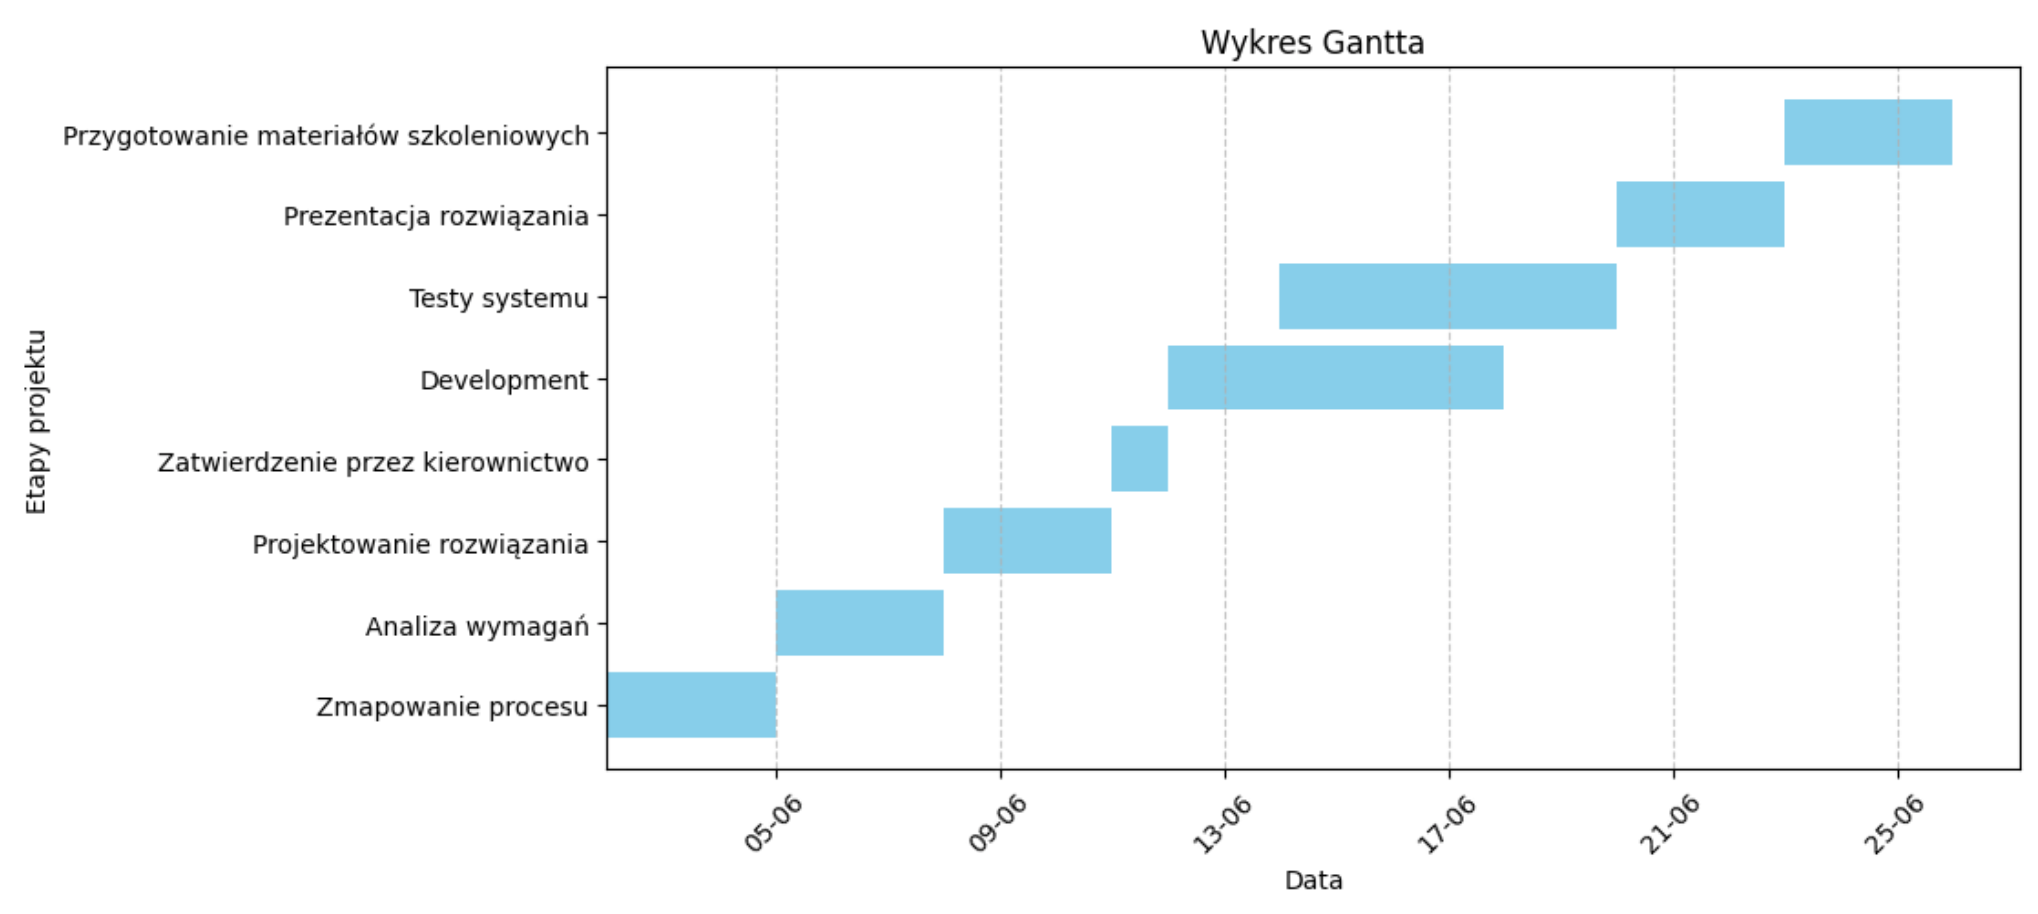
\includegraphics[width=1\linewidth]{rysunki/gantt2.png}
	\caption{Plan pracy przedstawiony na wykresie Gantta, źródło: opracowanie własne}
	\label{rys:registration}
\end{figure}

Pierwszym etapem było zmapowanie istniejącego procesu zarządzania danymi, co pozwoliło na identyfikację obszarów wymagających optymalizacji. Następnie przeprowadzono szczegółową analizę wymagań, uwzględniając potrzeby zarówno organizacyjne, jak i technologiczne. Po zatwierdzeniu specyfikacji przez kierownika projektu nastąpił etap opracowania rozwiązania i konsultacji z kierownictwem inkubatora w celu finalnej akceptacji przyjętej koncepcji.

Proces developmentu obejmował konfigurację środowiska dostępnego dla organizacji, nadanie uprawnień dla odpowiednich grup użytkowników, a także implementację przepływów pracy w \gls{powerautomate} i \gls{powerquery}. Kolejnym krokiem było przeprowadzenie testów systemu, początkowo przez programistę, a następnie przez kierownika projektu, co pozwoliło na weryfikację zgodności funkcjonalnej. Po pozytywnym zakończeniu testów rozwiązanie zostało zaprezentowane przed całym zespołem inkubatora. Ostateczna faza obejmowała opracowanie materiałów szkoleniowych w formie filmu instruktażowego oraz szczegółowego przewodnika krok po kroku, które miały zapewnić płynne wdrożenie systemu w codziennej pracy organizacji.

Harmonogram prac przewidywał realizację całego projektu w ciągu jednego miesiąca. Takie podejście pozwoliło na szybkie wdrożenie optymalizacji, minimalizując zakłócenia w bieżącej działalności inkubatora.


\chapter{Projektowanie zautomatyzowanego systemu}
W poprzednich rozdziałach zidentyfikowano problem, kontekst oraz plan projektowy – teraz nadszedł moment, by przedstawić odpowiedź: architekturę systemu, który usprawni zarządzanie danymi i automatyzację procesów. Ale dlaczego właśnie taką? Co sprawiło, że przyjęto konkretne założenia, a inne odrzucono? Jak przebiegał proces decyzyjny, który doprowadził do ostatecznej formy rozwiązania?

Projektowanie architektury to nie tylko kwestia technicznych decyzji – to poszukiwanie balansu między funkcjonalnością, wydajnością i bezpieczeństwem, a także uwzględnienie ograniczeń i przyszłych potrzeb użytkowników. W tym rozdziale przedstawione zostaną kolejne etapy tego procesu, począwszy od analizy wymagań, poprzez wybór kluczowych komponentów, aż po podejmowanie decyzji architektonicznych, które zdeterminowały finalną formę systemu.

\section{Definicja wymagań funkcjonalnych i niefunkcjonalnych}
Po zrozumieniu problemu i podstawowych założeń, określono wymagania funkcjonalne i niefunkcjonalne dla systemu automatyzacji danych Sciencepreneurs Club. System miał przede wszystkim umożliwić automatyzację procesu rejestracji uczestników i usprawnić zarządzanie danymi w \gls{cinn}.

Funkcjonalnie system został zaprojektowany, aby realizować rejestrację użytkowników poprzez formularz Microsoft Forms, gdzie dane są automatycznie przetwarzane i zapisywane w centralnej bazie \gls{excel}. Świadomie zrezygnowano z ręcznego dopisywania uczestników, redukując tym samym ryzyko pomyłek i utraty danych. System zapewnia zarządzanie danymi w dynamicznej strukturze, umożliwiającej analizę i raportowanie, a także analizę frekwencji poprzez przetwarzanie danych rejestracyjnych przez \gls{powerquery}.

W zakresie wymagań niefunkcjonalnych priorytetem stały się efektywność operacyjna i bezpieczeństwo danych.

Proces rejestracji działa autonomicznie w tle, eliminując konieczność bieżącej ingerencji administratora. System automatycznie przetwarza dane od momentu wypełnienia formularza do wprowadzenia ich do bazy. Choć przygotowanie nowej edycji wymaga rozszerzonej konfiguracji przez administratora, rezultatem jest w pełni zautomatyzowany proces niewymagający bieżących interwencji, co zapewnia wysoką efektywność operacyjną w długiej perspektywie.

System uwzględnia aspekty ochrony danych osobowych - wszystkie informacje uczestników są przechowywane w zasobach \gls{inin} zgodnie z polityką bezpieczeństwa wchodzących w \gls{microsoft365}. Rozwiązanie korzysta z wielowarstwowej architektury zabezpieczeń, która obejmuje zarówno mechanizmy na poziomie platformy, jak i specyficzne zabezpieczenia implementowane na poziomie poszczególnych komponentów. 

Również niezawodność jest jednym z kluczowych kryteriów wymagań niefunkcjonalnych. System bazuje na sprawdzonej infrastrukturze \gls{microsoft365}, co gwarantuje wysoką dostępność zgodnie z umową \gls{sla} na poziomie 99,9\%. W przypadku potrzeby przywrócenia danych, historia wersji plików przechowywana w \gls{sharepoint} umożliwia bezpieczne odtworzenie wcześniejszych zapisów. 

Dzięki przyjętej architekturze, system jest elastyczny i nie wymaga wyłączania podczas aktualizacji – wszelkie zmiany wprowadzane są poprzez duplikację i edycję istniejących elementów, co eliminuje ryzyko przerwy w działaniu w trakcie trwającej rejestracji. 

\section{Decyzje Technologiczne}
Projektowanie systemu zarządzania danymi dla \gls{cinn} było nie tylko kwestią doboru odpowiednich narzędzi, lecz także strategiczną decyzją, która miała kluczowe konsekwencje dla jego wdrożenia i późniejszego utrzymania. Wybór technologii stanowił element długotrwałych rozważań, w których uwzględniano zarówno potrzeby organizacyjne, jak i istniejące ograniczenia infrastrukturalne.

Już na wczesnym etapie rozważań pojawiła się idea stworzenia systemu opartego na relacyjnej bazie danych \gls{sql}. Logika tego rozwiązania była oczywista – umożliwiałoby ono lepszą integralność danych, automatyzację procesów, a także zapewniało wyższy poziom bezpieczeństwa i łatwość zarządzania kopiami zapasowymi. Dodatkowo, w perspektywie długoterminowej, migracja na SQL mogłaby uprościć dalszą automatyzację i integrację z innymi systemami uczelnianymi. Jednak decyzja ta nie należała wyłącznie do zespołu projektowego. Kluczowe było stanowisko kierownictwa \gls{inin}, które – analizując koszty i realia organizacyjne – uznało, że wdrożenie nowego systemu bazodanowego byłoby zbyt dużym wyzwaniem w kontekście bieżących zmian technologicznych.

\gls{inin} znajdował się w fazie stopniowej migracji do chmury, a większość danych wciąż była przechowywana w klasycznej strukturze folderów on-prem. Implementacja \gls{sql} oznaczałaby konieczność restrukturyzacji istniejących procesów, co wiązałoby się z dodatkowymi kosztami operacyjnymi oraz koniecznością zapewnienia specjalistycznej obsługi. W tym kontekście uzasadnionym wyborem stało się pozostanie przy rozwiązaniach już stosowanych w organizacji – zwłaszcza tych dostępnych w ramach licencji \gls{microsoft365}.

Alternatywne podejście, które ostatecznie przyjęto, zakładało wykorzystanie \gls{excel} jako głównej bazy danych, przy jednoczesnym zastosowaniu \gls{powerautomate} i \gls{powerquery} do automatyzacji procesów. Dzięki temu można było uniknąć konieczności kosztownej migracji, a jednocześnie zapewnić sprawną organizację danych i ich analizę w ramach istniejącej infrastruktury. Co więcej, to rozwiązanie pozwalało na szybkie wdrożenie systemu bez potrzeby angażowania dodatkowych zasobów \gls{it} oraz umożliwiało łatwe zarządzanie przez osoby nieposiadające specjalistycznej wiedzy technicznej.

Decyzja ta nie była wolna od kompromisów. \gls{excel}, mimo swojej elastyczności, nie jest narzędziem stworzonym do obsługi dużych zbiorów danych, co rodziło pytania o skalowalność i wydajność systemu w przypadku dalszego rozwoju projektu. Niemniej jednak, w warunkach \gls{inin}, gdzie priorytetem było szybkie wdrożenie i utrzymanie zgodności z obecnym środowiskiem \gls{it}, wybór ten okazał się najbardziej praktyczny. W przyszłości możliwe będzie ponowne rozważenie implementacji bazy danych \gls{sql}.
Tym samym, proces decyzyjny nie polegał jedynie na wyborze technologii, lecz na znalezieniu rozwiązania najbardziej optymalnego w kontekście realiów organizacyjnych. Elastyczność w podejściu do wyboru technologii jest kluczowym aspektem projektowania rozwiązań dla instytucji przechodzących transformację cyfrową.

\section{Architektura zabezpieczeń}

Architektura zabezpieczeń systemu Sciencepreneurs Club implementuje wielowarstwowe podejście do ochrony danych, wykorzystując zarówno mechanizmy platformy \gls{microsoft365}, jak i specyficzne zabezpieczenia na poziomie poszczególnych komponentów. Łącząc uwierzytelnianie uczelniane, autoryzację opartą o role, szyfrowanie danych, historię wersji i automatyczne kopie zapasowe, system zapewnia solidną ochronę przed typowymi zagrożeniami.

\begin{figure}[!hb]
	\centering 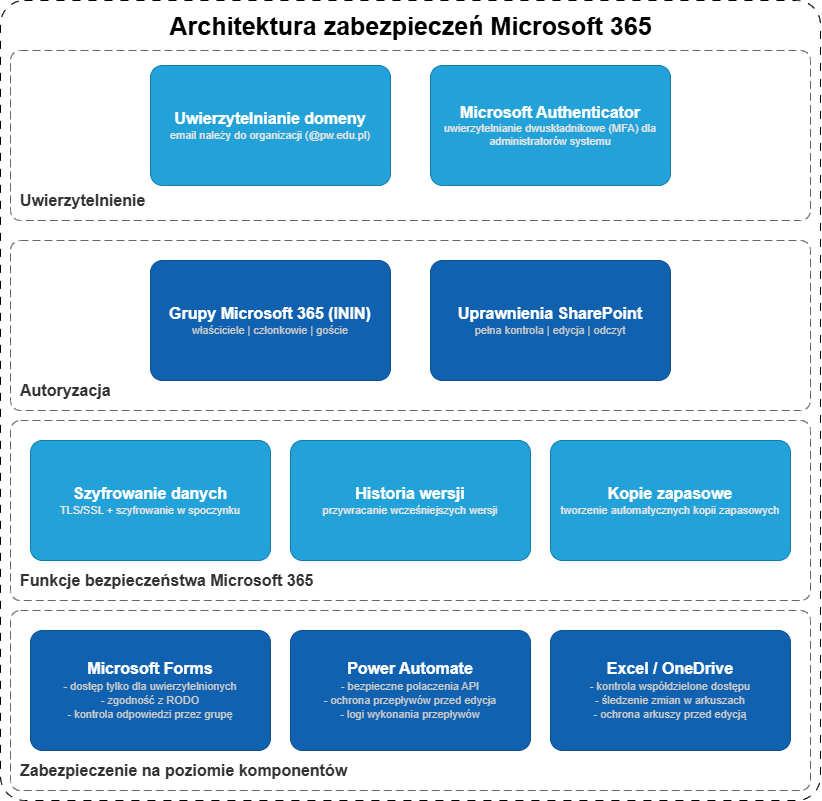
\includegraphics[width=0.85\linewidth]{rysunki/ArchitekturaZabezpieczen.png}
	\caption{Architektura zabezpieczeń systemu automatyzacji baz danych dla Sciencepreneurs Club w, źródło: opracowanie własne}
\end{figure}

Uwierzytelnianie stanowi pierwszą linię obrony w architekturze bezpieczeństwa systemu, zapewniając weryfikację tożsamości wszystkich użytkowników wchodzących w interakcję z aplikacją. Fundamentem bezpieczeństwa systemu jest \gls{entraid}. Ten centralny system zarządzania tożsamościami pozwala użytkownikom logować się do zasobów przy użyciu kont uczelnianych z domeną @pw.edu.pl, niezależnie od urządzenia, z którego korzystają. \gls{entraid} obejmuje również integrację z aplikacją Microsoft Authenticator, która korzysta z funkcjonalności \gls{mfa}. Jest to szczególnie istotne dla administratorów systemu, zapewniając dodatkową ochronę przed nieautoryzowanym dostępem nawet w przypadku kompromitacji hasła.

\begin{figure}[!hb]
	\centering 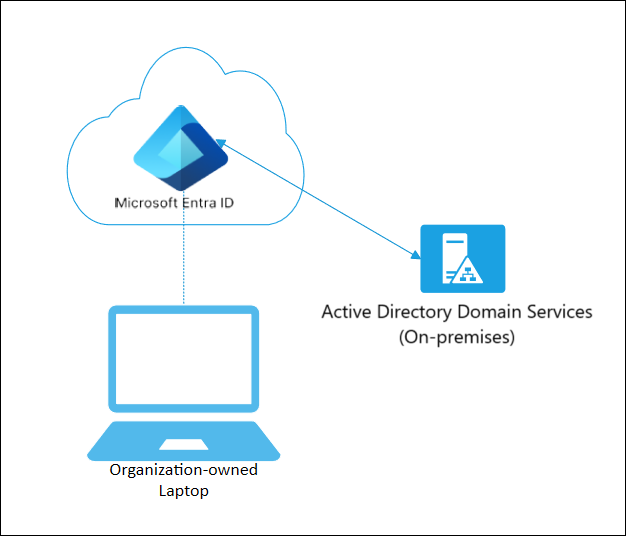
\includegraphics[width=0.7\linewidth]{rysunki/entraid.png}
	\caption{Autentykacja dostępu za pomocą \gls{entraid} , źródło: \cite{microsoft_entra_devices_2025}}
\end{figure}

Kluczową zaletą architektury opartej na \gls{entraid} jest uniezależnienie dostępu od konkretnego sprzętu. Członkowie zespołu mogą korzystać z dowolnego komputera lub urządzenia mobilnego, mając pewność, że po uwierzytelnieniu uzyskają dostęp do wszystkich zasobów grupy przechowywanych w chmurze. W przypadku awarii sprzętu, zgubienia urządzenia lub wymiany komputera, nie ma potrzeby rekonfiguracji dostępów – wszystkie uprawnienia są powiązane z kontem użytkownika w \gls{entraid}, a nie z fizycznym urządzeniem. Eliminuje to przestoje związane z problemami technicznymi i zapewnia ciągłość pracy.
\gls{entraid}  integruje się z systemami zarządzania cyklem życia kont na uczelni, co gwarantuje automatyczną dezaktywację dostępu dla osób, które przestały być związane z \gls{pw}. \cite{microsoft_entra_devices_2025} 

Po pomyślnym uwierzytelnieniu, warstwa autoryzacji definiuje precyzyjny zakres dostępu użytkownika do konkretnych zasobów i funkcji. System implementuje model kontroli dostępu oparty o role poprzez grupy \gls{microsoft365}. \cite{Microsoft365Groups2025} Podstawą organizacji uprawnień jest grupa \texttt{"Inkubator\_PW"} z trzema poziomami dostępu. 
Właściciele posiadają pełen dostęp administracyjny do wszystkich komponentów systemu. Członkowie – ze standardowym dostępem operacyjnym mają wgląd do przeglądania i ograniczonej edycji. Na najniższym poziomie są goście, z dostępem tylko do odczytu wybranych zasobów. Uzupełnieniem są szczegółowe uprawnienia \gls{sharepoint} na poziomie repozytorium dokumentów (pełna kontrola, edycja, odczyt), zapewniające precyzyjną kontrolę zgodną z zasadą minimalnych uprawnień.

Platforma \gls{microsoft365} oferuje szereg wbudowanych mechanizmów bezpieczeństwa wykorzystywanych w systemie. Szyfrowanie danych obejmuje zarówno szyfrowanie transmisji (\gls{tls}/\gls{ssl}) jak i szyfrowanie danych w spoczynku. \cite{microsoft_encryption_2024} Historia wersji zapewnia automatyczne śledzenie zmian w dokumentach z możliwością przywracania wcześniejszych wersji. Dodatkowo system korzysta z automatycznych kopii zapasowych.

Każdy z trzech głównych komponentów systemu implementuje dodatkowe mechanizmy bezpieczeństwa. \gls{forms} wprowadza implementację klauzul zgodnych z \gls{rodo}. Power Automate zapewnia bezpieczne połączenia \gls{api} z uwierzytelnianiem ustandaryzowanym wewnątrz środowiska \gls{microsoft365}. \cite{microsoft_encryption_2024}. \gls{excel} i \gls{onedrive} dostarczają kontrolę współdzielonego dostępu, śledzenie zmian w arkuszach, selektywną ochronę arkuszy i zakresów komórek przed edycją oraz zdefiniowane role dostępu. \cite{microsoft_office_versions_2025} \cite{microsoft_excel_blocking_2025}

Architektura zabezpieczeń systemu Sciencepreneurs Club stanowi wielowarstwowy system ochrony, który łączy mechanizmy \gls{entraid}, kontroli dostępu bazującej na rolach, szyfrowania danych oraz specyficznych zabezpieczeń komponentowych. Takie podejście zapewnia odpowiedni poziom bezpieczeństwa przy jednoczesnym zachowaniu elastyczności i użyteczności systemu.

\section{Diagram czynności}

Proces rejestracji uczestników wydarzeń opiera się na zautomatyzowanym systemie, który minimalizuje konieczność ręcznej obsługi zgłoszeń. Każda nowa edycja wydarzenia rozpoczyna się od wykonania przez administratora zestawu powtarzalnych czynności przygotowawczych. Zadania, które nadal wymagają manualnej interwencji, zostały precyzyjnie zmapowane, co umożliwia ich przyszłą automatyzację w kolejnych etapach rozwoju systemu.

\newpage
\begin{figure}[!hb]
	\centering 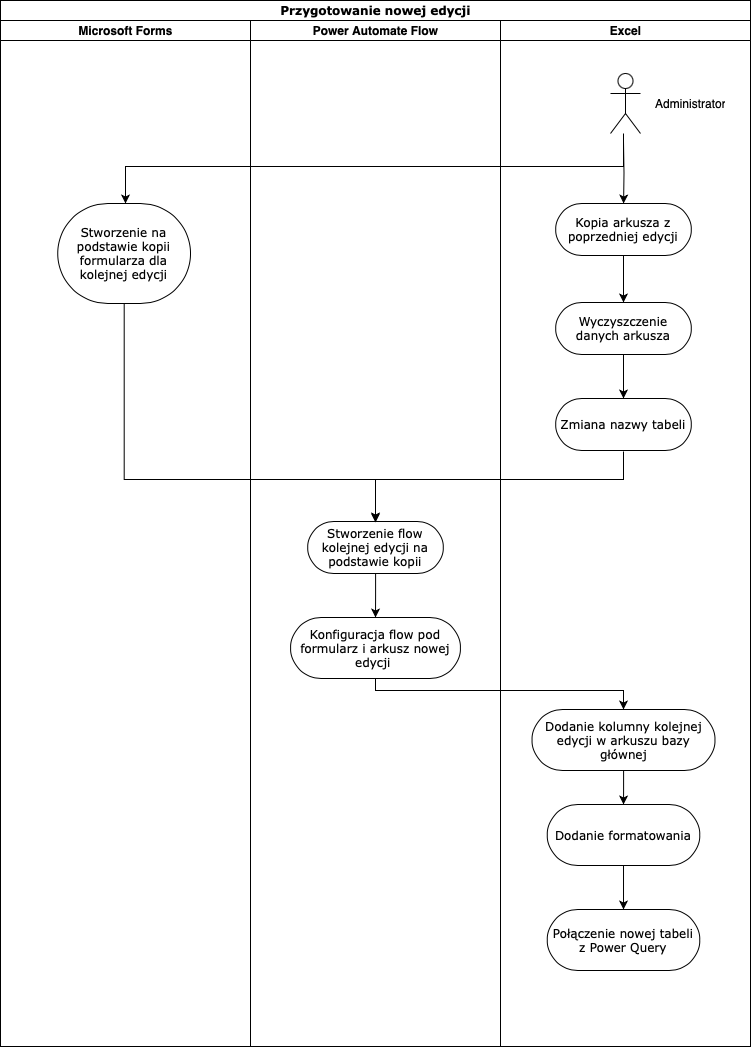
\includegraphics[width=0.85\linewidth]{rysunki/przygotowanie.png}
	\caption{Przygotowanie na kolejną edycję - administrator, źródło: opracowanie własne }
\end{figure}

Każda nowa edycja wydarzenia wymaga uprzedniego przygotowania przez administratora. Proces ten rozpoczyna się od organizacji bazy danych, co obejmuje skopiowanie arkusza z poprzedniej edycji, usunięcie wcześniejszych wpisów, nadanie nowej nazwy oraz dostosowanie istniejących formuł. Równocześnie tworzony jest nowy formularz rejestracyjny na podstawie wzorca z poprzedniego wydarzenia, z uwzględnieniem zmiany nazwy, prelegenta, tematu oraz terminu. Następnie konieczna jest aktualizacja przepływu pracy w \gls{powerautomate}, polegająca na skopiowaniu istniejącego procesu, dostosowaniu nazwy oraz podpięciu nowego formularza i tabeli w bazie danych. Ostatnim etapem konfiguracji jest uaktualnienie raportów poprzez dodanie nowej edycji do głównej bazy danych, wprowadzenie reguł formatowania dla nowej daty oraz aktualizację źródeł w \gls{powerquery}. Po wykonaniu tych kroków dalszy przebieg rejestracji odbywa się bez konieczności nadzoru ze strony administratora – wszystkie zgłoszenia są automatycznie zapisywane i przetwarzane.

\begin{figure}[!hb]
	\centering 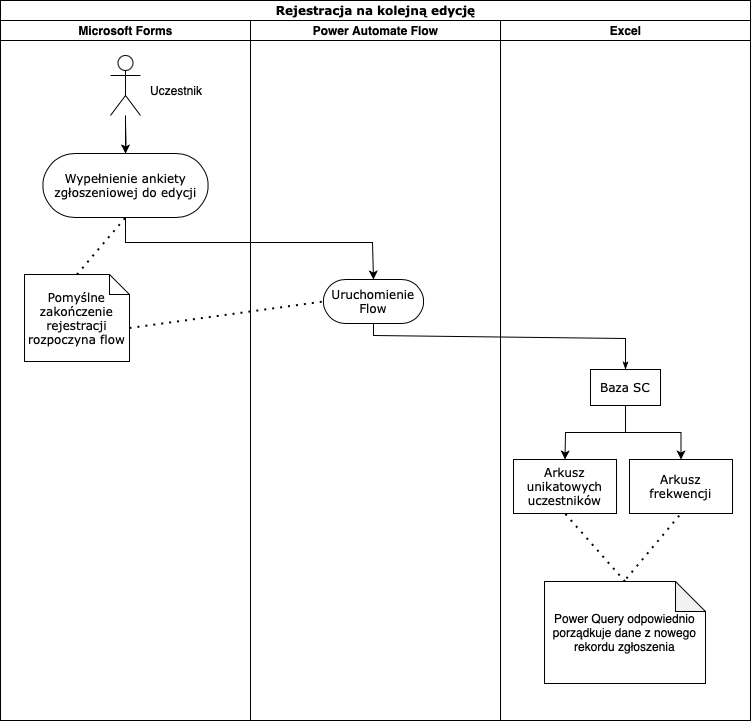
\includegraphics[width=0.85\linewidth]{rysunki/registration.png}
	\caption{Rejestracja na kolejną edycję - uczestnik, źródło: opracowanie własne}
\end{figure}

Uczestnicy otrzymują link do formularza rejestracyjnego stworzonego w Microsoft Forms, gdzie podają podstawowe informacje, takie jak imię, nazwisko, adres e-mail oraz temat wydarzenia. Po przesłaniu formularza dane są automatycznie przekazywane do centralnej bazy danych w arkuszu Excel za pośrednictwem przepływu pracy skonfigurowanego w \gls{powerautomate}. Dzięki temu administrator nie musi podejmować żadnych dodatkowych działań – zgłoszenia są zapisywane w bazie w sposób całkowicie zautomatyzowany.

\section{Architektura systemu}
Architektura systemu zarządzania uczestnikami Sciencepreneurs Club została zaprojektowana zgodnie z podejściem warstwowym, gdzie każdy komponent odpowiada za ściśle określony obszar funkcjonalny. Jednocześnie, dzięki wykorzystaniu platformy \gls{microsoft365}, zapewniono wysoki poziom integracji między poszczególnymi elementami.

\begin{figure}[!ht]
\centering
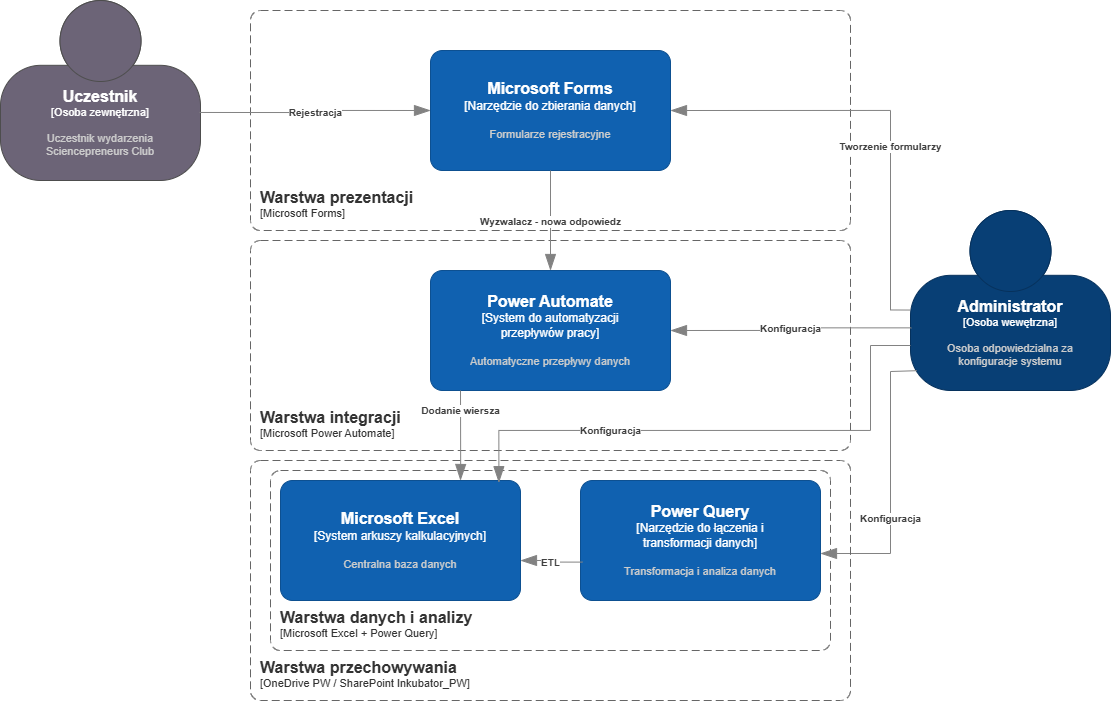
\includegraphics[width=1\linewidth]{rysunki/ArchitekturaSystemu.PNG}
\caption{Architektura systemu zarządzania uczestnikami Sciencepreneurs Club, żródło: opracowanie własne}
\label{fig}
\end{figure}

System charakteryzuje się architekturą warstwową, gdzie:

\begin{itemize}
\item \textbf{Warstwa prezentacji} – realizowana przez \gls{forms}, odpowiada za interakcję z użytkownikiem końcowym (uczestnikiem).
\item \textbf{Warstwa integracji} – implementowana przez \gls{powerautomate}, zarządza przepływem danych między poszczególnymi komponentami.
\item \textbf{Warstwa danych i analizy} – obsługiwana przez \gls{excel} z \gls{powerquery}, pełni funkcję centralnego repozytorium i narzędzia analitycznego.
\end{itemize}

Szczególną cechą systemu jest wykorzystanie chmury Azure do przechowywania komponentów, eliminując w ten sposób konieczność lokalnej instalacji oprogramowania co zapewnia dostęp do danych z dowolnej lokalizacji i znacząco zwiększa elastyczność w zarządzaniu. Jednocześnie, przechowywanie danych w ramach infrastruktury \gls{microsoft365} \gls{pw} zapewnia odpowiedni poziom bezpieczeństwa i zgodność z politykami uczelnianymi.

Warstwa prezentacji architektury, zaimplementowana przy użyciu \gls{forms}, odpowiada za komunikację z użytkownikami końcowymi i zbieranie danych wejściowych. W tej warstwie realizowane są dwa główne działania proces wypełniania formularza rejestracyjnego przez potencjalnego uczestnika wydarzenia oraz 
zestaw działań administracyjnych obejmujących tworzenie, modyfikowanie i publikowanie formularzy dla kolejnych edycji wydarzenia.

Warstwa integracji, środkowa warstwa, oparta na \gls{powerautomate}, pełni funkcję łącznika między interfejsem użytkownika a systemem przechowywania danych. Kluczową rolą tej warstwy jest automatyzacja przepływu pracy poprzez:wykrywanie nowych odpowiedzi w formularzach (wyzwalacze), transformację danych z formatu formularza do struktury bazy danych oraz zapewnienie niezawodnego zapisu danych w czasie rzeczywistym. \gls{powerautomate} eliminuje potrzebę ręcznej interwencji w procesie transferu danych, minimalizując ryzyko błędu ludzkiego i zapewniając natychmiastową dostępność nowych danych w systemie.


Najniższa warstwa systemu (danych i analizy) jest przechowywana bezpośrednio w \gls{onedrive} \gls{pw} w folderze \texttt{"Inkubator\_PW"} który jest środowiskiem hostującym dla pliku \gls{excel} \texttt{"SC BAZA.xlsx"}.

W ramach tego pliku \gls{excel} wyróżniamy dwa główne komponenty:
\begin{itemize}
\item \textbf{\gls{excel}} - struktura arkuszy przechowująca dane w uporządkowany sposób:
\begin{itemize}
\item Baza (unikatowi uczestnicy) - lista deduplikowanych uczestników
\item Baza (wszystkie rejestracje) - pełny rejestr zgłoszeń
\item Uczestnicy \#1, \#2, \#3... - dane z poszczególnych edycji
\end{itemize}
\item \textbf{\gls{powerquery}} - wbudowany w plik \gls{excel} mechanizm \gls{etl}), realizujący:
\begin{itemize}
\item Deduplikację uczestników
\item Konsolidację danych z różnych edycji
\item Transformację danych na potrzeby analityczne
\end{itemize}
\end{itemize}

Istotne jest zrozumienie, że \gls{excel} i \gls{powerquery} nie są oddzielnymi aplikacjami wysyłającymi dane do \gls{onedrive}, ale funkcjonują jako jeden plik przechowywany w chmurze, gdzie wszystkie operacje przetwarzania danych odbywają się bezpośrednio w środowisku \gls{onedrive} \gls{pw}.


Trójwarstwowe podejście do modelowania architektury systemu nie tylko odzwierciedla rzeczywistą implementację, ale również podkreśla zalety wykorzystania zintegrowanego ekosystemu chmurowego. System charakteryzuje się prostotą implementacyjną przy jednoczesnym zapewnieniu wymaganej funkcjonalności, co czyni go optymalnym rozwiązaniem dla struktury organizacyjnej i skali projektu Sciencepreneurs Club.





\chapter{Komponenty projektu inżynierskiego}
System zarządzania uczestnikami Sciencepreneurs Club stanowi przykład nowoczesnego podejścia do digitalizacji procesów organizacyjnych w środowisku akademickim. W świecie, gdzie efektywne zarządzanie danymi staje się kluczowym czynnikiem sukcesu inicjatyw edukacyjnych, implementacja zintegrowanych rozwiązań chmurowych nabiera szczególnego znaczenia. Rozdział ten prezentuje kompleksową analizę architektury systemu, który powstał jako odpowiedź na wyzwania związane z koordynacją cyklicznych wydarzeń klubu studenckiego.

Ten zautomatyzowany system opiera się na trzech kluczowych komponentach funkcjonalnych: \gls{forms}, \gls{powerautomate} oraz \gls{excel} wzbogacony o funkcjonalność \gls{powerquery}. Każdy z tych elementów, choć może funkcjonować niezależnie, w ramach opisywanego rozwiązania tworzy spójny łańcuch przetwarzania danych – od momentu rejestracji uczestnika, przez automatyzację przepływu informacji, aż po podstawową analizę danych frekwencji.

\section{Warstwa prezentacji - Microsoft Forms}

\gls{forms} to intuicyjna platforma do tworzenia formularzy i ankiet, które mogą być bezpośrednio powiązane z innymi narzędziami \gls{microsoft365}. W kontekście Sciencepreneurs Club, \gls{forms} pełni rolę frontendu całego systemu – jest pierwszym punktem kontaktu potencjalnego uczestnika. To właśnie za pomocą tego narzędzia realizowany jest proces rejestracji na poszczególne wydarzenia klubowe, stanowiąc cyfrową bramę wejściową do ekosystemu danych projektu.

Dostęp do formularzy jest ściśle kontrolowany poprzez hierarchiczny system uprawnień \cite{Microsoft365Groups2025}:

\begin{table}[ht]
\centering
\caption[Hierarchiczny system uprawnień do formularzy, źródło: dokumentacja Microsoft 365, omówienie grup dostępu dla administratorów \cite{Microsoft365Groups2025}]{Hierarchiczny system uprawnień do formularzy}
\renewcommand{\arraystretch}{1.3} % Zwiększenie odstępów między wierszami
\begin{tabular}{| >{\raggedright\arraybackslash}p{0.25\textwidth} | >{\raggedright\arraybackslash}p{0.65\textwidth} |}
\hline
\textbf{Poziom uprawnień} & \textbf{Zakres dostępu i możliwości} \\
\hline
Właściciele grupy (Group Owners) & Pełne uprawnienia administracyjne: tworzenie nowych formularzy, modyfikacja istniejących, zarządzanie dostępem innych użytkowników \\
\hline
Członkowie grupy (Group Members) & Przeglądanie i edytowanie formularzy z ograniczeniami dotyczącymi konfiguracji zaawansowanych ustawień bezpieczeństwa \\
\hline
Użytkownicy zewnętrzni & Ograniczony dostęp: wypełnianie formularzy bez możliwości dostępu do wyników lub ustawień (zależnie od konfiguracji formularza) \\
\hline
\end{tabular}
\vspace{0.5em}
\par\raggedright\footnotesize{Źródło: dokumentacja Microsoft 365, omówienie grup dostępu dla administratorów \cite{Microsoft365Groups2025}}
\end{table}

\gls{forms} oferuje wielopoziomowy system kontroli dostępu, który jest kluczowy dla zachowania integralności danych w środowisku akademickim. W implementacji dla Sciencepreneurs Club zastosowano model bezpieczeństwa oparty na grupach \gls{microsoft365}, gdzie wszystkie formularze są przechowywane w dedykowanej grupie \gls{inin}.

\gls{forms} implementuje kompleksowe mechanizmy ochrony danych, które stanowią istotny element strategii bezpieczeństwa informacji. Cała infrastruktura została zaprojektowana zgodnie z najwyższymi standardami branży \gls{it} zachowując zgodność z wymogami prawnymi oraz wielopoziomowe zabezpieczenia danych. 

\gls{forms} spełnia wymagania \gls{rodo} od momentu jego wejścia w życie w maju 2018 roku. Dodatkowo, platforma jest zgodna z ustawą \gls{hipaa} oraz umową \gls{baa}, co czyni ją odpowiednią do zastosowań w sektorach wrażliwych, takich jak ochrona zdrowia czy edukacja (zgodność z \gls{ferpa}). \cite{microsoft_forms_privacy_2024} Microsoft regularnie aktualizuje swoje rozwiązania w odpowiedzi na zmieniające się zagrożenia cybernetyczne oraz wymogi prawne, zapewniając stałą ochronę danych użytkowników przy jednoczesnym zachowaniu funkcjonalności i wygody korzystania z platformy.

Dane przechowywane na serwerach Microsoft są chronione na dwóch kluczowych poziomach \cite{microsoft_encryption_2024}:
\begin{itemize}
    \item \textbf{W czasie spoczynku} – wszystkie informacje zapisane na dyskach serwerów Microsoft podlegają szyfrowaniu. Oznacza to, że nawet w przypadku nieuprawnionego dostępu fizycznego do nośników, dane pozostają nieczytelne bez odpowiednich kluczy deszyfrujących.
    \item \textbf{Podczas tranzytu} – transmisja danych między użytkownikiem a serwerami (np. podczas wypełniania i przesyłania formularzy) jest zabezpieczona protokołem \gls{https}. Ta technologia efektywnie uniemożliwia przechwycenie informacji przez podmioty nieuprawnione podczas ich przesyłania przez sieć.
\end{itemize}

Istotną zaletą \gls{forms} w kontekście cyklicznych wydarzeń klubowych jest możliwość replikacji istniejących formularzy. Formularze z poprzednich edycji są zachowane nie tylko w celu archiwalnym, ale także jako szablon pod kolejne wydarzenia. Administrator w celu przygotowania nowej edycji kopiuje formularz z poprzedniej i uzupełnia informacje organizacyjne o najnowsze, takie jak numer edycji, prelegent, data, miejsce i temat spotkania. 

Po przygotowaniu formularza na kolejną edycję zostaje on opublikowany przez administratora. Uczestnicy za pomocą linku do formularza  wypełniają w nim kluczowe informacje zgłoszeniowe, takie jak imię i nazwisko, adres e-mail, zgoda na przetwarzanie danych oraz datę rejestracji.

Po pomyślnym wypełnieniu formularza, dane uczestnika są automatycznie przekazywane do dalszego przetwarzania poprzez integrację z \gls{powerautomate}, stanowiąc pierwszy etap zautomatyzowanego cyklu zarządzania danymi w ekosystemie Sciencepreneurs Club.

\section{Warstwa integracji - Power Automate}

\gls{powerautomate} (wcześniej Microsoft Flow) to narzędzie do tworzenia zautomatyzowanych przepływów pracy. W Sciencepreneurs Club pełni funkcję pośrednika między \gls{forms} a \gls{excel}. To właśnie w nim zakodowane jest automatyczne przekazywanie danych uczestników po wypełnieniu zgłoszenia do bazy danych „SC BAZA.xlsx”. 

\begin{figure}[!hb]
	\centering 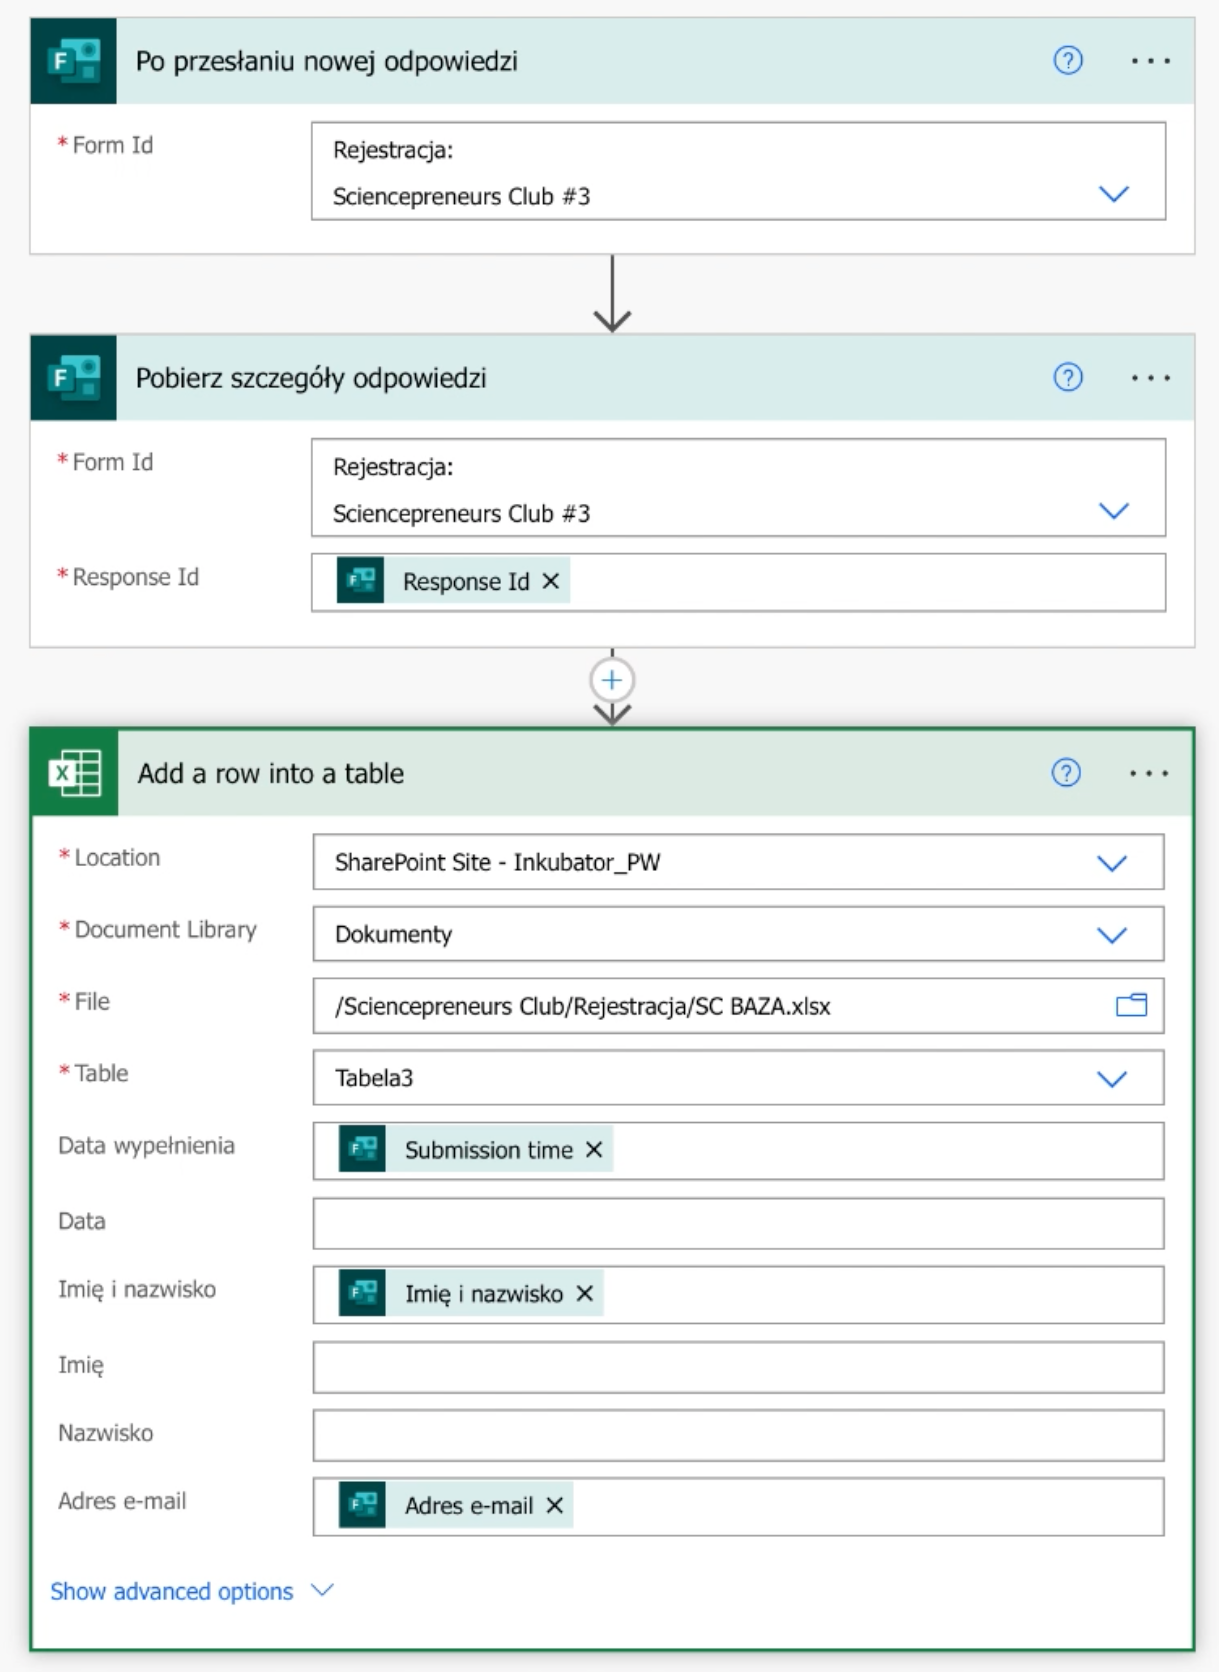
\includegraphics[width=0.7\linewidth]{rysunki/flow3.png}
	\caption{Power Automate Flow dla trzeciej edycji Sciencepreneurs Club, źródło: opracowanie własne }
\end{figure}

Dzieje się to poprzez poszczególne etapy przepływu pracy. 
Pierwszym z nich jest wyzwalacz. Każda nowa odpowiedź w Forms rozpoczyna działanie "Flow", gdy uczestnik wypełni formularz rejestracyjny. Aktywacja przepływu następuje automatycznie w momencie złożenia nowego zgłoszenia w formularzu \gls{forms}. \cite{microsoft_power_automate_2025} Wyzwalacz \gls{powerautomate} funkcjonuje na zasadzie nasłuchiwania określonych zdarzeń w połączonych aplikacjach. W przypadku Sciencepreneurs Club, wyzwalacz jest skonfigurowany do monitorowania konkretnego formularza \gls{forms}, zidentyfikowanego przez unikalny identyfikator widoczny w polu "Form Id". Jednak nie ma potrzeby kopiowania ID formularza, narzędzie zostało przygotowane w ten sposób, że wystarczy wybrać odpowiednią nazwę z listy, jak na rysunku 7.1. Poprawne powiązanie Flow z formularzem jest absolutnie kluczowe dla funkcjonowania całego systemu - każda zmiana formularza wymaga aktualizacji tego identyfikatora, co jest realizowane podczas przygotowywania nowej edycji wydarzenia.

\begin{figure}[!hb]
	\centering 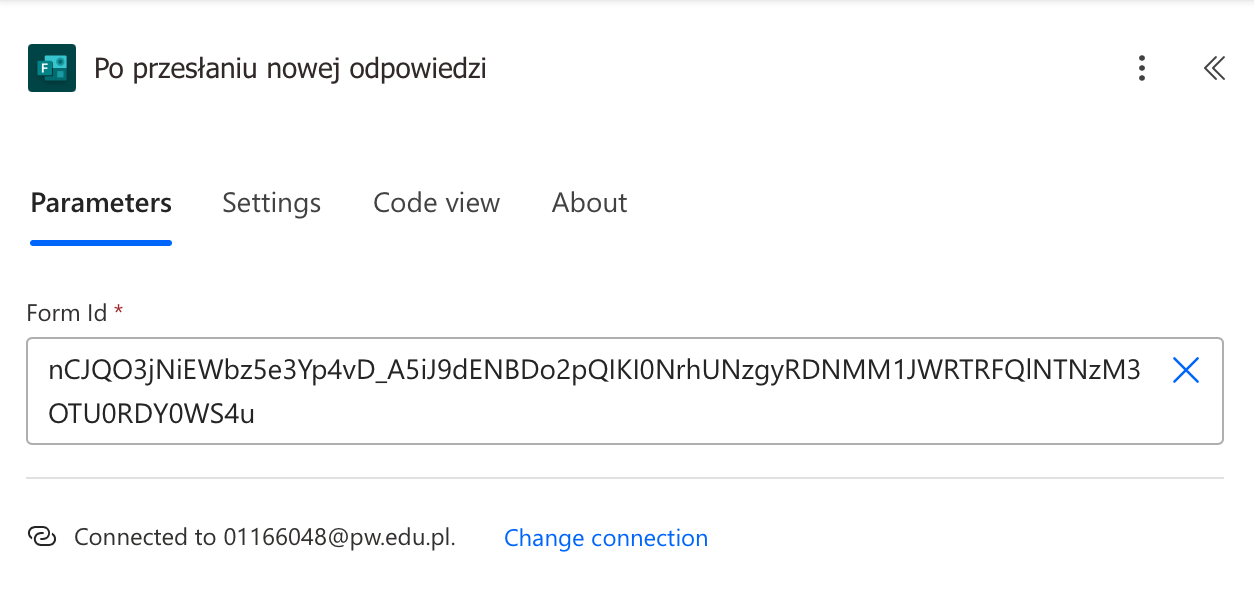
\includegraphics[width=0.7\linewidth]{rysunki/KonfiguracjaPowerAutomate.png}
	\caption{Konfiguracja wyzwalacza Power Automate Flow, źródło: opracowanie własne z użyciem narzędzia \gls{powerautomate}}
\end{figure}

Na rysunku 7.2. widać, że system jest skonfigurowany w kontekście konta uczelnianego \gls{pw} (01166048@pw.edu.pl). Jest to fundamentalny element architektury systemu, gdyż umożliwia za pomocą grup dostępu bezpośrednie połączenie do grupy Inkubator\_PW należącej do \gls{inin}. To połączenie gwarantuje dostęp do zasobów przechowywanych w \gls{onedrive} \gls{pw} oraz zachowanie ciągłości dostępu dla kolejnych administratorów systemu w ramach uczelni.

Istotnym aspektem architektury \gls{powerautomate}, który warto podkreślić, jest sposób, w jaki graficzny interfejs użytkownika współpracuje z kodem JSON stanowiącym podstawę funkcjonowania przepływów. W kontekście systemu Sciencepreneurs Club, administrator konfigurujący przepływ nie musi bezpośrednio pisać kodu. Proces konfiguracji wyzwalacza dla formularza \gls{forms} przebiega następująco:

\begin{itemize}
    \item Administrator wybiera typ wyzwalacza "Po przesłaniu nowej odpowiedzi" z galerii dostępnych wyzwalaczy Microsoft Forms.
    \item Następnie, z rozwijanej listy dostępnych formularzy, wskazuje konkretny formularz rejestracyjny dla danej edycji Sciencepreneurs Club.
    \item Power Automate automatycznie pobiera unikalny identyfikator formularza i generuje odpowiedni kod JSON w tle.
\end{itemize}

To, co widzimy w prezentowanym kodzie JSON, jest faktycznie efektem tych działań w interfejsie, a nie kodem napisanym ręcznie przez administratora. Platforma \gls{powerautomate} przetwarza wybory dokonane w interfejsie graficznym na strukturalną definicję przepływu w formacie JSON, która następnie jest interpretowana przez \gls{flowengine} pracy platformy.\cite{microsoft_power_automate_2025} W przypadku Sciencepreneurs Club, przepływ to cała sekwencja automatyzacji od momentu wypełnienia formularza przez uczestnika, przez zapisanie jego danych w \gls{excel}.

\begin{lstlisting}[language=JSON, caption=Konfiguracja wyzwalacza Power Automate w języku JSON źródło: kod wygenerowany na podstwie konfiguracji poprzez narzędzie Power Automate]
{
  "type": "OpenApiConnectionWebhook",
  "inputs": {
    "parameters": {
      "form_id": "nCJQO3jNiEWbz5e3Yp4vD_A5iJ9dENBDo2pQIKI0NrhUNzgyRDNMM1JWRTR
      FQlNTNzM3OTU0RDY0WS4u"
    },
    "host": {
      "apiId": "/providers/Microsoft.PowerApps/apis/shared_microsoftforms",
      "connection": "shared_microsoftforms",
      "operationId": "CreateFormWebhook"
    }
  },
  "splitOn": "@triggerOutputs()?['body/value']",
  "metadata": {
    "operationMetadataId": "c82c4e1e-d1d3-4721-a97a-27e2155adc56"
  }
}
\end{lstlisting}

Przedstawiony fragment kodu JSON  7.1. definiuje szczegółową konfigurację wyzwalacza. Choć ten kod nie jest pisany ręcznie przez administratora, zrozumienie jego struktury pozwala lepiej pojąć, jak działa automatyzacja w systemie.

Fragment kodu rozpoczyna się określeniem typu wyzwalacza jako \texttt{"OpenApiConnectionWebhook"}. Oznacza to, że nasz wyzwalacz wykorzystuje standardowy sposób komunikacji między usługami \gls{microsoft365}, działając jak cyfrowy czujnik nasłuchujący określonych wydarzeń.

W sekcji \texttt{"inputs"} znajdują się wszystkie informacje wejściowe potrzebne do prawidłowego działania wyzwalacza. Najważniejszym elementem jest parametr \texttt{"form\_id"}, który zawiera długi ciąg znaków jednoznacznie identyfikujący formularz \gls{forms}, który ma być monitorowany. To właśnie ten identyfikator wiąże nasz przepływ z konkretnym formularzem rejestracyjnym wydarzenia.

Dalej w kodzie znajduje się sekcja \texttt{"host"}, która określa, z jakim systemem nasz wyzwalacz będzie się komunikował. Parametr \texttt{"apiId"} wskazuje, że będziemy korzystać z \gls{api} \gls{forms}, a \texttt{"connection"} określa typ połączenia jako standardowe połączenie do \gls{forms}. Parametr \texttt{"operationId"} precyzuje, że konkretna operacja to \texttt{"CreateFormWebhook"}, czyli utworzenie mechanizmu nasłuchującego nowych odpowiedzi w formularzu.

Kolejny element, \texttt{"splitOn"} definiuje sposób, w jaki dane z formularza będą przetwarzane przez przepływ. Ta techniczna instrukcja informuje silnik przepływów, jak ma rozdzielać otrzymane odpowiedzi na poszczególne elementy danych, które będą wykorzystywane w dalszych krokach przepływu.

Na końcu znajduje się sekcja \texttt{"metadata"} zawierająca unikalny identyfikator operacji. Jest to wewnętrzny znacznik używany przez \gls{powerautomate} do śledzenia i zarządzania przepływem podczas jego wykonywania.

Wszystkie te elementy razem tworzą kompletną definicję wyzwalacza. Gdy tylko pojawi się nowa odpowiedź, wyzwalacz aktywuje się i uruchamia pozostałe kroki przepływu.

Kolejnym krokiem jest pobranie danych, \gls{powerautomate} pobiera szczegóły odpowiedzi wprowadzone przez uczestnika, wraz z metadanymi formularza i przekazuje je do \gls{excel}. Ponownie jak w pierwszym kroku wyzawalacza, należy skonfigurować do monitorowania konkretnego formularza Microsoft Forms. W tym przypadku jest to ten sam formularz (to samo ID). 

\begin{lstlisting}[language=JSON, caption=Konfiguracja pobrania szczegółów odpowiedzi z formularza w Power Automate w języku JSON źródło: kod wygenerowany na podstwie konfiguracji poprzez narzędzie Power Automate]
{
  "type": "OpenApiConnection",
  "inputs": {
    "parameters": {
      "form_id": "nCJQO3jNiEWbz5e3Yp4vD_A5iJ9dENBDo2pQIKI0NrhUNzgyRDNMM1JWRTR
      FQlNTNzM3OTU0RDY0WS4u",
      "response_id": "@triggerOutputs()?['body/resourceData/responseId']"
    },
    "host": {
      "apiId": "/providers/Microsoft.PowerApps/apis/shared_microsoftforms",
      "connection": "shared_microsoftforms",
      "operationId": "GetFormResponseById"
    }
  },
  "runAfter": {},
  "metadata": {
    "operationMetadataId": "f2fea26e-bc97-4c91-8a2b-9dc2c7fb6e4f"
  }
}
\end{lstlisting}

Podczas gdy pierwszy kod 7.1.(wyzwalacz) informował system, aby nasłuchiwał nowych odpowiedzi w formularzu, ten kod 7.2. określa, co należy zrobić, gdy taka odpowiedź się pojawi.

Typ tego kroku to \texttt{"OpenApiConnection"}, co oznacza standardowe połączenie z usługą \gls{microsoft365}. W przeciwieństwie do poprzedniego kroku, który był typu \texttt{"OpenApiConnectionWebhook"}, ten krok nie nasłuchuje zdarzeń, ale aktywnie pobiera dane.

W sekcji \texttt{"inputs"} znajdują się parametry potrzebne do pobrania szczegółowych informacji o odpowiedzi na formularz. Widzimy tu dwa ważne elementy. Pierwszy \texttt{"form\_id"} - ten sam identyfikator formularza co w poprzednim kroku, który wskazuje, z którego formularza mamy pobrać dane. Oraz \texttt{"response\_id"} - tutaj pojawia się: \texttt{"@triggerOutputs()}\texttt{['body/resourceData} \texttt{/responseId']}. Ta dynamiczna wartość pobiera identyfikator konkretnej odpowiedzi z danych wyzwalacza. Innymi słowy, system pobiera identyfikator nowo złożonego zgłoszenia, aby następnie pobrać jego szczegóły.

W sekcji \texttt{"host"} widzimy podobne informacje jak wcześniej - używamy \gls{api} \gls{forms}, ale tym razem operacja to \texttt{"GetFormResponseById"}. Nazwa ta jasno wskazuje cel: pobranie szczegółów odpowiedzi na podstawie jej identyfikatora.

Element \verb|"runAfter": {}| informuje system, że ten krok powinien zostać wykonany bezpośrednio po uruchomieniu wyzwalacza, bez żadnych dodatkowych warunków czy opóźnień.

Na koniec mamy sekcję \texttt{"metadata"} z unikalnym identyfikatorem operacji, który służy do wewnętrznego zarządzania tym krokiem w \gls{powerautomate}. Pobiera wszystkie szczegółowe informacje z formularza, gdy ktoś go wypełni. Te dane będą następnie dostępne dla kolejnych kroków przepływu.

Finalnym etapem naszego zautomatyzowanego przepływu jest zapisanie danych uczestnika w arkuszu \gls{excel} w dopasowanej kolumnie, który służy jako centralna baza danych Sciencepreneurs Club. W ten sposób każda wypełniona w \gls{forms} ankieta jest automatycznie eksportowana do pliku \gls{excel}, gdzie stanowi punkt wyjścia do dalszego przetwarzania danych. Ten krok zamyka pętlę procesu, zapewniając, że informacje wprowadzone przez uczestnika w formularzu \gls{forms} zostaną trwale przechowane i będą dostępne do dalszej analizy.

\begin{figure}[!hb]
	\centering 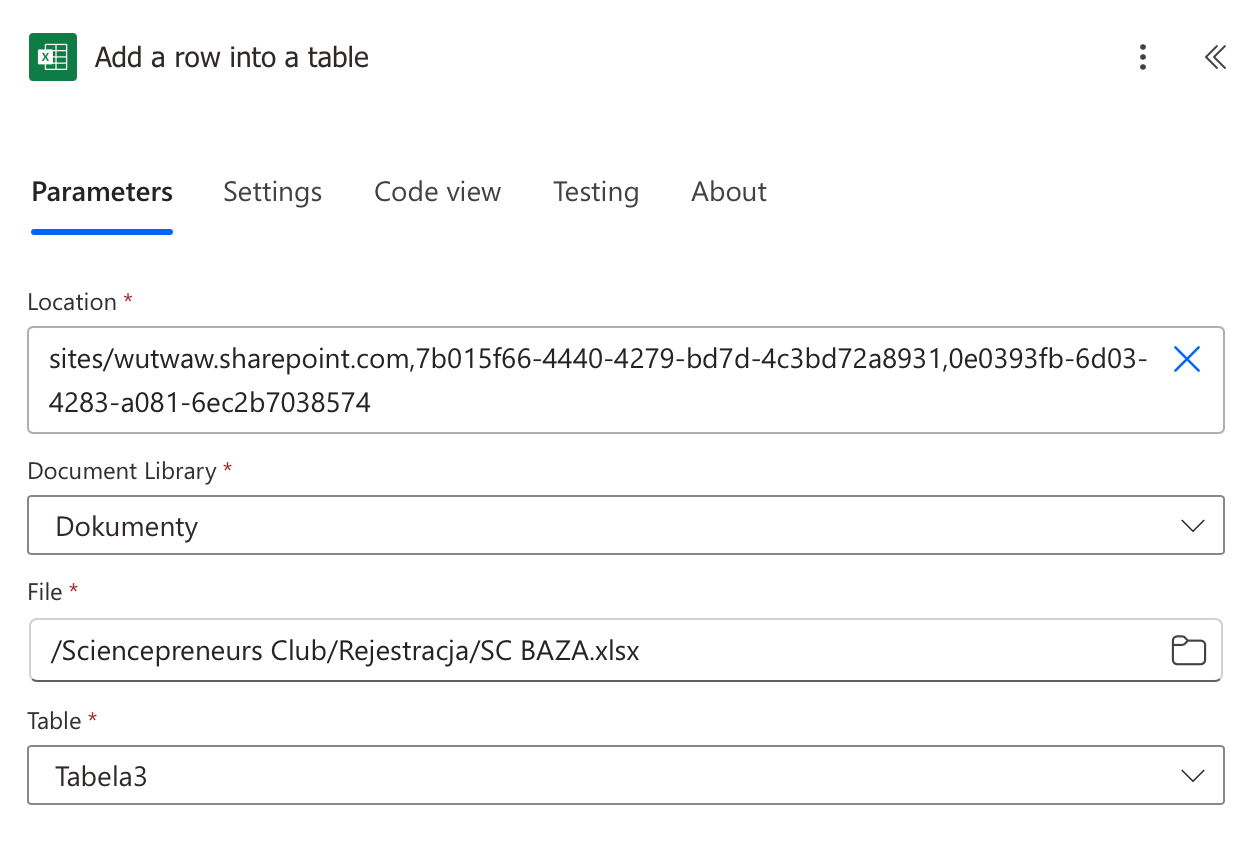
\includegraphics[width=0.7\linewidth]{rysunki/DodanieWiersza.png}
	\caption{Podstwowe parametry konfiguracji ładowania danych do nowego wiersza Microsoft Excel z użyciem Power Automate Flow, źródło: opracowanie własne z użyciem narzędzia \gls{powerautomate}}
\end{figure}

Administrator musi zdefiniować kluczowe parametry. Te wizualne wybory są następnie przekształcane przez system w precyzyjne identyfikatory w kodzie konfiguracyjnym, zapewniając jednoznaczne wskazanie miejsca docelowego dla danych uczestników. Parametry te definiują ścieżkę, którą podążą dane z formularza, aby finalnie trafić do odpowiedniego arkusza w pliku \gls{excel} przechowywanym w środowisku chmurowym \gls{microsoft365}.

W tym samym kroku administrator definiuje, które pola z formularza (identyfikowane przez unikalne identyfikatory odpowiedzi) mają zostać zapisane w jakich kolumnach tabeli \gls{excel}. Interfejs \gls{powerautomate} umożliwia wybór dynamicznych wartości z wcześniejszego kroku \texttt{"Pobierz\_szczegóły\_odpowiedzi"}.

\newpage
\begin{figure}[!hb]
	\centering 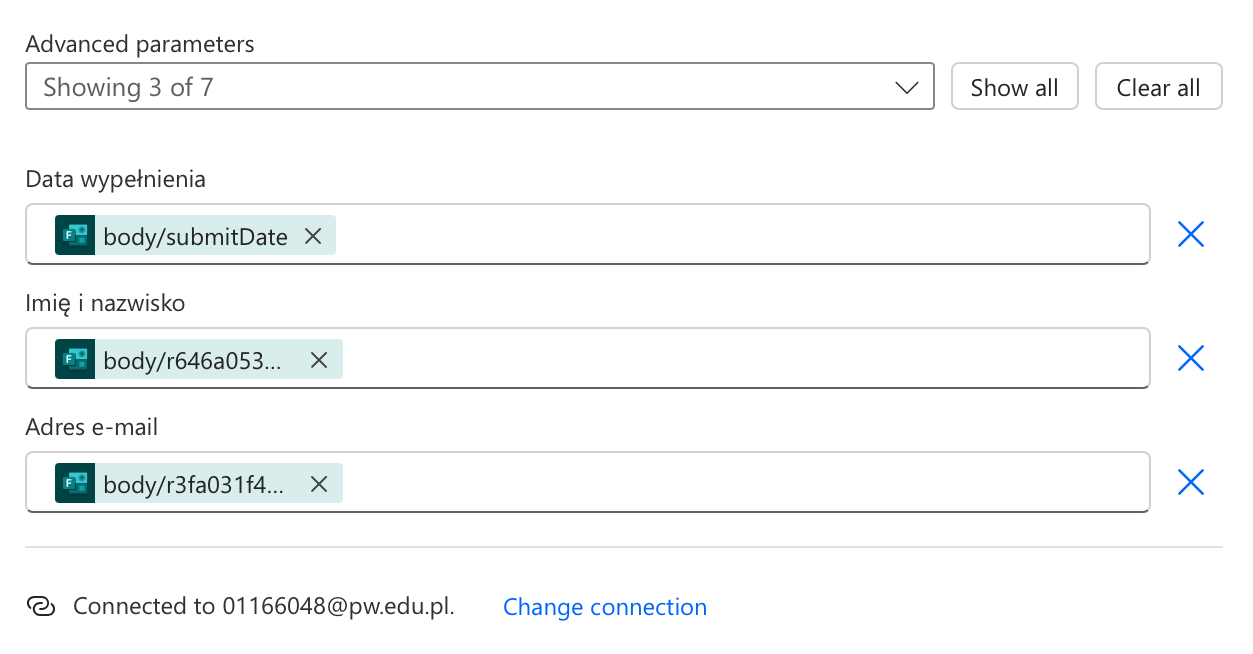
\includegraphics[width=0.7\linewidth]{rysunki/DodanieWierszaAdvanced.png}
	\caption{Zaawansowane parametry konfiguracji ładowania danych do nowego wiersza Microsoft Excel z użyciem Power Automate Flow, źródło: opracowanie własne z użyciem narzędzia \gls{powerautomate}}
\end{figure}

Cały ten proces jest zakodowany w przedstawionym poniżej fragmencie konfiguracji JSON, który został automatycznie wygenerowany na podstawie wizualnych wyborów administratora w interfejsie \gls{powerautomate}. 

\begin{lstlisting}[language=json, caption={Konfiguracja przesyłu danych uczestników do Microsoft Excel z użyciem Power Automate w języku JSON źródło: kod wygenerowany na podstwie konfiguracji poprzez narzędzie Power Automate}]
{
  "type": "OpenApiConnection",
  "inputs": {
    "parameters": {
      "source": "sites/wutwaw.sharepoint.com,7b015f66-4440-4279-bd7d-4c3bd72
      a8931,0e0393fb-6d03-4283-a081-6ec2b7038574",
      "drive": "b!Zl8Be0BEeUK9fUw71yqJMfuTAw4DbYNCoIFuwrcDhXTgMT7sGhSoQ5bE7
      X0hmj-I",
      "file": "01LCUGMVPW6OFHMRQPFVCLYQOK2IH7ACRI",
      "table": "{F5EC12A3-50AA-41BF-834D-21E3EA8E22A8}",
      "item/Data wypelnienia": "@outputs('Pobierz_szczegoly_odpowiedzi')?
      ['body/submitDate']",
      "item/Imie i nazwisko": "@outputs('Pobierz_szczegoly_odpowiedzi')?
      ['body/r646a053d893e4a02be72a3f3150f89be']",
      "item/Adres e-mail": "@outputs('Pobierz_szczegoly_odpowiedzi')?
      ['body/r3fa031f484ed42afb455515c030b4054']"
    },
    "host": {
      "apiId": "/providers/Microsoft.PowerApps/apis/shared_excelonlinebusin
      ess",
      "connection": "shared_excelonlinebusiness-1",
      "operationId": "AddRowV2"
    }
  },
  "runAfter": {
    "Pobierz_szczegoly_odpowiedzi": [
      "Succeeded"
    ]
  },
  "metadata": {
    "01LCUGMVPW6OFHMRQPFVCLYQOK2IH7ACRI": "/Sciencepreneurs Club/Rejestracja/SC BAZA.xlsx",
    "operationMetadataId": "32bed134-874d-48d6-9a14-1e98fdbd233f",
    "tableId": "{F5EC12A3-50AA-41BF-834D-21E3EA8E22A8}"
  }
}
\end{lstlisting}

Przedstawiony fragment kodu określa, w jaki sposób dane z formularza zostaną zapisane w arkuszu \gls{excel}. Typ tego kroku to \texttt{"OpenApiConnection"}, co oznacza standardowe połączenie z usługą \gls{microsoft365}, w tym przypadku z \gls{excel} Online.

W sekcji \texttt{"inputs"} znajdujemy szereg parametrów, które są niezbędne do precyzyjnego zapisania danych. 

Parametr \texttt{"source"} zawiera identyfikator lokalizacji w \gls{sharepoint}, gdzie przechowywany jest plik \gls{excel}. Ten długi ciąg znaków jednoznacznie wskazuje na witrynę \gls{sharepoint} \gls{pw} (wutwaw.sharepoint.com), a kolejne identyfikatory określają dokładną lokalizację w strukturze folderów. 

Parametr \texttt{"drive"} identyfikuje konkretny dysk w \gls{sharepoint}, gdzie znajduje się nasz plik, a \texttt{"file"} wskazuje dokładnie na plik \gls{excel} o nazwie \texttt{"SC BAZA.xlsx"}, co widzimy w sekcji metadanych.

Parametr \texttt{"table"} zawiera unikalny identyfikator tabeli w arkuszu \gls{excel}, do której będziemy dodawać nowy wiersz z danymi uczestnika.
Następnie widzimy serię parametrów definiujących wartości, które zostaną zapisane w poszczególnych kolumnach tabeli. \texttt{"item/Data wypełnienia"} pobiera datę złożenia formularza z poprzedniego kroku \texttt{"item/Imię i nazwisko"} pobiera imię i nazwisko uczestnika \texttt{"item/Adres e-mail"} pobiera adres e-mail. 

Każda z tych wartości jest pobierana z  poprzedniego kroku \texttt{Pobierz\_szczegóły\_odpowiedzi} przy użyciu wyrażenia rozpoczynającego się od \texttt{@outputs}. Wyrażenia te odwołują się do konkretnych pól formularza po ich unikalnych identyfikatorach.

W sekcji \texttt{"host"} widzimy, że używamy \gls{api} Excel Online Business, a operacja to \texttt{"AddRowV2"}, co jednoznacznie wskazuje, że dodajemy nowy wiersz do tabeli.

Element \texttt{"runAfter"} określa, że ten krok zostanie wykonany tylko po pomyślnym zakończeniu kroku \texttt{"Pobierz\_szczegóły\_odpowiedzi"}. Jest to logiczne zabezpieczenie - system najpierw musi pobrać dane z formularza, zanim będzie mógł je zapisać w Excelu.

Sekcja \texttt{"metadata"} zawiera dodatkowe informacje, w tym ścieżkę do pliku \gls{excel} \texttt{"/Sciencepreneurs Club/Rejestracja/SC BAZA.xlsx"} oraz identyfikatory używane przez system do śledzenia operacji.

Warto zauważyć, że choć kod zawiera wiele technicznych szczegółów, administrator tworzy ten krok w prosty sposób - wybierając akcję \texttt{"Add a row into a table"} w \gls{excel}, wskazując lokalizację pliku i tabeli, a następnie mapując pola formularza do odpowiednich kolumn w tabeli. \gls{powerautomate} automatycznie generuje cały ten kod na podstawie wizualnych wyborów użytkownika.

Po wykonaniu tego kroku, dane uczestnika są bezpiecznie zapisane w bazie \gls{excel}, gotowe do dalszego wykorzystania przez zespół organizacyjny Sciencepreneurs Club. Dzięki temu zautomatyzowanemu procesowi, administrator nie musi ręcznie eksportować danych z \gls{forms} do \gls{excel}, eliminując potencjalne błędy ludzkie i oszczędzając cenny czas.


\section{Warstwa danych i analizy - Microsoft Excel z Power Query}

\gls{excel} jako narzędzie do przechowywania i analizy danych w systemie Sciencepreneurs Club stanowi rozwiązanie będące kompromisem między praktycznością a optymalnymi praktykami zarządzania danymi. Wybór ten, choć niepozbawiony ograniczeń technicznych, odzwierciedla realia organizacyjne i zasobowe \gls{inin}, gdzie priorytetem było szybkie wdrożenie systemu w ramach istniejącej infrastruktury \gls{microsoft365}.

Plik \gls{excel} \texttt{"SC BAZA.xlsx”} pełni rolę centralnej bazy danych, w której przechowywane są informacje o wszystkich uczestnikach programu. Znajduje się on na \gls{onedrive} \gls{pw} na kanale \gls{inin} \texttt{"Inkubator\_PW"} w folderze Sciencepreneurs Club. Składa się z kilku kluczowych arkuszy:

\begin{itemize}
    \item \textbf{Baza (unikatowi uczestnicy)} – lista unikalnych uczestników i liczba edycji, w których wzięli udział.
    \item \textbf{Baza} – główna lista wszystkich rejestracji uczestników w poszczególnych edycjach.
    \item \textbf{Uczestnicy \#1, Uczestnicy \#2, Uczestnicy \#3} – arkusze dedykowane każdej edycji Sciencepreneurs Club. Z każdą nową edycją liczba arkuszy będzie rosła analogicznie. Dzięki temu dane z poszczególnych edycji są łatwo dostępne. To do tych arkuszy trafiają dane zebrane z rejestracji online za pomocą formularza \gls{forms}. 
\end{itemize}

Przy analizie warstwy danych i analizy wykorzystującej \gls{excel} z \gls{powerquery} w systemie Sciencepreneurs Club, istotnym elementem jest omówienie aspektów bezpieczeństwa i zarządzania dostępem. 

Wybór \gls{excel} jako głównej bazy danych, choć uzasadniony w kontekście organizacyjnym, niesie jednak ze sobą szereg ograniczeń i wyzwań, które należy świadomie adresować.

\begin{itemize}
\item \textbf{Granularność uprawnień} – Excel nie pozwala na definiowanie uprawnień na poziomie poszczególnych rekordów czy kolumn. Dostęp jest kontrolowany na poziomie całego pliku lub, w ograniczonym zakresie, na poziomie arkuszy poprzez ich blokowanie. \cite{microsoft_excel_blocking_2025}
\item \textbf{Śledzenie zmian} – choć \gls{onedrive}/\gls{sharepoint} oferuje historię wersji, nie dorównuje ona funkcjonalności integralności referencyjnej (każda wartość klucza obcego w jednej tabeli odnosi się do istniejącego rekordu w tabeli nadrzędnej) ani transakcyjnej, co oznacza, że użytkownicy mogą wprowadzać niespójne dane, dostępnych w systemach \gls{sql}, co utrudnia audyt zmian. \cite{microsoft_office_versions_2025}
\item \textbf{Ryzyko nieautoryzowanych modyfikacji} – każdy użytkownik z uprawnieniami edycji może potencjalnie zmodyfikować nie tylko dane, ale również strukturę arkuszy czy formuły \gls{powerquery}, co stanowi istotne ryzyko dla integralności danych. \cite{Microsoft365Groups2025}
\item \textbf{Brak walidacji na poziomie komórek} – \gls{excel} nie oferuje równie zaawansowanych mechanizmów walidacji jak systemy \gls{dbms}, co zwiększa ryzyko wprowadzenia niepoprawnych lub niespójnych danych. \cite{microsoft_excel_validation_2025}
\end{itemize}

W systemie Sciencepreneurs Club ograniczenia te są częściowo kompensowane przez warstwę kontroli dostępu oferowaną przez platformę \gls{sharepoint}, gdzie plik jest przechowywany. Dostęp do pliku jest limitowany do członków grupy \gls{inin}, co stanowi pierwszą linię obrony przed nieautoryzowanym dostępem.

Plik \gls{excel} \texttt{"SC BAZA.xlsx"} przechowywany na \gls{onedrive} \gls{pw} w folderze Sciencepreneurs Club na kanale \gls{inin} \texttt{"Inkubator\_PW"} dzięki zaawansowanym standardom bezpieczeństwa \gls{microsoft365} podlega wielopoziomowemu systemowi zabezpieczeń. \cite{Microsoft365Groups2025}

\begin{itemize}
    \item \textbf{Brak dostępu zewnętrznego} - w obecnej konfiguracji plik nie jest udostępniany użytkownikom spoza domeny \gls{pw}. \cite{Microsoft365Groups2025}
    \item \textbf{Uwierzytelnianie dwuskładnikowe} - dostęp do pliku wymaga logowania do konta \gls{pw}, które może być dodatkowo zabezpieczone przez uwierzytelnianie dwuskładnikowe. \cite{kastwal2023}
    \item \textbf{Kontrola dostępu na poziomie \gls{sharepoint}/\gls{onedrive}} - dostęp do pliku jest ograniczony do członków grupy \gls{inin} oraz administratorów platformy. Uprawnienia są dziedziczone z nadrzędnej struktury folderów, zapewniając spójny model bezpieczeństwa. \cite{Microsoft365Groups2025}
    \item \textbf{Historia wersji} - \gls{onedrive} automatycznie przechowuje wcześniejsze wersje dokumentu, umożliwiając odzyskanie danych w przypadku nieautoryzowanych zmian lub uszkodzenia pliku. \cite{microsoft_office_versions_2025}
\end{itemize}

Excel jako narzędzie do przechowywania danych posiada pewne ograniczenia wydajnościowe, które teoretycznie mogłyby wpływać na funkcjonowanie systemu. \gls{excel}posiada ograniczenie limitów pojemności do 1 048 576 wierszy na arkusz.\cite{microsoft_excel_specs_2025} Złożone transformacje \gls{powerquery} mogą wpływać na wydajność, responsywność pliku.

W kontekście Sciencepreneurs Club, prawdopodobieństwo przekroczenia tych limitów jest jednak znikome. Biorąc pod uwagę skalę wydarzenia (kilkadziesiąt do maksymalnie kilkuset uczestników per edycja) oraz częstotliwość organizacji (kilka edycji rocznie), system mógłby funkcjonować przez wiele lat bez zbliżania się do technicznych ograniczeń \gls{excel}. Nawet przy ambitnym założeniu rozwoju inicjatywy, liczba zapisów w bazie prawdopodobnie nie przekroczyłaby kilkudziesięciu tysięcy w perspektywie długoterminowej, co stanowi zaledwie ułamek możliwości \gls{excel}.

Dlatego, choć świadomość tych ograniczeń jest istotna z perspektywy projektowej, nie stanowią one realnego zagrożenia dla funkcjonalności systemu w przewidywalnej przyszłości.

\gls{powerquery} pełni w systemie rolę zbliżoną do silnika zapytań w tradycyjnych bazach danych, umożliwiając transformację, filtrowanie i agregację danych bez konieczności pisania skomplikowanych formuł w arkuszach. Ta funkcjonalność w istotny sposób kompensuje niektóre ograniczenia \gls{excel} jako bazy danych. Wykorzystując \gls{powerquery} w tym projekcie eliminowane są duplikaty, scalane arkusze edycji oraz generowane zestawienia statystyczne. Dane w arkuszach są przetwarzane w kilku etapach. \cite{microsoft_power_query_2025}

Pierwszym krokiem jest pobranie danych z poszczególnych arkuszy \gls{excel}. W pliku Sciencepreneurs Club BAZA.xlsx znajdują się arkusze zawierające informacje o różnych edycjach programu. \gls{powerquery} dynamicznie wczytuje je jako źródła danych.

\begin{lstlisting}[language=PowerQueryM, caption=Kod ładowania arkusza do Power Query w języku M źródło: opracowanie własne]
Source = Excel.CurrentWorkbook(){[Name="Baza"]}[Content]
\end{lstlisting}

Powyższa funkcja pobiera zawartość tabeli o nazwie Baza z bieżącego skoroszytu.

Nie wszystkie kolumny w pobranym źródle są potrzebne do dalszej analizy. \gls{powerquery} pozwala na ich usunięcie, aby uprościć przetwarzanie.

\begin{lstlisting}[language=PowerQueryM, caption=Kod usuwania niepotrzebnych kolumn w Power Query w języku M źródło: opracowanie własne]
UsunieteKolumny = Table.RemoveColumns(Source,{"Kolumna1", "Kolumna2"})
\end{lstlisting}
Tutaj usunięte zostają zbędne kolumny Kolumna1 i Kolumna2, co ułatwia dalsze operacje.

Aby uzyskać listę unikalnych uczestników, \gls{powerquery} wykorzystuje funkcję Table.Distinct, która eliminuje powtarzające się wpisy na podstawie wybranych kolumn.

\begin{lstlisting}[language=PowerQueryM, caption=Kod usuwania duplikatów – tworzenie listy unikalnych uczestników w Power Query w języku M źródło: opracowanie własne]
UnikalneWpisy = Table.Distinct(Source, {"Imie", "Nazwisko", "Adres e-mail"})
\end{lstlisting}
Ten krok zapewnia, że każdy uczestnik pojawia się tylko raz w bazie głównej.

Ponieważ w bazie mamy dane z różnych edycji Sciencepreneurs Club, konieczne jest ich scalanie. W \gls{powerquery} służy do tego funkcja Table.Combine.

\begin{lstlisting}[language=PowerQueryM, caption=Kod scalający dane z różnych edycji w Power Query w języku M źródło: opracowanie własne]
PolaczoneEdycje = Table.Combine({Edycja1, Edycja2, Edycja3})
\end{lstlisting}

\gls{powerquery} pobiera dane z kilku tabel (np. Edycja1, Edycja2, Edycja3) i łączy je w jedną spójną tabelę.

Dane pochodzące z formularzy \gls{forms} mają format tekstowy, nawet jeśli zawierają liczby lub daty. \gls{powerquery} pozwala na konwersję typów danych:

\begin{lstlisting}[language=PowerQueryM, caption=Kod zmieniający formaty danych w Power Query w języku M źródło: opracowanie własne]
ZmianaTypow = Table.TransformColumnTypes(PolaczoneEdycje,
  {{"Data rejestracji", type date}, {"Liczba edycji", Int64.Type}})
})
\end{lstlisting}
Data rejestracji zostaje skonwertowana na format daty.
Liczba edycji zostaje zmieniona na format liczbowy całkowity (Int64).

W kolejnym kroku \gls{powerquery} liczy, ile razy dany uczestnik wziął udział w różnych edycjach programu. Służy do tego funkcja Table.Group.

\begin{lstlisting}[language=PowerQueryM, caption=Kod grupujący i liczący udział uczestnika w Power Query w języku M źródło: opracowanie własne]
Podsumowanie = Table.Group(PolaczoneEdycje, 
  {"Imie", "Nazwisko", "Adres e-mail"},
  {{"Liczba edycji", each Table.RowCount(_), type number}})
\end{lstlisting}

Dane są grupowane według imienia, nazwiska i adresu e-mail.
Dla każdej grupy \gls{powerquery} liczy liczbę wystąpień danej osoby w różnych edycjach.

Aby wzbogacić bazę główną o dodatkowe informacje, \gls{powerquery} scala tabele na podstawie kluczowych kolumn.

\begin{lstlisting}[language=PowerQueryM, caption=Kod scalający dane z bazą uczestników w Power Query w języku M źródło: opracowanie własne]
ScalonaTabela = Table.NestedJoin(UnikalneWpisy, "Adres e-mail", Podsumowanie, "Adres e-mail", "DaneEdytowane", JoinKind.LeftOuter)
\end{lstlisting}

Tabela UnikalneWpisy jest łączona z Podsumowanie na podstawie adresu e-mail.
Do głównej tabeli dodajemy informację o liczbie edycji, w których uczestniczyła dana osoba.

Dzięki temu \gls{excel} nie jest tylko statycznym arkuszem kalkulacyjnym, ale dynamicznym narzędziem do analizy danych.

Mimo omówionych ograniczeń, wybór \gls{excel} z \gls{powerquery} jako centralnej bazy danych systemu Sciencepreneurs Club niesie ze sobą szereg istotnych korzyści.
Niska bariera wejścia nie wymaga specjalistycznej wiedzy z zakresu baz danych do zarządzania systemem. Jest szczególnie istotne w kontekście studenckiej inicjatywy o rotacyjnym zespole administracyjnym.
\gls{excel} dzięki integracja z ekosystemem \gls{microsoft365} płynnie współpracuje z pozostałymi komponentami systemu (\gls{forms}, \gls{powerautomate}), eliminując potrzebę dodatkowych interfejsów integracyjnych.
Wykorzystanie istniejącej infrastruktury i licencji pozwoliło na szybkie wdrożenie systemu bez dodatkowych kosztów i procedur administracyjnych.
Struktura oparta na arkuszach \gls{excel} umożliwia łatwe dostosowywanie systemu do zmieniających się potrzeb bez konieczności modyfikacji schematów bazy danych.

Te zalety, w połączeniu z automatyzacją oferowaną przez \gls{powerquery}, tworzą rozwiązanie, które, mimo swoich technicznych ograniczeń, jest dobrze dopasowane do skali i charakteru projektu Sciencepreneurs Club.

Przyjęte rozwiązanie, zawiera również potencjał do przyszłej ewolucji i migracji, gdy ograniczenia \gls{excel} staną się bardziej odczuwalne. Obecna modułowa architektura danych, z wyraźnym rozdzieleniem na unikalne encje (uczestnicy) i zdarzenia (rejestracje), ułatwia potencjalną migrację do relacyjnej bazy danych. Zautomatyzowane, standaryzowane przepływy pracy ustanowione w obecnym systemie mogą być relatywnie łatwo przeniesione do bardziej zaawansowanej infrastruktury. Projekt może ewoluować w kierunku hybrydowego rozwiązania w momencie migracji do bardziej zaawansowanego systemu przechowywania danych, gdzie \gls{excel} pełni funkcję interfejsu użytkownika.

Dzięki wykorzystaniu \gls{powerquery} jako warstwy abstrakcji nad strukturą przechowywania danych, przyszłe zmiany w backendzie systemu będą mogły być wprowadzane z minimalnym wpływem na istniejące procesy i doświadczenie użytkownika.

Warto podkreślić, że decyzja o wykorzystaniu \gls{excel} jako bazy danych nie była motywowana wyłącznie technicznymi zaletami tego rozwiązania, ale przede wszystkim realiami organizacyjnymi i zasobowymi \gls{inin}, gdzie priorytetem było szybkie wdrożenie funkcjonalnego systemu w ramach istniejącej infrastruktury. Ta pragmatyczna perspektywa jest istotnym aspektem inżynierii oprogramowania w rzeczywistych warunkach organizacyjnych, gdzie optymalne rozwiązania techniczne muszą być często równoważone z praktycznymi ograniczeniami.

\chapter{Analiza efektywności}
Wdrożenie zautomatyzowanego systemu przetwarzania danych w projekcie Sciencepreneurs Club ma na celu usprawnienie zarządzania rejestracją uczestników i analizą frekwencji. Sama implementacja nowych narzędzi to jednak dopiero początek – kluczowe jest określenie, czy rzeczywiście przyniosły one oczekiwane korzyści. Czy automatyzacja pozwoliła wyeliminować błędy i skrócić czas pracy? Jak ocenia ją administrator systemu? Czy koszty wdrożenia były uzasadnione w kontekście osiągniętych usprawnień? Aby odpowiedzieć na te pytania, przeprowadzono analizę efektywności, obejmującą zarówno aspekty operacyjne, jak i ekonomiczne. Ocenie została poddana jakość przetwarzania danych, wpływ systemu na organizację pracy oraz poziom automatyzacji w porównaniu do wcześniejszego rozwiązania. Dodatkowo przeanalizowane zostały koszty wdrożenia i utrzymania systemu, aby określić, na ile inwestycja w automatyzację jest opłacalna.

\section{Analiza ilościowa i jakościowa}

Podstawowym wskaźnikiem jest dokładność i kompletność danych. W celu zweryfikowania, czy nowe operacje automatyzacji nie wpływają na utratę lub błędne przetwarzanie rekordów, przeprowadzono szczegółowe porównanie danych. Test jakości danych polegał na trzech krokach. Pierwszy, po zakończeniu rejestracji dla danej edycji generowano zrzut danych bezpośrednio z formularza Microsoft Forms. W pierwotnym systemie dane te były zawsze kompletne (100\% poprawnych rekordów). W drugim kroku zrzut danych z Forms został porównany z danymi załadowanymi do arkusza \gls{excel}, który stanowił bazę przetwarzania w nowym systemie. Porównano rekordy na podstawie kluczowych pól (np. adres e-mail, imię, nazwisko). Następnie dane z arkusza Excel zostały porównane z główną bazą unikatowych uczestników oraz bazą frekwencji. Celem było sprawdzenie, czy każdy rekord z edycji (wraz z ewentualnymi korektami, np. dodanym wpisem uczestnika, który pojawił się bez wcześniejszego zgłoszenia) został prawidłowo zintegrowany w centralnej bazie. Dzięki tej metodzie badawczej możliwe było ilościowe potwierdzenie, że nowa automatyzacja nie wpływa negatywnie na integralność danych, a przetwarzanie przebiega zgodnie z oczekiwaniami. W rezultacie wskaźnik poprawności danych wyniósł 100\%, co potwierdza, że żaden rekord nie został utracony ani błędnie przetworzony w procesie automatyzacji.

Kiedy już wiarygodność danych została potwierdzona, kluczowym wskaźnikiem sukcesu systemu jest ocena administratora. Choć proces rejestracji nie ulega zmianie z perspektywy uczestników, administrator będzie odczuwał  różnicę, ponieważ jego zakres pracy ulegnie zmianie. Jako osoba odpowiedzialna za zarządzanie systemem, administrator dysponuje unikalnym wglądem w jego wydajność, użyteczność oraz stabilność. Do oceny wykorzystano ankietę satysfakcji z użyciem 5-punktowej skali Likerta (1 – niezadowolony, 5 – bardzo zadowolony).

\begin{table}[ht]
    \centering
    \renewcommand{\arraystretch}{1.3} % Zwiększenie odstępów między wierszami
    \caption[Ocena administratora systemu bazowego i zautomatyzowanego, źródło: opracowanie własne]{Ocena administratora systemu bazowego i zautomatyzowanego}
    \begin{tabular}{| p{4cm} | p{5cm} | p{5cm} |}
        \hline
        \textbf{Kategoria} & \textbf{Bazowy system} & \textbf{Zautomatyzowany system} \\
        \hline
        \textbf{Ocena administratora} & Średnia ocena: 3,5/5 & Średnia ocena: 4,8/5 \\
        \hline
    \end{tabular}
    \vspace{0.5em}
    \par\raggedright\footnotesize{Źródło: opracowanie własne}
\end{table}

Agnieszka Lewandowska, administrator systemu, wyraziła bardzo wysoką satysfakcję (4,8/5). W wywiadzie podkreśliła: „Instrukcja krok po kroku i film instruktażowy pozwoliły mi przygotować kolejną edycję bez problemów. System działa niezawodnie, a Power Query automatycznie usuwa duplikaty i aktualizuje raporty.”

Ocenie został poddany również czas przetwarzania danych, który odpowiada za efektywność całego systemu. Czas przetwarzania danych obejmuje zarówno setup nowej edycji, jak i analizę bieżących zgłoszeń. Główną zmianą jest kolejność zadań wykonywanych przez administratora. W pierwszej edycji przetwarzanie danych oraz ich analiza były manualnym procesem wykonywanym po wydarzeniu, teraz przed rejestracją uczestników administrator aktualizuje system na kolejną edycję Sciencepreneurs Club, a przetwarzanie i analiza odbywają się automatycznie. W poprzednim analiza frekwencji trwała czasem pół dnia (identyfikacja osób uczestniczących w więcej niż jednym spotkaniu, a następnie sporządzenie listy unikalnych uczestników i przypisanie każdemu z nich frekwencji), dodatkowo była narażona na manualne błędy. W nowym systemie lista jest aktualizowana na bieżąco, co umożliwia natychmiastową analizę i szybką reakcję na zmieniające się warunki przed wydarzeniem. 

\begin{table}[ht]
    \centering
    \renewcommand{\arraystretch}{1.3} % Zwiększenie odstępów między wierszami
    \caption[Porównanie czasu pracy systemu bazowego i zautomatyzowanego, źródło: opracowanie własne]{Porównanie czasu pracy systemu bazowego i zautomatyzowanego}
    \begin{tabular}{| p{4cm} | p{5cm} | p{5cm} |}
        \hline
        \textbf{Kategoria} & \textbf{Bazowy system} & \textbf{Zautomatyzowany system} \\
        \hline
        Setup nowej edycji & 20 min (Forms) & 40 min (Forms, Power Automate, Power Query) \\
        \hline
        Przetwarzanie zgłoszeń & 2 godziny (automatyczna synchornizacja + ewentualne manualne uzupełnienia uczestnków) & Automatyczne (automatyczna synchronizacja + automatyczne uzupełnienie uczestników podczas wydarzenia) \\
        \hline
        Analiza frekwencji & 4 godziny (ręczne opracowanie) & Automatyczna, z możliwością drobnych korekt \\
        \hline
    \end{tabular}
    \vspace{0.5em}
    \par\raggedright\footnotesize{Źródło: opracowanie własne}
\end{table}

Choć setup nowej edycji (obejmujący konfigurację \gls{powerautomate}, \gls{powerquery} i \gls{forms} trwa około godzinę, całościowy czas przetwarzania zgłoszeń oraz generowania raportów został skrócony do kilku godzin, a automatyzacja raportowania (np. analiza frekwencji) odbywa się w tle, eliminując potrzebę manualnych interwencji.

W analizie porównano stopień automatyzacji systemu przed i po wdrożeniu rozwiązań automatyzujących. W systemie bazowym, gdzie większość operacji, weryfikacja i przetwarzanie danych oraz późniejsze analizy frekwencji były wykonywane ręcznie, stopień automatyzacji oceniono na około 12,5\%. Na podstawie zmapowania każdego etapu pracy, gdzie jedynie pobranie danych z \gls{forms} do \gls{excel} odbywało się automatycznie, tylko 1/8 etapów nie wymagała manualnej interwencji. Pozostałe etapy to: przygotowanie formularza \gls{forms}, publikacja formularza rejestracyjnego, wydrukowanie tabel z dodatkowymi miejscami na wpisy, uzupełnienie ewentualnie dopisanych uczestników na miejscu, identyfikacja osób uczestniczących w więcej niż jednym spotkaniu, a następnie sporządzenie listy unikalnych uczestników i przypisanie każdemu z nich frekwencji. Oznacza to, że większość zadań wymagała bezpośredniej interwencji administratora, co nie tylko wydłużało czas obsługi, ale również zwiększało ryzyko wystąpienia błędów. 
Wdrożenie zautomatyzowanego systemu, opartego na narzędziach takich jak \gls{powerautomate} i \gls{powerquery}, umożliwiło automatyzację kluczowych procesów. Dodatkowa rezygnacja z ręcznego dopisywania uczestników w dniu wydarzenia na rzecz przekierowania ich do rejestracji online skróciła czas pracy i zmniejszyła podatność na błędy. Dzięki temu przepływy pracy zostały znacząco usprawnione, co pozwoliło na ograniczenie ręcznych interwencji i skrócenie czasu realizacji zadań do około 50\% automatyzacji, gdzie 4/8 etapów odbywa się bez manualnej pracy. Usunięto ręcznie dodawane etapy obsługi uczestników, w zamian wprowadzono dodatkowe czynności manualne związane z konfiguracją, jednak przetwarzanie danych odbywa się w pełni automatycznie. Taka zmiana wpływa korzystnie zarówno na efektywność operacyjną, jak i na poprawę jakości danych.

\begin{table}[ht]
    \centering
    \caption[Porównanie stopnia automatyzacji systemu bazowego i zautomatyzowanego, źródło: opracowanie własne]{Porównanie stopnia automatyzacji systemu bazowego i zautomatyzowanego}
    \renewcommand{\arraystretch}{1.3} % Zwiększenie odstępów między wierszami
    \begin{tabular}{| l | c | c |}
        \hline
        \textbf{Kategoria} & \textbf{Bazowy system} & \textbf{Zautomatyzowany system} \\
        \hline
        \textbf{Stopień automatyzacji} & 12,5\% & 50\% \\
        \hline
    \end{tabular}
    \vspace{0.5em}
    \par\raggedright\footnotesize{Źródło: opracowanie własne}
\end{table}

Transformacja systemu umożliwiła znaczną redukcję manualnych operacji, co przekłada się na wyższą wydajność i mniejsze ryzyko błędów. 

\section{Szczegółowa analiza kosztów wdrożenia}
W celu efektywnej realizacji projektu wdrożenia systemu automatyzacji rejestracji uczestników wydarzeń w ramach \gls{pw} przeprowadzono szczegółową analizę budżetową. Przygotowane zestawienie kosztów posłużyło jako podstawa do podjęcia decyzji przez kierownictwo \gls{inin}, zapewniając przejrzystość finansowania oraz uwzględniając dostępne środki uczelni.

Projekt finansowany jest w całości ze środków uczelni, bez konieczności pozyskiwania dodatkowych funduszy zewnętrznych. Kluczowe źródła finansowania to budżet operacyjny \gls{cinn}, przeznaczony na wynagrodzenia pracowników oraz licencje \gls{microsoft365}, pokrywające koszty wykorzystania narzędzi \gls{excel}, \gls{powerautomate} i \gls{forms}, co eliminuje konieczność ponoszenia dodatkowych opłat licencyjnych. Alokacja środków odbywa się w ramach rocznego budżetu jednostki, przy czym projekt realizowany jest w obrębie programu optymalizacji procesów administracyjnych, stanowiącego jeden z elementów strategii cyfryzacji uczelni.

Koszty wdrożenia obejmują wszystkie niezbędne nakłady na realizację projektu, w tym wynagrodzenia zespołu oraz dodatkowe koszty związane z implementacją.

\begin{table}[ht]
    \centering
    \caption[Koszty personelu w projekcie wdrożenia, źródło: opracowanie własne na podstawie danych kadrowych ININ]{Koszty personelu w projekcie wdrożenia}
    \renewcommand{\arraystretch}{1.3} % Zwiększenie odstępów między wierszami
   \begin{tabular}{| p{2,3cm} | p{5cm} | p{3cm} | p{3,5cm} |}
        \hline
        \textbf{Stanowisko} & \textbf{Miesięczne wynagrodzenie (PLN)} & \textbf{Alokacja czasu} & \textbf{Koszt w projekcie (PLN)} \\
        \hline
        Praktykantka & 6 000 & 60\% $\times$ 1 miesiąc & 3 600 \\
        \hline
        Kierownik projektu & 13~600 & 10\% $\times$ 1 miesiąc & 1 360 \\
        \hline
        \textbf{Suma} & & & \textbf{4~960} \\
        \hline
    \end{tabular}
    \vspace{0.5em}
    \par\raggedright\footnotesize{Źródło: opracowanie własne na podstawie danych kadrowych ININ}
\end{table}


Analiza kosztów personelu opiera się na rzeczywistych stawkach wynagrodzenia pracowników \gls{inin} oraz na precyzyjnie oszacowanym czasie poświęconym na realizację projektu. Kluczowym założeniem jest zaangażowanie praktykantki w wymiarze 60\% miesięcznego czasu pracy (co odpowiada około 96 godzinom) oraz kierownika projektu w wymiarze 10\% (około 16 godzin).

Wybór takiej struktury zespołu projektowego jest nieprzypadkowy – praktykantka posiada niezbędne kompetencje techniczne do implementacji systemu, natomiast kierownik projektu zapewnia nadzór merytoryczny, koordynację działań oraz podejmowanie kluczowych decyzji. Alokowanie do projektu doświadczonego kierownika jedynie w niezbędnym wymiarze czasu (10\%) jest przykładem efektywnego zarządzania zasobami ludzkimi, co przełożyło się na redukcję kosztów personalnych o około 30\% w porównaniu do standardowego modelu realizacji, gdzie zaangażowanie kierownika wynosi zwykle około 25-30\% czasu.

\begin{table}[ht]
    \centering
    \caption[Dodatkowe koszty wdrożenia uwzględniające czas uczestników, źródło: opracowanie własne]{Dodatkowe koszty wdrożenia uwzględniające czas uczestników}
    \label{tab:dodatkowe_koszty_czas}
    \renewcommand{\arraystretch}{1.3} % Zwiększenie odstępów między wierszami
    \begin{tabular}{| p{0.30\textwidth} | p{0.20\textwidth} | p{0.15\textwidth} | p{0.20\textwidth} |}
        \hline
        \textbf{Kategoria} & \textbf{Szczegóły} & \textbf{Koszt (PLN)} & \textbf{Uzasadnienie} \\
        \hline
        Uczestnictwo w~szkoleniach & Czas zespołu ININ (5 osób) & 1~500 & 5 osób $\times$ 3h $\times$ 100 PLN/h \\
        \hline
        \textbf{Suma} & & \textbf{1~500} & \\
        \hline
    \end{tabular}
    \vspace{0.5em}
    \par\raggedright\footnotesize{Źródło: opracowanie własne}
\end{table}

Dodatkowe koszty, często bywają pomijane w podstawowych analizach ekonomicznych. W przedstawionej tabeli uwzględniono koszty czasu poświęconego przez uczestników szkolenia, którzy nie są bezpośrednio zaangażowani w realizację projektu.
W szkoleniu uczestniczyło 5 osób z zespołu \gls{inin}, a każda z nich poświęciła na to 3 godziny swojego czasu pracy. Przyjmując średnią stawkę godzinową na poziomie 100 zł/h (odpowiadającą typowym kosztom pracy specjalistów w \gls{inin}), uzyskujemy łączny koszt 1 500 zł. Uwzględnienie tego kosztu jest kluczowe dla rzetelnej oceny całkowitych nakładów związanych z wdrożeniem, gdyż czas poświęcony na szkolenia to czas, który mógłby zostać wykorzystany na inne zadania operacyjne.

\begin{table}[ht]
    \centering
    \caption[Całkowite koszty wdrożenia, źródło: opracowanie własne]{Zestawienie całkowitych kosztów wdrożenia}
    \label{tab:calkowite_koszty_wdrozenia}
    \renewcommand{\arraystretch}{1.3} % Zwiększenie odstępów między wierszami
    \begin{tabular}{| p{0.5\textwidth} | r |}
        \hline
        \textbf{Kategoria kosztów} & \textbf{Wartość (PLN)} \\
        \hline
        Koszty personelu & 4~960 \\
        \hline
        Koszty uczestnictwa w szkoleniach & 1~500 \\
        \hline
        \textbf{Suma} & \textbf{6~460} \\
        \hline
    \end{tabular}
    \vspace{0.5em}
    \par\raggedright\footnotesize{Źródło: opracowanie własne}
\end{table}

Zestawienie całkowitych kosztów wdrożenia pozwala na kompleksową ocenę nakładów finansowych niezbędnych do realizacji projektu. Całkowity koszt w wysokości 6 460 zł stanowi sumę kosztów personelu 4 960 zł oraz kosztów uczestnictwa w szkoleniach 1 500 zł.

Ta wartość reprezentuje rzeczywisty, całościowy koszt wdrożenia, uwzględniający zarówno bezpośrednie koszty implementacji systemu, jak i niezbędne koszty dodatkowe wynikające z zaangażowania czasu wszystkich uczestników projektu. 

System został zaprojektowany tak, aby utrzymanie automatyzacji rejestracji wymagało minimalnych nakładów finansowych. Ponieważ każda edycja wydarzenia wymaga utworzenia nowego przepływu pracy i formularza, koszty operacyjne zostały skalkulowane w sposób cykliczny.

\begin{table}[ht]
    \centering
    \caption[Koszty operacyjne systemu automatyzacji rejestracji, źródło: opracowanie własne na podstawie kalkulacji z wykorzystaniem \gls{mcc}]{Koszty operacyjne systemu automatyzacji rejestracji}
    \label{tab:koszty_operacyjne_systemu}
    \renewcommand{\arraystretch}{1.3} % Zwiększenie odstępów między wierszami
    \begin{tabular}{| p{0.32\textwidth} | p{2,2cm} | p{1,6cm} | p{0.31\textwidth} |}
        \hline
        \textbf{Kategoria kosztów} & \textbf{Wartość miesięczna (PLN)} & \textbf{Wartość roczna (PLN)} & \textbf{Źródło finansowania} \\
        \hline
        \gls{excel} (baza danych)  & 10 & 120 & W ramach licencji \gls{microsoft365} \\
        \hline
        \gls{powerautomate} (przepływy pracy)  & 20 & 240 & W ramach licencji \gls{microsoft365} \\
        \hline
        \gls{forms} (formularze)  & 5 & 60 & W ramach licencji \gls{microsoft365} \\
        \hline
        Wsparcie techniczne - administrator (4h/miesiąc) & 340 & 4~080 & Budżet operacyjny \gls{cinn} \\
        \hline
        \textbf{Łączny koszt} & \textbf{375} & \textbf{4~500} & \textbf{Finansowanie wewnętrzne} \\
        \hline
    \end{tabular}
    \vspace{0.5em}
    \par\raggedright\footnotesize{Źródło: opracowanie własne na podstawie kalkulacji z wykorzystaniem \gls{mcc}}
\end{table}

Łączny miesięczny koszt operacyjny wynoszący 375 zł przekłada się na roczny koszt w wysokości 4 500 zł, co stanowi około 69,6\% całkowitych kosztów wdrożenia (6 460 zł). 

Dzięki wykorzystaniu posiadanych licencji \gls{microsoft365}, wydatki te nie obejmują dodatkowych kosztów subskrypcyjnych ani serwisowych. Koszty związane z \gls{excel}, \gls{powerautomate} oraz \gls{forms} zostały oszacowane na podstawie kalkulatora kosztów Microsoft, który umożliwia precyzyjne określenie kosztów poszczególnych usług w ramach pakietu \gls{microsoft365}. Wartości te odzwierciedlają proporcjonalne obciążenie tych usług przez system automatyzacji rejestracji, uwzględniając zarówno wykorzystanie zasobów obliczeniowych, jak i przestrzeni dyskowej.

Kategoria "Wsparcie techniczne" obejmuje koszty związane z bieżącą obsługą systemu przez administratora. Po dokładnej analizie zadań administratora ustalono, że realistyczne obciążenie pracą wynosi około 4 godzin miesięcznie i obejmuje:
\begin{itemize}
    \item Tworzenie nowych formularzy i przepływów pracy dla każdego wydarzenia (2h/miesiąc)
    \item Rozwiązywanie problemów technicznych i pomoc użytkownikom (1h/miesiąc)
    \item Okresowe przeglądy systemu i aktualizacje dokumentacji (1h/miesiąc)
\end{itemize}

Przyjmując stawkę godzinową administratora na poziomie 85 zł/h (co odpowiada miesięcznemu wynagrodzeniu około 13 600 zł przy pełnym etacie), miesięczny koszt wsparcia technicznego wynosi 340 zł (4h × 85 zł/h), co przekłada się na roczny koszt 4 080 zł.

\begin{table}[ht]
    \centering
    \caption[Prognoza kosztów utrzymania systemu w perspektywie 3-letniej, źródło: opracowanie własne na podstawie prognoz inflacyjnych \cite{NBP2025}]{Prognoza kosztów utrzymania systemu w perspektywie 3-letniej}
    \renewcommand{\arraystretch}{1.3} % Zwiększenie odstępów między wierszami
    \begin{tabular}{| p{0.2\textwidth} | p{0.2\textwidth} | p{0.5\textwidth} |}
        \hline
        \textbf{Rok} & \textbf{Koszt roczny (PLN)} & \textbf{Uzasadnienie} \\
        \hline
        1(2025) & 4~500 & Standardowe koszty operacyjne \\
        \hline
        2(2026) & 4~721 & Uwzględnienie 4,9\% inflacji \\
        \hline
        3(2027) & 4~881 & Uwzględnienie 3,4\% inflacji \\
        \hline
        \textbf{Suma za 3 lata} & \textbf{14~102} & \textbf{} \\
        \hline
    \end{tabular}
    \vspace{0.5em}
    \par\raggedright\footnotesize{Źródło: opracowanie własne na podstawie prognoz inflacyjnych \cite{NBP2025}}
\end{table}

Długoterminowa analiza kosztów utrzymania jest niezbędna dla pełnego zrozumienia ekonomicznych konsekwencji wdrożenia systemu. Przedstawiona prognoza obejmuje perspektywę trzyletnią, co jest średnim horyzontem czasowym dla analiz ekonomicznych projektów realizowanych przez uczelnie wyższe w Polsce. ~\parencite[s. 293]{paczek2018}

Po uwzględnieniu aktualnych prognoz inflacyjnych NBP (4,9\% dla 2025 r., 3,4\% dla 2026 r.), łączne koszty utrzymania w perspektywie 3-letniej wynoszą 14 102 PLN, co stanowi 218,3\% początkowego kosztu wdrożenia (6 460 PLN). Pomimo wyższych kosztów utrzymania, projekt nadal pozostaje ekonomicznie uzasadniony dzięki znaczącym korzyściom ekonomicznym, które zostaną szczegółowo przeanalizowane w kolejnych sekcjach.

\section{Analiza korzyści ekonomicznych}

Kompleksowa analiza ekonomiczna projektu wymaga nie tylko identyfikacji kosztów, ale przede wszystkim kwantyfikacji korzyści. W niniejszej sekcji przedstawiono szczegółową analizę korzyści ekonomicznych wynikających z wdrożenia systemu automatyzacji rejestracji, uwzględniając zarówno bezpośrednie oszczędności czasowe, jak i korzyści wynikające z redukcji błędów oraz poprawy satysfakcji użytkowników.

Automatyzacja procesów rejestracji uczestników wydarzeń przynosi wymierne oszczędności czasowe, które przekładają się na korzyści finansowe.

\begin{table}[ht]
    \centering
    \caption[Oszczędności czasowe wynikające z wdrożenia systemu, źródło: opracowanie własne na podstawie analizy procesów ININ oraz danych z Tabeli 7.2]{Oszczędności czasowe wynikające z wdrożenia systemu}
    \label{tab:oszczednosci_czasowe}
    \renewcommand{\arraystretch}{1.3} % Zwiększenie odstępów między wierszami
    \begin{tabular}{| p{0.35\textwidth} | p{0.15\textwidth} | p{0.45\textwidth} |}
        \hline
        \textbf{Kategoria} & \textbf{Wartość} & \textbf{Uzasadnienie} \\
        \hline
        Czas obsługi jednego wydarzenia przed automatyzacją & 6,33 godziny & Suma czasów: setup (0,33h), przetwarzanie zgłoszeń (2h) i analiza frekwencji (4h) \\
        \hline
        Czas obsługi jednego wydarzenia po automatyzacji & 0,67 godziny & Tylko czas na setup nowej edycji, pozostałe procesy są automatyczne \\
        \hline
        Oszczędność czasu na jedno wydarzenie & 5,67 godziny & Różnica między czasem przed i po automatyzacji (6,33h - 0,67h) \\
        \hline
        Liczba wydarzeń w roku 2023 & 5 & Dane historyczne \\
        \hline
        Liczba wydarzeń w roku 2024 & 7 & Dane historyczne \\
        \hline
        Prognozowana liczba wydarzeń w roku 2025 & 10 & Prognoza na podstawie trendu wzrostowego \\
        \hline
        Łączna roczna oszczędność czasu & 56,7 godziny & Oszczędność na jedno wydarzenie $\times$ liczba wydarzeń w 2025 roku (5,67h $\times$ 10) \\
        \hline
        Stawka godzinowa administratora & 85 PLN/h & Wynikająca z miesięcznego wynagrodzenia 13~600 PLN przy pełnym etacie \\
        \hline
        Roczna oszczędność finansowa & 4~820 PLN & Łączna oszczędność czasu $\times$ stawka godzinowa administratora (56,7h $\times$ 85 PLN/h) \\
        \hline
    \end{tabular}
    \vspace{0.5em}
    \par\raggedright\footnotesize{Źródło: opracowanie własne na podstawie analizy procesów ININ oraz danych z Tabeli 7.2}
\end{table}

Analiza oszczędności czasowych opiera się na szczegółowym badaniu procesów przed i po automatyzacji, przedstawionym w Tabeli 7.2. Warto zauważyć, że setup nowej edycji wymaga nieco więcej czasu w zautomatyzowanym systemie (40 minut) w porównaniu do systemu bazowego (20 minut), co daje ujemną oszczędność czasu w tej kategorii (-20 minut na jedno wydarzenie). Jednak ta dodatkowa inwestycja czasu jest z nawiązką rekompensowana przez automatyzację pozostałych etapów. Przetwarzanie zgłoszeń, które wcześniej zajmowało 2 godziny, teraz odbywa się automatycznie. Analiza frekwencji, która przed automatyzacją wymagała 4 godzin pracy, obecnie jest wykonywana automatycznie. Łączna oszczędność czasu na jedno wydarzenie wynosi 5,67 godziny (czyli 5 godzin i 40 minut). 

\break
Przy prognozie 10 wydarzeń na rok 2025, wynikającej z analizy trendu wzrostowego z lat 2023-2024, przekłada się to na łączną roczną oszczędność 56,7 godzin pracy administratora. Przyjmując stawkę godzinową administratora na poziomie 85 zł/h, wynikającą z jego miesięcznego wynagrodzenia w wysokości 13 600 zł przy pełnym etacie, roczna oszczędność finansowa wynosi 4 820 zł (56,7h × 85 zł/h).

\begin{table}[ht]
    \centering
    \caption[Prognoza rocznych korzyści ekonomicznych z uwzględnieniem inflacji w perspektywie 3-letniej, źródło: opracowanie własne z uwzględnieniem aktualnych prognoz inflacyjnych \cite{NBP2025} oraz danych z Tabeli 7.9]{Prognoza rocznych korzyści ekonomicznych z uwzględnieniem inflacji w perspektywie 3-letniej}
    \renewcommand{\arraystretch}{1.3} % Zwiększenie odstępów między wierszami
    \begin{tabular}{| p{0.2\textwidth} | p{0.2\textwidth} | p{0.5\textwidth} |}
        \hline
        \textbf{Rok} & \textbf{Oszczędności roczne (PLN)} & \textbf{Uzasadnienie} \\
        \hline
        1(2025) & 4~820 & Oszczędności finansowe \\
        \hline
        2(2026) & 5~056 & Uwzględnienie 4,9\% inflacji \\
        \hline
        3(2027) & 5~228 & Uwzględnienie 3,4\% inflacji \\
        \hline
        \textbf{Suma za 3 lata} & \textbf{15~104} & \textbf{Łączne oszczędności} \\
        \hline
    \end{tabular}
    \vspace{0.5em}
    \par\raggedright\footnotesize{Źródło: opracowanie własne z uwzględnieniem aktualnych prognoz inflacyjnych \cite{NBP2025} oraz danych z Tabeli 7.9}
\end{table}

Zestawienie całkowitych rocznych korzyści ekonomicznych pozwala na kompleksową ocenę wartości generowanej przez system automatyzacji rejestracji w perspektywie wieloletniej. W roku 2025 korzyści ekonomiczne wynoszą 4 820 zł, co stanowi  74,6\% całkowitych kosztów wdrożenia (6 460 zł). W kolejnych latach wartość ta rośnie do 5 056 zł w roku 2026 i 5 228 zł w roku 2027, co daje łączną wartość korzyści w analizowanym okresie na poziomie 15 104 zł.

\section{Analiza opłacalności inwestycji}

W celu kompleksowej oceny efektywności ekonomicznej projektu przeprowadzono analizę opłacalności inwestycji, wykorzystując kluczowe wskaźniki finansowe: \gls{npv} oraz \gls{roi}. Zastosowanie tych miar pozwala na ocenę projektu z uwzględnieniem różnych aspektów efektywności ekonomicznej.

\begin{table}[ht]
    \centering
    \caption[Kalkulacja NPV dla projektu automatyzacji, źródło: opracowanie własne]{Kalkulacja NPV dla projektu automatyzacji}
    \renewcommand{\arraystretch}{1.3} % Zwiększenie odstępów między wierszami
    \begin{tabular}{| c | p{0.1\textwidth} | p{0.1\textwidth} | p{0.3\textwidth} | p{0.2\textwidth} |}
        \hline
        \textbf{Rok} & \textbf{Koszty (PLN)} & \textbf{Korzyści (PLN)} & \textbf{Przepływy pieniężne netto (PLN)} & \textbf{Zdyskontowane przepływy (PLN)} \\
        \hline
        0 & 6~460 & 0 & -6~460 & -6~460 \\
        \hline
        1 & 4~500 & 4~820 & 320 & 224 \\
        \hline
        2 & 5~056 & 5~228 & 172 & 83 \\
        \hline
        3 & 4~885 & 5~291 & 406 & 134 \\
        \hline
        \textbf{Suma} & \textbf{20~562} & \textbf{15~104} & \textbf{-5~458} & \textbf{-5~569} \\
        \hline
    \end{tabular}
    \vspace{0.5em}
    \par\raggedright\footnotesize{Źródło: opracowanie własne}
\end{table}

Przyjęta wartość stopy dyskontowej na poziomie 6\% została ustalona w oparciu o cztery czynniki. Pierwszym z nich jest koszt kapitału jednostek sektora publicznego - w przypadku inwestycji uczelnianych, stopa dyskontowa zazwyczaj odzwierciedla koszt finansowania projektów ze środków publicznych. Zgodnie z rekomendacjami Narodowego Banku Polskiego \cite{NBP2023stopy}, zalecana stopa dyskontowa kształtuje się w przedziale 5,87\% dla lat 2025-2027. Kolejnym czynnikiem jest prognozowana inflacja - zgodnie z projekcjami \cite{NBP2025}, średnioroczna inflacja w Polsce w latach 2025-2027 jest prognozowana na poziomie około 5,87\%. 

Na podstawie tych danych, przyjęto stopę dyskontową na poziomie 6\%, co zapewnia konserwatywne podejście do wyceny przyszłych przepływów pieniężnych i jest zgodne z praktyką rynkową dla projektów o podobnym charakterze i poziomie ryzyka.

\gls{npv} projektu przy przyjętej stopie dyskontowej wynosi -5 569 zł, co wskazuje na brak opłacalności ekonomicznej w przyjętym horyzoncie czasowym. Ujemna wartość \gls{npv} oznacza, że zdyskontowane korzyści finansowe nie przewyższają zdyskontowanych kosztów w analizowanym okresie trzech lat. Wynik ten sugeruje, że projekt nie generuje wystarczających korzyści finansowych, aby uzasadnić jego realizację wyłącznie na podstawie kryteriów ekonomicznych.

{ \footnotesize
\begin{equation}\label{eq:Return on Investment}
\text{ROI} = \frac{\text{Suma korzysci} - \text{Suma kosztow}}{\text{Naklady inwestycyjne}} \times 100\% = \frac{15\,104\ \text{PLN} - 14\,102\ \text{PLN}}{6\,460\ \text{PLN}} \times 100\% = \frac{1\,002\ \text{PLN}}{6\,460\ \text{PLN}} \times 100\% = 15{,}5\%
\end{equation}
\equationcaption{Wzór na obliczenie zwrotu z inwestycji (ROI)}
}

Sposób obliczania \gls{roi} przedstawiono we wzorze 7.1, przy czym uwzględniono sumaryczne korzyści oraz nakłady w horyzoncie trzyletnim. Uzyskana wartość \gls{roi} na poziomie 15,5\% w okresie 3 lat oznacza, że każda zainwestowana złotówka przynosi około 0,16 zł zysku ponad poniesione nakłady w analizowanym okresie. W ujęciu rocznym daje to około 4,9\% rocznie.

Warto zauważyć, że mimo ujemnej wartości \gls{npv}, wskaźnik \gls{roi} przyjmuje wartość dodatnią. Wynika to z faktu, że \gls{roi} nie uwzględnia zmiany wartości pieniądza w czasie (nie dyskontuje przepływów pieniężnych), a jedynie bilansuje nominalne korzyści i koszty.
Uzyskany poziom \gls{roi} można uznać za umiarkowany. W sektorze komercyjnym dla projektów IT typowo oczekuje się ROI na poziomie powyżej 50\% w perspektywie 3-letniej, jednak w sektorze publicznym, gdzie projekty często mają charakter niekomercyjny i służą realizacji celów społecznych, niższe wartości \gls{roi} są akceptowalne.
Biorąc pod uwagę, że głównym celem projektu nie była maksymalizacja korzyści finansowych, a poprawa jakości pracy oraz realizacja celów strategicznych uczelni, uzyskany poziom \gls{roi} można uznać za akceptowalny, szczególnie w połączeniu z istotnymi korzyściami jakościowymi i strategicznymi.

\section{Analiza korzyści jakościowych i strategicznych}

Chociaż standardowe wskaźniki finansowe nie wskazują jednoznacznie na wysoką opłacalność ekonomiczną projektu (ujemne \gls{npv} przy umiarkowanym \gls{roi}), należy rozszerzyć analizę o aspekty, które nie zostały uwzględnione w podstawowych kalkulacjach finansowych.

\begin{table}[ht]
    \centering
    \caption[Korzyści jakościowe z wdrożenia systemu automatyzacji, źródło: opracowanie własne na podstawie wywiadów z administratorem]{Korzyści jakościowe z wdrożenia systemu automatyzacji}
    \renewcommand{\arraystretch}{1.3} % Zwiększenie odstępów między wierszami
    \begin{tabular}{| p{0.3\textwidth} | p{0.6\textwidth} |}
        \hline
        \textbf{Kategoria} & \textbf{Opis korzyści} \\
        \hline
        Poprawa jakości pracy administratora & Eliminacja powtarzalnych, czasochłonnych zadań zwiększa satysfakcję z pracy \\
        \hline
        Dostępność danych w czasie rzeczywistym & Administrator ma natychmiastowy dostęp do aktualnych informacji o uczestnikach, co usprawnia proces decyzyjny \\
        \hline
        Standaryzacja procesu & Ujednolicony i powtarzalny proces rejestracji zapewnia spójność danych między kolejnymi edycjami wydarzeń \\
        \hline
        Możliwość generowania automatycznych raportów & System umożliwia automatyczne tworzenie zestawień frekwencji \\
        \hline
        Redukcja stresu administratora & Eliminacja czasochłonnych, manualnych czynności zmniejsza poziom stresu i ryzyka wypalenia zawodowego \\
        \hline
    \end{tabular}
    \vspace{0.5em}
    \par\raggedright\footnotesize{Źródło: opracowanie własne na podstawie wywiadów z administratorem}
\end{table}

Korzyści jakościowe, choć trudne do bezpośredniej wyceny, mają istotny wpływ na wartość projektu. Szczególnie ważna jest poprawa warunków pracy administratora, który zamiast poświęcać czas na rutynowe, manualne zadania, może skupić się na bardziej wartościowych aspektach organizacji wydarzeń Sciencepreneurs Club. 

Wdrożenie systemu automatyzacji rejestracji wpisuje się w szerszy kontekst strategiczny \gls{pw}, zdefiniowany w dokumencie "Strategia rozwoju Politechniki Warszawskiej do roku 2030" ~\parencite[s. 16]{PW2030}. Projekt ten, choć niewielki w skali uczelni, stanowi istotny element realizacji wizji nowoczesnej instytucji akademickiej, działającej w oparciu o najnowsze technologie i efektywne procesy organizacyjne.

Wdrożony system automatyzacji wpisuje się bezpośrednio w obszar Strategicznego Pola Oddziaływania "Informacja i otoczenie cyfrowe", które zostało zdefiniowane jako jeden z czterech kluczowych obszarów rozwoju uczelni, stanowiąc praktyczną implementację cyfryzacji procesów administracyjnych. Wdrożony system realizuje te założenia poprzez automatyzację procesu rejestracji oraz umożliwienie analityki danych o uczestnikach wydarzeń. Projekt ten stanowi przykład innowacyjnego podejścia do optymalizacji procesów administracyjnych, angażując pracowników uczelni w proces wdrażania nowych technologii. Taka postawa sprzyja budowaniu kultury organizacyjnej opartej na ciągłym doskonaleniu i otwartości na zmiany, co jest istotnym elementem strategii rozwoju uczelni. Strategia rozwoju \gls{pw} do roku 2030 podkreśla także znaczenie rozwoju kompetencji w kontekście zmieniającego się świata. Wdrożenie systemu automatyzacji rejestracji przyczynia się do rozwoju umiejętności cyfrowych pracowników administracyjnych, którzy uczą się korzystać z nowoczesnych narzędzi, takich jak Power Automate czy Power Query, co wpisuje się w strategiczne cele uczelni związane z rozwojem kompetencji.

Mimo relatywnie niewielkiej skali, projekt automatyzacji rejestracji uczestników wydarzeń stanowi istotny element realizacji strategii rozwoju \gls{pw}, wpisując się w kluczowe obszary strategiczne i przyczyniając się do budowania nowoczesnej, efektywnej i innowacyjnej instytucji akademickiej. Korzyści strategiczne, choć trudno je bezpośrednio wycenić, stanowią ważny argument przemawiający za realizacją projektu, nawet przy umiarkowanych wskaźnikach opłacalności finansowej.

\section{Uzasadnienie decyzji inwestycyjnej}
Analizując kompleksowo wszystkie aspekty projektu wdrożenia systemu automatyzacji rejestracji uczestników wydarzeń, kierownictwo \gls{inin} podjęło decyzję o jego realizacji, kierując się zrównoważonym podejściem uwzględniającym zarówno wymiar ilościowy, jakościowy, ekonomiczny, a także strategiczny.

W kontekście finansowym, mimo ujemnej wartości \gls{npv} (-5 569 zł), projekt wykazuje umiarkowany, ale dodatni wskaźnik \gls{roi} na poziomie 15,5\% w perspektywie 3-letniej. Oznacza to, że każda zainwestowana złotówka przynosi około 0,16 zł zysku ponad poniesione nakłady w analizowanym okresie. W ujęciu rocznym daje to zwrot na poziomie 4,9\%, co w kontekście instytucji publicznej i wewnętrznego projektu o charakterze administracyjnym można uznać za akceptowalny poziom. Projekt zgodnie z założeniami został zrealizowany z istniejącą infrastrukturą technologiczną i minimalizacją dodatkowych kosztów inwestycyjnych.

Kluczową przesłanką uzasadniającą realizację projektu jest jego wkład w strategiczne cele \gls{pw} zdefiniowane w dokumencie "Strategia rozwoju Politechniki Warszawskiej do roku 2030". Projekt wpisuje się bezpośrednio w Strategiczne Pole Oddziaływania "Informacja i otoczenie cyfrowe", stanowiąc konkretny przykład cyfryzacji i automatyzacji procesów administracyjnych. Przyczynia się także do rozwoju kompetencji cyfrowych pracowników, budowania zintegrowanego ekosystemu technologicznego uczelni oraz poprawy jej wizerunku jako instytucji nowoczesnej i efektywnie zarządzanej.

\gls{inin}, jako jednostka odpowiedzialna za wspieranie rozwoju przedsiębiorczości akademickiej oraz innowacyjnych projektów, naturalnie angażuje się w inicjatywy mające na celu optymalizację i automatyzację procesów. Wdrażając innowacyjne rozwiązania w zakresie zarządzania wydarzeniami, \gls{inin} nie tylko poprawia efektywność własnych działań, ale również daje przykład innym jednostkom uczelni, realizując swoją misję promocji innowacyjności i przedsiębiorczości.

Istotnym argumentem przemawiającym za realizacją projektu jest również znacząca poprawa warunków pracy administratora odpowiedzialnego za organizację wydarzeń. Dzięki automatyzacji czasochłonnych, powtarzalnych zadań, administrator może skoncentrować się na bardziej wartościowych aspektach swojej pracy, co przekłada się na wyższą satysfakcję zawodową i mniejsze ryzyko wypalenia zawodowego. Jest to szczególnie ważne w kontekście dążenia do tworzenia zrównoważonego środowiska pracy, które jest jednym z elementów strategii uczelni.

Należy również podkreślić, że przyjęte w analizie finansowej założenia mają charakter konserwatywny. W rzeczywistości, wraz ze wzrostem liczby organizowanych wydarzeń, oszczędności czasowe, a co za tym idzie - korzyści finansowe, mogą być znacznie wyższe niż założono. Ponadto, system prawdopodobnie będzie funkcjonował znacznie dłużej niż przyjęty w analizie horyzont czasowy (3 lata), co dodatkowo poprawi jego efektywność ekonomiczną w dłuższej perspektywie.

Biorąc pod uwagę wszystkie te czynniki, decyzja o realizacji projektu jawi się jako uzasadniona i zgodna z długoterminowymi interesami uczelni. Projekt, choć nie generuje wysokich bezpośrednich korzyści finansowych, stanowi wartościową inwestycję w efektywność operacyjną, rozwój kompetencji cyfrowych oraz realizację strategicznych celów \gls{pw}. Jest to podejście zgodne z misją instytucji publicznej, której celem nie jest maksymalizacja zysku, lecz efektywne realizowanie zadań na rzecz społeczności akademickiej i otoczenia społeczno-gospodarczego.

\chapter{Wdrożenie i zarządzanie ryzykiem}
Po zakończeniu etapu programistycznego i pozytywnej ewaluacji jego efektywności, system został poddany serii testów mających na celu zweryfikowanie jego zgodności z założonymi wymaganiami oraz ocenę wydajności w rzeczywistym środowisku pracy \gls{inin}. Przeprowadzono symulacje typowych scenariuszy użytkowania, aby sprawdzić, jak system radzi sobie w warunkach rzeczywistych obciążeń.

\section{Wdrożenie i przekazanie systemu}
Pełne wdrożenie systemu odbyło się w ramach  planu, który obejmował nadanie uprawnień administratorowi oraz przeprowadzenie sesji szkoleniowej. Przygotowano szczegółowe materiały szkoleniowe, w tym instruktażowy film wideo z narracją oraz przewodnik krok po kroku, które stanowiły podstawę do samodzielnego przyswajania wiedzy. Dodatkowo zorganizowano jednorazowe warsztaty, które umożliwiły użytkownikom bezpośrednie zapoznanie się z systemem oraz rozwianie wątpliwości w trakcie praktycznego użycia narzędzia.

Przekazanie systemu użytkownikom jest jednym z najbardziej krytycznych momentów całego procesu wdrożeniowego. To właśnie na tym etapie decyduje się, czy narzędzie zostanie efektywnie zaadaptowane przez organizację, czy też pozostanie jedynie teoretycznym rozwiązaniem. Właściwe przekazanie wiedzy minimalizuje ryzyko błędów, a także redukuje opór przed zmianą, który często towarzyszy wprowadzaniu nowych technologii. W kontekście inkubatora innowacyjności kluczowe było zapewnienie, że nowy system stanie się integralnym elementem procesów zarządzania danymi, a nie jedynie dodatkowym narzędziem wymagającym skomplikowanej obsługi.

Aby zapewnić długoterminową stabilność rozwiązania, opracowano procedury wsparcia technicznego. Po wdrożeniu system był monitorowany przy kolejnej edycji wydarzenia, a administrator procesu mógł zgłosić wszelkie problemy oraz uwagi dotyczące funkcjonalności. 

Długofalowe utrzymanie systemu obejmuje procedury aktualizacji oraz rozwój automatyzacji w ramach istniejącej struktury. System oparty na \gls{excel} jest wystarczający dla wolumenu danych generowanych przez Scientrepreneurs Club. W kontekście długoterminowego wsparcia uwzględniono także konieczność monitorowania aktualizacji produktów Microsoft oraz ich wpływu na funkcjonowanie rozwiązania.

Właściwe wdrożenie i przekazanie systemu użytkownikom to nie tylko zakończenie projektu, ale także początek jego faktycznego funkcjonowania w organizacji. W tym przypadku priorytetem było nie tylko dostarczenie gotowego rozwiązania, ale przede wszystkim zapewnienie, że jego użytkownicy będą potrafili je efektywnie wykorzystać, przyczyniając się do usprawnienia procesów zarządzania danymi w inkubatorze innowacyjności.

\section{Zarządzanie Ryzykiem}
Każdy projekt wdrożeniowy wiąże się z określonymi ryzykami, które mogą wpłynąć na jego powodzenie i długoterminową użyteczność. W przypadku wdrażanego systemu kluczowe zagrożenia można podzielić na ryzyka techniczne, organizacyjne oraz użytkowe. Jednym z najważniejszych wyzwań jest zapewnienie, że system będzie utrzymywany w aktywnym użyciu i dostosowywany do kolejnych edycji programu.

Z perspektywy organizacyjnej ryzykiem jest także brak odpowiedniego przeszkolenia użytkowników i stopniowe porzucenie nowego narzędzia na rzecz dotychczas stosowanych, mniej efektywnych metod. Może to wynikać zarówno z braku jasnych procedur adaptacyjnych, jak i z niewystarczającego wsparcia po wdrożeniu. Dodatkowo, w dłuższej perspektywie istnieje ryzyko utraty kluczowej wiedzy, jeśli nie zostanie odpowiednio udokumentowana oraz przekazana kolejnym użytkownikom systemu.

Aby ograniczyć te zagrożenia, opracowano strategię zarządzania ryzykiem, obejmującą zarówno działania prewencyjne, jak i metody reagowania na ewentualne problemy. Na poziomie technicznym istotne jest wprowadzenie cyklicznych przeglądów i testów kompatybilności systemu z aktualizacjami produktów Microsoft, aby zapewnić jego nieprzerwane działanie. 

W kontekście organizacyjnym kluczowa jest procedura przekazywania wiedzy administratorowi systemu, uwzględniająca szkolenie w formie warsztatu, materiały obsługi systemu oraz dokumentację opisującą kluczowe procesy operacyjne.

Przekazanie projektu użytkownikowi to jeden z najdelikatniejszych momentów wdrożenia. To nie tylko moment technicznego zakończenia prac, ale również strategiczna decyzja dotycząca przyszłości rozwiązania. Jeśli użytkownicy nie zostaną odpowiednio przeszkoleni i nie otrzymają dostatecznego wsparcia, system może zostać porzucony, a inwestycja w jego wdrożenie straci na wartości. Dlatego kluczowe jest nie tylko zapewnienie stabilnego działania systemu, ale również jego integracja z procesami organizacyjnymi w sposób, który naturalnie wpisze go w codzienną pracę \gls{inin}. To właśnie na tym etapie decyduje się, czy system spełni swoją rolę w długoterminowej strategii organizacji, czy stanie się jedynie nieużywanym narzędziem.


\chapter{Podsumowanie}
Niniejsza praca inżynierska zaprezentowała kompleksowy projekt automatyzacji procesu zarządzania danymi dla inicjatywy Sciencepreneurs Club w \gls{cinn}. Projekt ten stanowił odpowiedź na zidentyfikowane w toku badań problemy, związane z ręcznym zarządzaniem danymi uczestników wydarzeń, które generowało błędy, powodowało nadmierne obciążenie pracą administracyjną oraz ograniczało możliwości analityczne.
Zaprojektowany system automatyzacji został zrealizowany z wykorzystaniem dostępnych w ramach posiadanych licencji narzędzi \gls{microsoft365}, w szczególności \gls{forms}, \gls{powerautomate}, \gls{excel} oraz \gls{powerquery}. Takie podejście nie tylko umożliwiło optymalizację kosztową przedsięwzięcia, ale również zapewniło łatwą adaptację rozwiązania przez użytkowników znających już podstawy pracy z tymi narzędziami.

Wdrożony system zautomatyzował kluczowe procesy zarządzania danymi, eliminując potrzebę ręcznego kopiowania informacji z formularzy rejestracyjnych do bazy danych. Dzięki wykorzystaniu przepływów pracy w \gls{powerautomate}, dane z formularzy \gls{forms} są automatycznie przenoszone do odpowiednich arkuszy w bazie danych \gls{excel}. Następnie, za pomocą mechanizmów \gls{powerquery}, dane są przetwarzane, aby wykluczyć duplikaty, połączyć informacje z różnych edycji wydarzenia oraz przygotować zbiorcze zestawienia.

Istotnym aspektem projektu było również opracowanie stabilnej architektury systemu, która umożliwia łatwe rozszerzanie funkcjonalności wraz z rosnącą liczbą edycji wydarzeń. Zaprojektowany system został zbudowany zgodnie z zasadą modułowości, co pozwala na dodawanie nowych elementów bez naruszania istniejącej struktury.

\section{Wnioski z realizacji projektu}
Realizacja projektu dostarczyła szeregu wartościowych wniosków, które mogą być wykorzystane zarówno w kontekście opisywanego systemu, jak i w podobnych inicjatywach automatyzacyjnych w przyszłości.

Przede wszystkim, przeprowadzona analiza potwierdziła znaczący potencjał optymalizacyjny w procesach administracyjnych organizacji. Pomimo relatywnie niewielkiej skali projektu Sciencepreneurs Club, ręczna obsługa danych generowała nieproporcjonalnie duże obciążenie operacyjne. Zgodnie z obserwacjami \cite{gontar2019}, tego typu nieefektywności są powszechne w organizacjach, które nie przeszły jeszcze pełnej transformacji cyfrowej.

Drugim istotnym wnioskiem jest dostrzeżenie wartości kompleksowego zmapowania procesu jako fundamentu skutecznej automatyzacji. Jak zauważa \cite{brzezinski2002}, dogłębne zrozumienie procesu przed jego automatyzacją jest kluczowe dla eliminacji nieefektywności systemowych, a nie tylko ich maskowania poprzez technologię. W przypadku opisywanego projektu, szczegółowa analiza istniejącego procesu umożliwiła identyfikację elementów, które można było zautomatyzować, tych wymagających przeprojektowania oraz tych, które powinny pozostać pod kontrolą człowieka.

Wdrożenie projektu potwierdziło również teorię \cite{szmitka2015} o iteracyjnym charakterze transformacji cyfrowej. System nie osiągnął pełnej automatyzacji od razu, jednak znacząco zwiększył poziom zautomatyzowania procesów z praktycznie zerowego do szacowanego na około 50\%. Takie podejście etapowe sprawdziło się jako bardziej adaptacyjne i łatwiejsze do wdrożenia w organizacji.
Co warte podkreślenia, projekt zademonstrował praktyczną wartość podejścia opartego na narzędziach low-code/no-code, które umożliwiają tworzenie rozwiązań automatyzacyjnych bez konieczności posiadania zaawansowanych umiejętności programistycznych. 

\section{Kierunki dalszych prac}
Realizacja projektu automatyzacji zarządzania danymi dla Sciencepreneurs Club stanowi solidny fundament dla dalszego rozwoju systemu, zarówno w kontekście jego funkcjonalności, jak i poziomu automatyzacji. 

Szczegółowe zmapowanie procesu i zdefiniowanie poszczególnych kroków przeprowadzone w ramach niniejszej pracy stanowi idealną podstawę do wprowadzenia dalszej automatyzacji. Jak podkreśla \cite{brzezinski2002}, automatyzacja to proces ciągły, który rzadko osiąga poziom 100\%, jednak każdy wzrost udziału procentowego zautomatyzowanych zadań prowadzi do wymiernych korzyści. W kontekście opisywanego systemu, istnieje potencjał do automatyzacji procesu przygotowania nowej edycji wydarzenia, który obecnie wymaga manualnych interwencji administratora. 
W czasie, który upłynął od pierwszego wdrożenia systemu, Microsoft znacząco rozbudował swoje rozwiązania automatyzacyjne. Aktualnie możliwe jest wykorzystanie bardziej zaawansowanych funkcji Power Automate, które umożliwiają automatyczne tworzenie nowych tabel przed pobraniem i załadowaniem danych. Dodatkowo, część logiki zaimplementowanej w Power Query mogłaby zostać przeniesiona do Power Automate, co uprościłoby architekturę systemu i zwiększyło jego niezawodność. Mechanizmy dostępne w najnowszych wersjach Power Automate, takie jak wyzwalacze czasowe i warunki logiczne, mogłyby zostać wykorzystane do automatycznego generowania raportów oraz powiadomień o zbliżających się wydarzeniach. Implementacja tych funkcji pozwoliłaby na dalsze ograniczenie potrzeby manualnych interwencji administratora, co jest zgodne z koncepcją stopniowej automatyzacji procesów opisaną przez \cite{gupta2023}.

Obecny system koncentruje się głównie na automatyzacji gromadzenia i podstawowego przetwarzania danych. Naturalnym kierunkiem rozwoju byłoby rozszerzenie jego możliwości analitycznych. Wykorzystanie zaawansowanych funkcji Power BI, zintegrowanego z ekosystemem Microsoft 365, umożliwiłoby tworzenie interaktywnych dashboardów prezentujących kluczowe wskaźniki efektywności projektu.
Analiza danych historycznych mogłaby wspierać prognozowanie frekwencji na przyszłych wydarzeniach, co byłoby cennym narzędziem w planowaniu zasobów. 

Opracowany system zarządzania danymi dla Sciencepreneurs Club mógłby zostać zintegrowany z innymi inicjatywami \gls{cinn}. Rozszerzenie go o dodatkowe wydarzenia i projekty pozwoliłoby na budowanie kompleksowej bazy uczestników, co ułatwiłoby koordynację działań promocyjnych i programowych. W perspektywie długoterminowej warto rozważyć migrację systemu do bardziej skalowalnej struktury opartej na relacyjnej bazie danych. Taka strategia byłaby zgodna z kierunkiem rozwoju infrastruktury \gls{it} \gls{cinn}, który zakłada stopniową migrację do rozwiązań chmurowych.

\section{Podsumowanie ryzyka i zarządzania zmianą}

Implementacja systemu wiązała się z koniecznością zarządzania ryzykiem na kilku poziomach. Kluczowym wyzwaniem był potencjalny opór przed zmianą ze strony użytkowników przyzwyczajonych do dotychczasowych metod pracy. Zastosowanie strategii włączającej interesariuszy w proces projektowania oraz kompleksowy program szkoleniowy z materiałami wideo i instrukcjami krok po kroku pomogły zminimalizować to ryzyko.

W wymiarze technicznym, przyjęcie architektury bazującej na \gls{excel} zamiast dedykowanej bazy danych stanowiło kompromis pomiędzy natychmiastową implementacją a optymalną wydajnością. Strategia ta niesie za sobą ryzyko związane z ograniczeniami skalowalności przy znaczącym wzroście wolumenu danych, jednak modułowa konstrukcja systemu umożliwia relatywnie łatwą migrację do bardziej zaawansowanych rozwiązań w przyszłości.

Istotnym zagrożeniem długoterminowym pozostaje kwestia ciągłości wiedzy o systemie – przy zmianie personelu może dojść do utraty know-how dotyczącego architektury i obsługi rozwiązania. Ryzyko to zostało zminimalizowane poprzez szczegółową dokumentację, instrukcje wideo oraz materiały szkoleniowe, które zapewniają zasoby do przekazu wiedzy.

Istnieje również relatywnie niskie ryzyko wynikające z zależności od ekosystemu Microsoft. Chociaż wykorzystanie narzędzi Microsoft 365 znacząco obniżyło koszty implementacji i zwiększyło dostępność rozwiązania, stwarza to jednocześnie zależność od polityki licencyjnej oraz strategii rozwoju produktów Microsoft. Plan zarządzania tym ryzykiem obejmuje regularne monitorowanie zmian w ofercie Microsoft oraz utrzymywanie zdolności do potencjalnej migracji do alternatywnych rozwiązań.

\section{Podsumowanie efektów wdrożenia i efektywności ekonomicznej}
Wdrożony system automatyzacji zarządzania danymi uczestników stanowi przykład udanej transformacji cyfrowej w środowisku akademickim. Szczegółowa analiza efektywności projektu, przedstawiona w rozdziale 7, potwierdziła zarówno operacyjne, jak i ekonomiczne korzyści wynikające z automatyzacji.

Z perspektywy operacyjnej, system znacząco zredukował czas potrzebny na przetwarzanie danych – zadania, które wcześniej zajmowały łącznie około 6,33 godziny na jedno wydarzenie, obecnie wymagają zaledwie 0,67 godziny, co przekłada się na oszczędność 5,67 godziny na każdą edycję wydarzenia. Przy prognozowanej liczbie 10 wydarzeń rocznie oznacza to roczną oszczędność czasu na poziomie 56,7 godzin. Poziom automatyzacji systemu wzrósł z około 12,5\% do 50\%, eliminując większość manualnych, podatnych na błędy operacji.

Przeprowadzona analiza ekonomiczna wykazała, że przy całkowitym koszcie wdrożenia wynoszącym 6 460 zł i rocznych kosztach operacyjnych na poziomie 4 500 zł, system generuje roczne oszczędności finansowe w wysokości 4 820 zł. W perspektywie trzyletniej, pomimo ujemnej wartości \gls{npv} (-5 569 zł), projekt wykazuje dodatni wskaźnik ROI na poziomie 15,5\%, co oznacza, że każda zainwestowana złotówka przynosi około 0,16 zł zysku ponad poniesione nakłady. W kontekście instytucji publicznej, gdzie głównym celem nie jest maksymalizacja zysku, a efektywne realizowanie zadań publicznych, uzyskane wskaźniki efektywności ekonomicznej można uznać za satysfakcjonujące.

Analiza efektywności jakościowej wykazała również znaczącą poprawę satysfakcji administratora systemu – wzrost z oceny 3,5/5 do 4,8/5 w pięciostopniowej skali Likerta. Dokładność przetwarzania danych utrzymała się na poziomie 100\%, co potwierdza niezawodność wdrożonego rozwiązania.

W wymiarze strategicznym, projekt wspiera szersze cele \gls{pw} związane z cyfrową transformacją procesów administracyjnych. Stanowi praktyczną implementację postulatów zawartych w "Strategii rozwoju Politechniki Warszawskiej do roku 2030"\cite{PW2030}, szczególnie w obszarze "Informacji i otoczenia cyfrowego". Jako inicjatywa pilotażowa, dostarcza cennych doświadczeń i dobrych praktyk, które mogą być wykorzystane w analogicznych projektach w innych jednostkach uczelni.

Przeprowadzona w pracy analiza efektywności stanowiła podstawę dla podjęcia decyzji inwestycyjnej. Pomimo umiarkowanych wskaźników finansowych, uzasadnieniem realizacji projektu były istotne korzyści jakościowe i strategiczne, w tym poprawa warunków pracy administratora, eliminacja czasochłonnych zadań manualnych, standaryzacja procesów oraz dostęp do danych w czasie rzeczywistym. Te niematerialne korzyści, choć trudne do bezpośredniej wyceny, stanowią istotną wartość dodaną projektu.

Najistotniejszym efektem wdrożenia jest jednak zmiana w kulturze pracy – przejście od reaktywnego zarządzania danymi do proaktywnego wykorzystania informacji jako zasobu strategicznego. System nie tylko automatyzuje rutynowe zadania, ale również dostarcza narzędzi analitycznych, które wspierają podejmowanie decyzji i strategiczne planowanie działań Sciencepreneurs Club.

\section{Podsumowanie efektów wdrożenia}
Warto podkreślić, że opracowany w ramach niniejszej pracy system został z powodzeniem wdrożony i był wykorzystywany przez kolejne 7 edycji Sciencepreneurs Club. \gls{inin} wyraził zadowolenie z funkcjonalności systemu, wskazując na znaczącą redukcję nakładu pracy administracyjnej oraz poprawę jakości gromadzonych danych.

Trwałość wdrożenia oraz jego pozytywny odbiór przez użytkowników końcowych stanowią potwierdzenie, że przyjęte założenia projektowe i wybrana architektura systemu odpowiadały rzeczywistym potrzebom organizacji. Jednocześnie identyfikacja potencjalnych obszarów dalszego rozwoju świadczy o elastyczności i skalowalności zaprojektowanego rozwiązania.

Podsumowując, przeprowadzony projekt automatyzacji zarządzania danymi dla Sciencepreneurs Club nie tylko dostarczył praktycznych rozwiązań dla konkretnych wyzwań organizacyjnych, ale również zademonstrował wartość systematycznego podejścia do transformacji cyfrowej procesów administracyjnych. Projekt ten wykracza poza standardowe usprawnienie techniczne – reprezentuje krok w kierunku budowania organizacji opartej na danych, w której informacja stanowi kluczowy zasób wspierający realizację misji edukacyjnej i innowacyjnej Politechniki Warszawskiej. Doświadczenia i wnioski płynące z tego projektu mogą stanowić cenny punkt odniesienia dla podobnych inicjatyw automatyzacyjnych w środowisku akademickim i poza nim. 

\section{Perspektywy zastosowania rozwiązania w innych jednostkach organizacyjnych PW}

Zrealizowany projekt automatyzacji bazy danych dla Sciencepreneurs Club, pomimo swojego ukierunkowania na specyficzne potrzeby \gls{inin}, posiada znaczący potencjał do implementacji w innych jednostkach organizacyjnych Politechniki Warszawskiej. Wartość opracowanego rozwiązania wykracza poza ramy pojedynczego projektu, stanowiąc model do naśladowania dla podobnych inicjatyw w strukturze uczelni.

W kontekście potencjalnych obszarów zastosowania, wdrożone rozwiązanie oparte na platformie \gls{microsoft365} może zostać zaadaptowane przez różnorodne jednostki organizacyjne \gls{pw}. Biura kół naukowych mogłyby wykorzystać system do automatyzacji rejestracji uczestników warsztatów, wykładów i konferencji organizowanych na poszczególnych wydziałach. Jednostki administracyjne zyskałyby narzędzie do zarządzania zapisami na szkolenia wewnętrzne i warsztaty kompetencyjne. Biblioteka Główna \gls{pw} mogłaby zaimplementować podobne rozwiązanie do automatyzacji procesu rejestracji na warsztaty biblioteczne czy szkolenia z zakresu korzystania z baz danych naukowych. Również centra badawcze odniosłyby korzyści, usprawniając proces zarządzania uczestnikami seminariów naukowych i wykładów gościnnych.

Aby umożliwić efektywne wykorzystanie opracowanego rozwiązania w innych jednostkach, niezbędne jest stworzenie kompleksowego modelu transferu wiedzy i technologii. Model ten powinien obejmować warsztatowy pakiet wdrożeniowy z zestawem materiałów szkoleniowych, dokumentacją techniczną i przewodnikami dostosowanymi do potrzeb różnych typów użytkowników. Wartościowym elementem byłoby również utworzenie międzywydziałowej społeczności praktyków - administratorów systemów rejestracyjnych, umożliwiającej wymianę doświadczeń i dobrych praktyk. Centralne repozytorium zawierające gotowe szablony formularzy, przepływów automatyzacji i raportów ułatwiłoby adaptację rozwiązania przez inne jednostki. Uzupełnieniem tego ekosystemu mógłby być program mentoringowy zapewniający wsparcie wdrożeniowe przez osoby doświadczone w implementacji podobnych rozwiązań.

Szersze wdrożenie rozwiązania w strukturach uczelni przyniosłoby wymierne korzyści wynikające z efektu skali. Przede wszystkim nastąpiłaby standaryzacja procesów poprzez ujednolicenie sposobu rejestracji i zarządzania danymi uczestników różnych wydarzeń w obrębie uczelni, co zwiększyłoby przejrzystość i efektywność operacyjną. Rozłożenie kosztów utrzymania i rozwoju systemu na większą liczbę jednostek obniżyłoby jednostkowy koszt wdrożenia, przynosząc optymalizację kosztową. Dodatkową wartością byłaby kumulacja wiedzy technicznej i budowanie uczelnianego know-how w zakresie automatyzacji procesów, co mogłoby prowadzić do dalszych innowacji organizacyjnych. Nie bez znaczenia pozostaje również poprawa doświadczeń użytkowników poprzez zapewnienie spójnego, intuicyjnego interfejsu dla uczestników różnorodnych wydarzeń organizowanych przez Politechnikę Warszawską.

Na podstawie doświadczeń z realizacji projektu dla Sciencepreneurs Club, można sformułować szereg rekomendacji dla przyszłych wdrożeń w innych jednostkach organizacyjnych. Przede wszystkim kluczowa jest dokładna analiza specyfiki jednostki i zmapowanie jej procesów organizacyjnych przed rozpoczęciem implementacji. Zaangażowanie przyszłych administratorów w proces projektowania i testowania systemu znacząco zwiększa prawdopodobieństwo jego skutecznej adopcji. 

Podsumowując, opracowane w ramach niniejszej pracy rozwiązanie może stanowić cenną podstawę do szerszej automatyzacji procesów administracyjnych w strukturach Politechniki Warszawskiej. Odpowiednie podejście do rozpowszechnienia wiedzy i technologii pozwoliłoby na uzyskanie znaczących korzyści skali, przyczyniając się do realizacji strategicznych celów uczelni w zakresie cyfryzacji i optymalizacji procesów organizacyjnych.

% Bibliografia
\chapter*{Bibliografia}
\addcontentsline{toc}{chapter}{Bibliografia}
% 2) Bibliografia - źródła tradycyjne -
\section*{Źródła tradycyjne}
\printbibliography[filter=traditional, heading=none]
% 3) Bibliografia - źródła internetowe -
\section*{Źródła internetowe}
\printbibliography[filter=online, heading=none]

% Wykaz symboli i skrótów
\acronymslist

% Spis rysunków
\newpage
\listoffigures
\addcontentsline{toc}{chapter}{Spis rysunków}

% Spis tabel
\newpage
\listoftables
\addcontentsline{toc}{chapter}{Spis tabel}

% Spis kodów
\newpage
\lstlistoflistings

% Spis równań
\newpage
\listofequations

% Spis załączników i załączniki
\newpage
% Nagłówek spisu załączników
\chapter*{Spis załączników}
\addcontentsline{toc}{chapter}{Spis załączników}

% Przełączenie w tryb załączników
\appendix
\renewcommand{\chaptername}{Załącznik}

% Ręczny spis załączników z hiperłączami do odpowiednich rozdziałów
\begin{description}
  \item[Załącznik A] \nameref{app:instrukcja}
  \item[Załącznik B] \nameref{app:formularz}
  \item[Załącznik C] \nameref{app:materialy}
\end{description}

% Pierwszy załącznik
\chapter{Tekstowa instrukcja przygotowania systemu pod kolejną edycję}
\label{app:instrukcja}
\headingformat{Wymagane programy i dostępy}
\begin{itemize}
    \item Przeglądarka internetowa
    \item Microsoft Excel (zalecana wersja desktopowa)
    \item Dostęp do kanału Inkubator\_PW na OneDrive
\end{itemize}

\headingformat{Przygotowanie bazy danych w Excel}
\textbf{Strona internetowa:} OneDrive Politechniki
\begin{enumerate}
    \item Zaloguj się na OneDrive przy użyciu danych konta Politechniki Warszawskiej.
    \item Przejdź do kanału "Inkubator\_PW" \href{https://wutwaw.sharepoint.com/sites/Inkubator_PW/Shared%20Documents/Forms/AllItems.aspx}{Kanał Inkubator\_PW}.
    \item Otwórz folder "Scientrepreneur's Club".
    \item Otwórz podfolder "Rejestracja z kanału Inkubatora".
    \item Znajdź plik \textbf{SC BAZA.xlsx} i otwórz go w Microsoft Excel.
    \item Skopiuj tabelę drugiej edycji i wklej ją w nowej zakładce.
    \item Zmień nazwę zakładki na "Tabela nr (numer edycji)".
    \item Usuń zawartość tabeli, zachowując nagłówki.
    \item Sprawdź formatowanie:
    \begin{itemize}
        \item Struktura kolumn musi być identyczna jak w poprzedniej edycji.
        \item Daty powinny być w formacie \textbf{dzień/miesiąc/rok}.
    \end{itemize}
    \item Zapisz plik i zamknij Excel.
\end{enumerate}

\headingformat{Przygotowanie formularza rejestracyjnego}
\textbf{Strona internetowa:} Microsoft Forms
\begin{enumerate}
    \item Otwórz przeglądarkę i przejdź na stronę \href{https://forms.office.com}{Microsoft Forms}.
    \item Zaloguj się danymi konta Politechniki Warszawskiej.
    \item Znajdź formularz z poprzedniej edycji i wybierz "Duplikuj".
    \item Zmień nazwę formularza na aktualną edycję.
    \item Edytuj treść (prelegent, temat, data).
    \item Skopiuj link do formularza i zapisz go.
\end{enumerate}

\headingformat{Konfiguracja automatycznego zapisu odpowiedzi}
\textbf{Strona internetowa:} Power Automate
\begin{enumerate}
    \item Zaloguj się na \href{https://flow.microsoft.com}{Power Automate}.
    \item Wybierz "Moje przepływy" > "Nowy przepływ" > "Automatyczny - od podstaw".
    \item Wpisz nazwę: "SC Edycja (numer edycji) - Automatyzacja".
    \item Wybierz wyzwalacz "Gdy nowa odpowiedź zostanie przesłana" (Microsoft Forms).
    \item Dodaj akcję "Pobierz szczegóły odpowiedzi".
    \item Dodaj akcję "Dodaj wiersz do tabeli" w Excel, wybierz plik \textbf{SC BAZA.xlsx}.
    \item Mapuj kolumny odpowiednio.
    \item Zapisz i przetestuj przepływ.
\end{enumerate}

\headingformat{Automatyzacja danych w Power Query}
\textbf{Program:} Power Query (Excel)
\begin{enumerate}
    \item Otwórz plik \textbf{SC BAZA.xlsx}.
    \item Wybierz \textbf{Dane} > \textbf{Edytor zapytań}.
    \item Znajdź istniejące połączenia (Tabela 1, kolejne tabele).
    \item Dodaj nowe zapytanie do odpowiedniego pliku na OneDrive.
    \item Połącz nowe zapytanie z główną bazą.
    \item Kliknij \textbf{Zamknij i załaduj}.
\end{enumerate}

% Drugi załącznik
\chapter{Formularz rejestracyjny na drugą edycję}
\label{app:formularz}
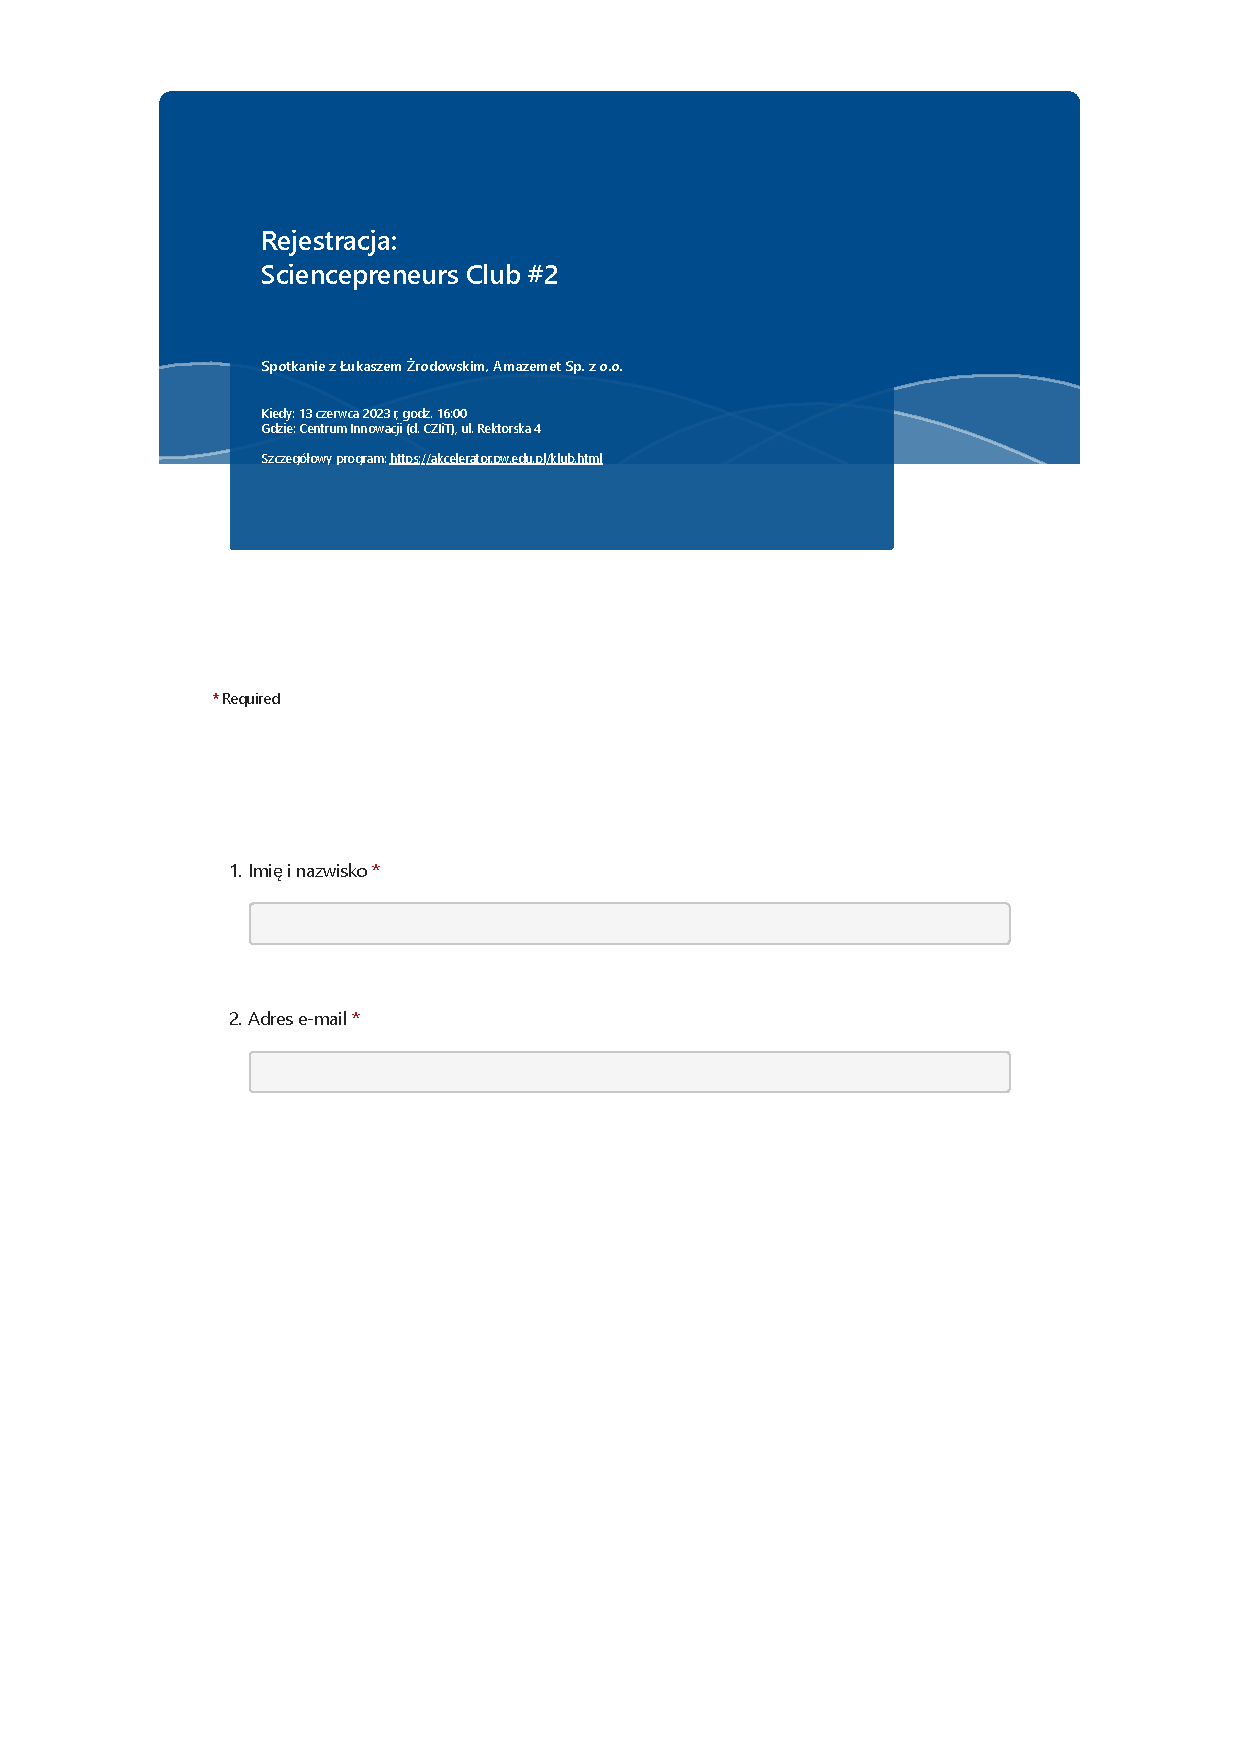
\includepdf[pages=-]{pdf/RejestracjaSciencepreneursClub2.pdf} % Wstawia PDF

% Trzeci załącznik
\chapter{Dodatkowe materiały cyfrowe}
\label{app:materialy}

Pełna konfiguracja systemu oraz instrukcja wideo dostępne są w wersji cyfrowej:  
\begin{itemize}
    \item \textbf{Instrukcja wideo aktualizacji bazy danych} -- plik \texttt{Instrukcja Wideo Aktualizacji \\Baz Danych.mov}
    
    \item \textbf{Baza danych Microsoft Excel} -- plik \texttt{SC BAZA.xlsx}
    
     \item \textbf{Pliki konfiguracji automatyzacji} -- plik \texttt{AktualizacjarejestracjiSC3(froms)dobazy\\(excel).zip}
\end{itemize}

Wszystkie wymienione materiały znajdują się na dołączonym nośniku USB.

\end{document}